\documentclass[portuguese,oneside]{pucrs-ppgcc}

\usepackage{graphicx}
\usepackage{multirow}

% \usepackage{booktabs}
% \usepackage{colortbl}

% \usepackage{afterpage}

\usepackage[breaklinks=true]{hyperref}
\usepackage{breakcites}
\usepackage{spverbatim}
\usepackage{listings}
\usepackage{algpseudocode}

% \usepackage{easy-todo}

% \usepackage{pdflscape}
\usepackage{rotating}

\usepackage{minted}
\usepackage{preview}
\usepackage{subcaption}

\usepackage[capitalize]{cleveref}
\crefname{section}{Section}{Sections}
\Crefname{section}{Sec.}{Secs.}
\crefname{table}{Table}{Tables}
\Crefname{table}{Tab.}{Tabs.}
\crefname{figure}{Figure}{Figures}
\Crefname{figure}{Fig.}{Figs.}
% \crefname{chapter}{Chapter}{Chapters}
% \Crefname{figure}{Fig.}{Figs.}

\hbadness=10000
\vbadness=12000

\lstdefinelanguage{json}{
    basicstyle=\normalfont\ttfamily,
    numbers=left,
    numberstyle=\scriptsize,
    stepnumber=1,
    numbersep=8pt,
    showstringspaces=false,
    breaklines=true,
    frame=lines,
    backgroundcolor=\color{background}
}
%% Create a pair of images on the same row
\newcounter{imagePair}[figure]

\newcommand{\imagePair}[3][0.2]{
    \refstepcounter{imagePair}
    {\small \textbf{\alph{imagePair}.}}\hfill
    \begin{tabular}{@{}c@{}}
        \includegraphics[width=#1\textwidth]{#2}\\
        % {\small \textbf{a.} }
    \end{tabular}
    \hfill
    \begin{tabular}{@{}c@{}}
        \includegraphics[width=#1\textwidth]{#3}\\
        % {\small \textbf{a.} }
    \end{tabular}
    \hfill
}
%%

%% For Changing table lines' width
\newcommand{\thinline}[0]{\specialrule{.05em}{0em}{0em}}

\newcommand{\thickerTableLines}[0]{\setlength{\arrayrulewidth}{.1em}}
\newcommand{\defaultTableLines}[0]{\setlength{\arrayrulewidth}{.05em}}
%%

%% For Table Spacing
\newcommand{\stretchTableCells}[0]{\renewcommand{\arraystretch}{1.5}}
\newcommand{\defaultTableCells}[0]{\renewcommand{\arraystretch}{1}}
%%

%% For Cell Highlighting
\newcommand{\hlCell}[0]{\cellcolor{blue!25}}
%%

%% Create a Blank Page
\newcommand{\blankpage}[0]{\afterpage{\null\newpage}}
%


%% Mention a Dataset ID
\newcommand{\citData}[1]{%
    \hyperref[tab:datasets]{[D0#1]}%
}
%

\author{Gabriel Vaz de Souza}

\title{LODUS-Health: Uma ferramenta para simulação do fluxo de pacientes nos leitos dos hospitais de Porto Alegre.}
      {LODUS-Health: A tool for simulating the flow of patients in hospital beds in Porto Alegre.}

% \tipotrabalho{\pep}         % Plano de estudo e pesquisa (Research plan)
\tipotrabalho{\dissertacao} % Dissertação (Master Thesis)

\versaovolume{\banca}         % Avaliação Banca
% \versaovolume{\final}  % Volume Final para Homologação e Publicação

\grau{\mestre}

\generoori{\orientadora}
\orientador{Soraia Raupp Musse}

% \fichacatalografica{src/ficha_catalografica.png}

% \dataaprovacao{00}{March}{2024}
% \avaliadorum{Prof.1}{PPGCC/PUCRS}
% \avaliadordois{Prof.2}{PPGC/UFRGS}

\begin{document}

\dedicatoria{
Dedico este trabalho à minha família: meus pais, Nelso e Maria de Fátima; meus irmãos, Samuel e Daniel; e minha esposa, Emely. Agradeço pelo amor, apoio e incentivo ao longo desses anos de estudo. Vocês foram minha base, fonte de força e inspiração nessa jornada.

Dedico este trabalho também aos meus orientadores, Prof\textsuperscript{a}. Soraia R. Musse e Prof. Rafael H. Bordini, pela orientação, paciência e crença na minha capacidade ao longo dessa jornada. Suas contribuições foram fundamentais para o desenvolvimento deste estudo e me ajudaram a compreender a importância do que é ser um pesquisador

Dedico aos meus colegas Davide, Gabriel, Marina e Nathalia. Vocês foram essenciais para o desenvolvimento desse estudo; suas dicas, conhecimentos e empenho em me ajudar fizeram com que esse estudo fosse possível.

Por fim, dedico aos meus amigos que compartilharam comigo momentos de alegria e tristeza durante essa jornada.
}

\begin{agradecimentos}
O presente trabalho foi realizado com apoio da Coordenação de Aperfeiçoamento de Pessoal de Nível Superior – Brasil (CAPES) – Código de Financiamento 001.

Esta dissertação foi apoiada pelo Ministério da Ciência, Tecnologia e Inovações, com recursos da Lei no 8.248, de 23 de outubro de 1991, no âmbito do PPI-SOFTEX, coordenado pela Softex e publicado Residência em TIC 02 - Aditivo, DOU 01245.012095/2020-56.
\end{agradecimentos}

\begin{resumo}{Gerenciamento Hospitalar, Ocupação de Leitos Hospitalares, Simulação Urbana, Geração de Dados, Visualização de Dados}
% Contextualização
A área da saúde no Brasil enfrenta diversos desafios decorrentes da escassez de recursos nos hospitais do país~\cite{ORCAMENTOSAUDEBR}. Explorar técnicas que ajudem a mitigar o uso inadequado de recursos e prever cenários de alta demanda no futuro pode ser de grande auxílio para os gestores municipais na alocação eficiente desses recursos.
% Objetivos
Este trabalho visa apresentar o desenvolvimento do LODUS-Health, uma ferramenta que simula o fluxo de pacientes nos leitos dos hospitais de Porto Alegre, possibilitando a configuração dos parâmetros do modelo de simulação pela interação com uma interface gráfica, além de permitir a visualização dos resultados e a geração de textos médicos de evolução de pacientes internados.
% Metodologia
Para isso, criou-se um conjunto de dados a partir das informações do CNES disponibilizadas pelo DATASUS e coordenadas geográficas obtidas no Google Maps. Além disso, foi desenvolvida uma interface gráfica com ferramentas de desenvolvimento web, como o Flask. Utilizou-se o \textit{framework} LODUS como ferramenta central para o deslocamento dos pacientes em um ambiente de simulação virtual. Por fim, foi utilizada a API da OpenAI para geração dos textos médicos.
% Resultados
Os resultados obtidos demonstram que o modelo se comporta conforme o esperado em diferentes configurações de simulação, e a geração de dados mostra-se coerente com a tarefa delimitada.
% Conclusões
Conclui-se que a ferramenta pode ser utilizada para a prevenção da escassez de recursos e gestão hospitalar. No entanto, ressalta-se a importância da utilização um profissional da área para garantir a eficácia dos resultados.
\end{resumo}

\begin{abstract}{Hospital Management, Hospital Bed Occupancy, Urban Simulation, Data Generation, Data Visualization}
The healthcare sector in Brazil faces several challenges due to the scarcity of resources in the country's hospitals~\cite{ORCAMENTOSAUDEBR}. Exploring techniques that help mitigate the inappropriate use of resources and forecast scenarios of high demand in the future can greatly assist municipal managers in efficiently allocating these resources. This work aims to present the development of LODUS-Health, a tool that simulates the flow of patients in the beds of hospitals in Porto Alegre, allowing for the configuration of simulation model parameters through interaction with a graphical interface, as well as enabling the visualization of results and the generation of medical texts documenting the evolution of hospitalized patients. To achieve this, a dataset was created from information provided by CNES available through DATASUS and geographical coordinates obtained from Google Maps. Additionally, a graphical interface was developed using web development tools such as Flask. The LODUS framework was employed as the central tool for patient displacement in a virtual simulation environment. Finally, the OpenAI API was used for the generation of medical texts. The results obtained demonstrate that the model behaves as expected under different simulation configurations, and the data generation is consistent with the defined task. It is concluded that the tool can be used for preventing resource scarcity and hospital management. However, it is emphasized the importance of involving a professional in the field to ensure the effectiveness of the results.
\end{abstract}

\tableofcontents

\chapter{Introdução} \label{cpt:intro}
O desenvolvimento e a pesquisa na área da saúde são temas que causam grandes impactos de forma direta na vida dos cidadãos. 
%GA: adicionar alguma ref sobre eficacia de vacinas abaixo (GV: corrigido)
Um exemplo recente foi a pandemia causada pelo contágio da COVID-19, na qual o desenvolvimento de vacinas pelos laboratórios de pesquisa minimizou a taxa de contágio do vírus, ajudou na prevenção de morbidade e mortalidade e possibilitou o retorno ao convívio social após meses de restrições~\cite{VACINAS}.

Fazer pesquisa na área da saúde não se resume a idealizar soluções, como vacinas. %apenas a nível mundial. 
%SO: Achei estranha a frase acima... parece que queremos fazer algo para além do planeta???? dei uma mexida (GV: corrigido)
Outros contextos de pesquisa também contribuem para o desenvolvimento dessa área. A pesquisa sobre melhorias na gestão de recursos públicos de saúde, por exemplo, também é uma forma de contribuir para o avanço dessa área e tem um impacto importante na população local. Desenvolver uma solução que auxilie as equipes de gestão de municípios a encontrar formas de reduzir os custos na distribuição de recursos nos hospitais da cidade pode resultar em um maior fluxo de atendimentos e até mesmo na destinação de verbas para outras áreas, como segurança e educação, por exemplo, ou ainda ajudar na prevenção da escassez de recursos~\cite{ganesh2023fair}.
%GA: refs acima? (GV: revisar)

O investimento em saúde no Brasil não tem acompanhado as demandas da população e apresentou um cenário de estagnação orçamentária na última década, crescendo apenas 2,5\%~\cite{ORCAMENTOSAUDEBR}. Em Porto Alegre, o orçamento disponibilizado para a saúde em 2024 foi de R\$ 342.149.858,00, valor que inviabiliza o atendimento mínimo das necessidades em saúde do município~\cite{ORCAMENTO}. Considerando um orçamento insuficiente e a tendência de aumento de problemas como precarização e sobrecarga, é necessária a existência de abordagens capazes de contribuir para redução de custos na área da saúde, e o uso da tecnologia pode ser um grande aliado na tentativa de diminuir essas dificuldades. 
%GA: adiciona o sobrenome dos autores quando for falar dos trabalhos deles desta forma. Ex: "Os trabalhos de ABC [14] e DED et al. [4]". Aqui também acho que caberia uma explicação do que são esses trabalhos. 1-2 frases para cada um.  (GV: corrigido)
Os trabalhos de Silva, G. F.~\cite{9239083} e El-Bouri, R. et al.~\cite{9103941} apresentam alguns exemplos de abordagens tecnológicas possíveis de serem utilizadas de modo a contribuir para o desenvolvimento da área da saúde. O primeiro utiliza a abordagem de simulação urbana virtual para fornecer \textit{insights} precisos sobre a dinâmica populacional e oferecer informações cruciais para a tomada de decisões dos gestores urbanos. Já o segundo trabalho visa facilitar a preparação dos espaços de leitos hospitalares através do treinamento de um modelo de aprendizado profundo.

Observando que o orçamento para investimentos em saúde em Porto Alegre é limitado e insuficiente, espera-se que as soluções propostas não tenham um custo elevado para sua implantação. Com isso, simular ambientes urbanos virtuais pode ser uma alternativa de baixo custo a ser explorada na tentativa de redução de custos em saúde.

Ao trabalhar com a simulação de ambientes urbanos virtuais, podemos estudar o comportamento de cenários em diversas situações. A superlotação de estádios de futebol, a transmissão de uma doença contagiosa e o trânsito de pessoas pelos bairros da cidade são alguns exemplos de aplicações. Os resultados dessas simulações podem ser objetos de estudo para prevenir eventos prejudiciais à população, realizar ações de marketing e até mesmo entender o comportamento de eventos ocorridos no passado. São diversas as possibilidades de aplicações. Na área da saúde, simular grupos de pessoas em cidades com muitos habitantes, agregar dados da vida para um ambiente virtual e gerar dados para estudos são alguns dos desafios associados a essa área. Uma aplicação da simulação de um ambiente urbano virtual nesse contexto pode ser empregado para estimar o fluxo de pacientes nos leitos de um ou mais hospitais nas cidades durante um período parametrizado. Essa dissertação visa a proposta de desenvolvimento do LODUS-Health, um simulador que trata de alguns temas da saúde em um ambiente de simulação urbana virtual.

%SO: Aqui falta dizer o desafio da área... p.ex. desafio de simular pessoa por pessoa em cidades com miutos habitantes, necessidade de agregar dados da vida real... e etc... No final dizer que essa dissertação visa desenvolver um simulador que permita tartar de alguns temas da saúde dentro da simulação urbana. (GV: corrigido)

\section{Objetivo}
%GA: para framework e outras palavras estrangeiras, usar itálico (GV: corrigido)
O objetivo deste trabalho é apresentar a pesquisa e desenvolvimento do LODUS-Health, uma ferramenta de simulação do fluxo de ocupação dos leitos hospitalares da cidade de Porto Alegre, 
%SO: Vaz: tu achas que tu tu fizeste um simulador de fluxod e ocupação de leitos, ou seria mais adequado dizer que tu simulas fluxos de pessoas na cidade que se direcionam a ociupar hospitais? ou algo assim (GV: revisar)
visando aprimorar a gestão hospitalar pública em diversos cenários, como na destinação de recursos. Espera-se que a ferramenta seja capaz de prover aos usuários a capacidade de realizar simulações de um ambiente configurado com dados reais de quantidade de leitos hospitalares e permita que usuários especialistas na área da saúde ou gestores urbanos ou hospitalares possam observar o comportamento dos leitos hospitalares em um contexto customizado. Para isso, é desenvolvida uma abordagem de simulação com configurações parametrizáveis utilizando o \textit{framework} de simulação urbana virtual LODUS~\cite{9239083}, geração de textos médicos de evolução de pacientes com a OpenAI API\footnote{\url{https://openai.com/blog/openai-api}} e uma interface gráfica com ferramentas de desenvolvimento web. Conforme será descrito nos resultados, o modelo proposto neste projeto permite a simulação de cenários de ocupação de leitos em diferentes especialidades dentro dos hospitais de Porto Alegre. %GA: ref e footnote para o LODUS e para a API da OpenAI (GV: revisar)

%SO: para ter uma section só para objetivos ela deve incluir objetivos específicos. Exemplos: integrar com dados reais da cidade, como doenças CIDI e dados de hopitais, prover ferramenta ao usuários final que permita blabla.... (GV: corrigido)


%SO: Ao final, uma frase, p.ex.: " Conforme será descrito nos resutlados, o modelo proposto neste projeto permite o desenvolvimento de cenários para simulação urbana e de encaminhamento de doentes aos hospitais. (GV: revisar)

\section{Organização do Trabalho}
Esta pesquisa está organizada nos seguintes capítulos: O Capítulo~\ref{cpt:contexto} contextualiza sobre as principais tecnologias utilizadas no desenvolvimento do modelo de simulação, são descritos o \textit{framework} LODUS e a OpenAI API nas seções \ref{sec:back_lodus} e \ref{sec:chat}. No Capítulo~\ref{cpt:lit}, é apresentada a metodologia utilizada na seleção dos trabalhos relacionados, descrevendo a fonte de busca (Seção~\ref{sec:fontes_busca}), os critérios de inclusão e exclusão (Seção~\ref{sec:criterios}), o processo de seleção de materiais (Seção~\ref{sec:processo_selecao}), os trabalhos relacionados (Seção~\ref{sec:trabalhos_selecao}) e uma breve discussão sobre eles é feita na Seção~\ref{sec:trabalhos_discussao}. O Capítulo~\ref{cpt:met_prop} discorre sobre a metodologia aplicada no desenvolvimento da pesquisa, passando pelas etapas de criação do conjunto de dados utilizado, incluindo a coleta de dados (Seção~\ref{sec:sites}), a estruturação do conjunto de dados e uma análise sobre eles (Seção~\ref{sec:montagem_conjunto}). Também é apresentada as etapas de desenvolvimento da interface gráfica (Seção~\ref{sec:interface_config}), do \textit{plugin} de simulação (Seção~\ref{sec:plugin_lodus}), a visualização dos resultados do modelo de simulação (Seção~\ref{sec:visualizacao_resultados}) e geração de texto médico individualizado (Seção~\ref{sec:geracao_texto}). O Capítulo~\ref{cpt:result} apresenta os resultados da simulação em quatro diferentes contextos. Por fim, os Capítulos~\ref{cpt:discus} e~\ref{cpt:conclus} apresentam uma discussão sobre o trabalho e a conclusão, respectivamente.

%SO: de maneira geral, a section precisa de mais refs (GV: corrigido)
\chapter{Fundamentação Teórica} \label{cpt:contexto}
Este capítulo descreve duas técnicas importantes que são relevantes para o desenvolvimento desta pesquisa. O \textit{framework} LODUS e a OpenAI API são os conteúdos abordados nas seções a seguir.

\section{\label{sec:back_lodus}LODUS}
LODUS é um \textit{framework} que permite simular ambientes urbanos virtuais em vários níveis de detalhes, tendo como objetivo principal prover informações para colaborar com os desafios de planejamento e manutenção de cidades~\cite{9239083}. O LODUS é um modelo multinível capaz de ser configurado de duas formas: i) reproduzindo cenários do mundo real ou ii) simulando dinâmicas urbanas antes de acontecerem na vida real. Em ambos os casos, é importante que o ambiente e a população possam ser coerentemente simulados.

O \textit{framework} permite a representação de um ambiente com diferentes níveis de abstração. Em cada nível, uma representação mais detalhada do ambiente pode ser definida, e a cada inclusão de um nível mais profundo, informações mais detalhadas podem ser computadas. Esses detalhes armazenam dados diversos, como distribuição populacional, sistema viário, geometria dos edifícios ou até mesmo configurações internas dos edifícios.

Dentro do LODUS, uma cidade pode ser definida por um Grafo de Região, esse grafo representa conexões entre regiões próximas. A Figura~\ref{fig:lodus}(a) abaixo demonstra a representação da cidade de Porto Alegre por um Grafo de Região, ao lado, a Figura~\ref{fig:lodus}(b) mostra a delimitação territorial da cidade no mundo real. Cada região do grafo está relacionada a um bairro dentro da cidade que possui seus pontos de interesse, por exemplo, casas, hospitais, postos de combustível, escolas e etc. Um ponto de interesse no ambiente tem suas características próprias e pode ser configurado no nível de detalhes desejado, por exemplo, pode se atribuir a um ponto de interesse a quantidade de pessoas nele e agrupá-las por idade, gênero, ocupação e etc. 

O \textit{framework} possibilita que dentro da simulação, pontos de interesse recebam populações de outros pontos de interesse com características especificas ou não, por exemplo, hospitais na região recebem populações que estão em casas, escolas, estádios de futebol e etc. Essas decisões de fluxo de população são parametrizáveis nas configurações.

\begin{figure}
    \centering
    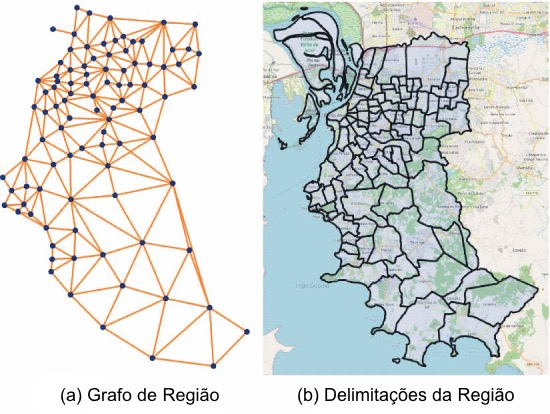
\includegraphics[width=12cm]{Capitulos/images/graph-region.jpeg}
    \caption{Grafo de Região do LODUS~\cite{9239083}.%GA: ref para a minha minha dissertação. Ajustar o crop da parte de baixo da imagem e esta com um pouco da legenda original.
    %GA: explicar as etapas na caption desta figura, mesmo que fique um pouco redundante com o texto (não copiar)
    %GA: As subfigures (que não são subfiguras no latex) estão com captions em inglês, tentar manter coerencia com o texto ou explicar o que é cada uma.
    }
    \label{fig:lodus}
\end{figure}

% \begin{figure}
%     \centering
%     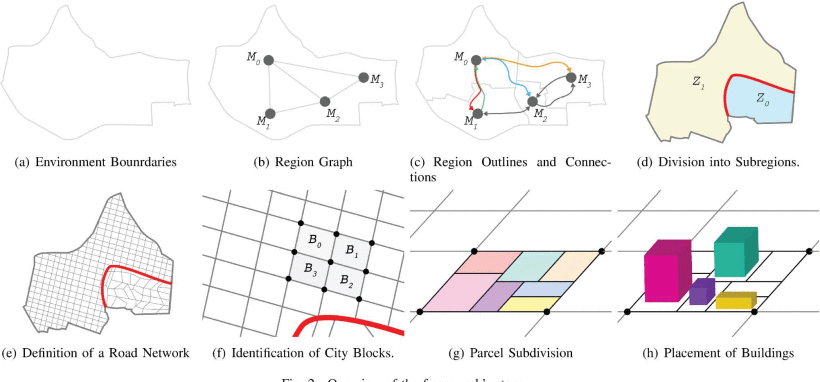
\includegraphics[width=\textwidth]{Capitulos/images/lodus-overview.png}
%     \caption{Visão geral dos estágios do framework.%GA: ref para a minha minha dissertação. Ajustar o crop da parte de baixo da imagem e esta com um pouco da legenda original.
%     %GA: explicar as etapas na caption desta figura, mesmo que fique um pouco redundante com o texto (não copiar)
%     %GA: As subfigures (que não são subfiguras no latex) estão com captions em inglês, tentar manter coerencia com o texto ou explicar o que é cada uma.
%     }
%     \label{fig:lodus}
% \end{figure}

% Na Figura~\ref{fig:lodus}(a), são ilustrados os Limites do Ambiente, representados em um plano 2D. Podemos definir o ambiente como um conjunto de Regiões, onde cada Região é um ponto 2D colocado dentro dos limites do ambiente. Uma Região pode representar diferentes áreas de acordo com o nível de abstração desejado, como: grupos de blocos da cidade dentro de um bairro; bairros dentro de uma única cidade; cidades dentro de uma área metropolitana; condados dentro de um estado; e estados dentro de um país.

% O Grafo de Região, conforme mostrado em Figura~\ref{fig:lodus}(b), pode ser especificado como um grafo não direcionado G=(P,E), onde P é um conjunto de nós (Regiões) e E contém um conjunto de arestas conectando os nós. Como um grafo planar pode ser aninhado dentro de um nó de outro grafo, é possível definir diferentes níveis de abstração para o Grafo de Região.

% Para permitir a criação de uma rede viária e a representação geométrica dos edifícios, cada região M também é representada por um Contorno (Figura~\ref{fig:lodus}(c)). O contorno de uma região é um polígono descrito por um conjunto de vértices que representam sua geometria.

% A seguir, uma conexão representa uma rota que permite o movimento de M\textsubscript{a} para M\textsubscript{b} por meio de uma lista ordenada de pontos 2D no espaço, onde cada ponto está dentro da geometria de O\textsubscript{a} $\cup$ O\textsubscript{b}. As conexões entre regiões são direcionais, mas podem ser usadas no sentido contrário se desejado pelo usuário e permitido pelas restrições do ambiente (ou seja, representação de rua de duas vias). Segmentos de uma conexão também podem ser compartilhados entre diferentes regiões para permitir movimento em rotas similares.

% Para representar o layout urbano em um nível mais baixo de abstração, é necessário estabelecer uma Rede Viária (Figura~\ref{fig:lodus}(e)) dentro de cada Região do ambiente. Uma Estrada (Q) é definida por uma lista de pontos 2D no espaço, onde cada par de pontos ([Q[i], Q[i+1]]) representa um segmento de estrada. Um conjunto de pontos em uma estrada pode ser compartilhado com um Contorno, permitindo que a estrada represente os limites de uma Região. Para preservar as propriedades de um grafo planar herdadas pelo Grafo de Região, os segmentos de estrada não podem se cruzar. Em casos de interseções, um novo ponto é colocado no ambiente e a lista em cada estrada é ajustada para compreender o novo segmento. Apesar de compartilharem a mesma estrutura, o framework distingue as estradas em "primárias" (ou seja, estradas arteriais, avenidas principais ou rodovias) e "secundárias" (ou seja, ruas locais), devido aos seus propósitos em cada etapa.

% As estradas primárias atravessam grandes partes do contorno de uma Região e são responsáveis por dividir o contorno em Subregiões (Figura\ref{fig:lodus}(d)), representando uma segmentação de um Contorno. As estradas secundárias fornecem acesso local para diferentes áreas dentro de uma Subregião e podem ter um comprimento menor. Os pontos extremos de uma estrada primária devem pertencer ao contorno da Região ou a outra estrada primária. Essa restrição é aplicada para manter as propriedades do grafo planar. Um conjunto de parâmetros é definido para descrever as estradas em maior detalhe e permitir a integração com outras aplicações, por exemplo, simulação de tráfego.

% Após a formação da rede de estradas secundárias, é possível obter um conjunto de quadras (Figura\ref{fig:lodus}(f)) dentro de cada Subregião. Uma quadra também é representada por um conjunto de pontos 2D formando um polígono. Cada ponto em uma quadra pertence a um segmento de estrada secundária ou ao contorno da Subregião. As quadras compreendem um conjunto de lotes (Figura\ref{fig:lodus}(g)), que são usados como base para a geração de edifícios e casas (Figura\ref{fig:lodus}(h)). As quadras dentro da mesma Subregião podem compartilhar um conjunto padrão de propriedades para dar a elas uma aparência semelhante. Como uma quadra pode conter vários lotes, um algoritmo de subdivisão é aplicado às quadras desejadas com uma área grande o suficiente.



%GA: no caso deste trabalho, acho que a movimentação entre regiões e bairros é mais relevantes de comentar, pq tu não chega a utilizar as ruas em si ou uma API de rotas
Nesta pesquisa, o LODUS é utilizado como ferramenta central no desenvolvimento do modelo de simulação. Um ambiente simulando os bairros, ruas e estradas da cidade de Porto Alegre é empregado, e um \textit{plugin} customizado é adicionado para possibilitar o contexto de fluxo de ocupação hospitalar dentro da simulação.

\section{\label{sec:chat}OpenAI API}
A API da OpenAI oferece acesso a poderosas ferramentas de inteligência artificial desenvolvidas pela OpenAI. Ela permite que os desenvolvedores integrem facilmente modelos de linguagem avançados, como o GPT-3 (\textit{Generative Pre-trained Transformer})~\cite{brown2020language}, em suas próprias aplicações. %GA: tem alguma ref para o GPT-3? acho que deve ter algum paper publicado deles (GV: corrigido)
Atualmente, a API fornece uma interface ``\textit{text in, text out}'' de propósito geral, possibilitando a integração da API em produtos existentes, novas implementações ou ajudando a OpenAI a explorar os limites dessa tecnologia~\cite{OPENAI}.

Dado qualquer \textit{prompt} de texto, a API retornará um texto de resposta, tentando corresponder ao padrão fornecido. A API pode ser programada a partir de alguns exemplos nos quais o usuário gostaria que o resultado fosse semelhante, e a qualidade dos resultados geralmente varia dependendo da complexidade da tarefa. Além disso, a API permite aprimorar o desempenho em tarefas específicas com o treinamento de conjuntos de dados de exemplos fornecidos ou por meio de \textit{feedback} humano de usuários ou rotuladores. Ela pode ser aplicada em diversos contextos para enriquecer a interação humano-computador. A seguir está listada uma visão simplificada do funcionamento da API.

\begin{itemize}
    \item Requisição e Autenticação: Um usuário envia uma solicitação para a API da OpenAI, geralmente contendo um \textit{prompt} de entrada, que é o texto inicial para o qual deseja uma resposta. A autenticação é realizada usando credenciais de API, garantindo que apenas usuários autorizados tenham acesso.

    \item Processamento: A API recebe a solicitação e a processa internamente. Isso envolve analisar o \textit{prompt} de entrada, entender o contexto e determinar qual modelo de linguagem e quais parâmetros usar para gerar uma resposta adequada.

    \item Modelo de Linguagem: A API utiliza modelos de linguagem avançados, como o GPT, para gerar respostas. Esses modelos são treinados em grandes conjuntos de dados para entender a estrutura da linguagem natural e gerar texto coerente e relevante.

    \item Geração de Resposta: Com base no \textit{prompt} de entrada, o modelo de linguagem gera uma resposta correspondente. Isso envolve a geração de texto novo, seguindo o contexto fornecido pelo \textit{prompt}, bem como qualquer informação adicional, como configurações específicas do modelo.

    \item Retorno da Resposta: A resposta gerada pelo modelo é então enviada de volta ao usuário como a saída da API. Isso geralmente acontece em tempo real, dependendo da complexidade da solicitação e da carga de trabalho do servidor.

\end{itemize}

Em resumo, a API da OpenAI utiliza modelos de linguagem avançados para compreender e gerar texto em resposta às solicitações dos usuários, oferecendo uma interface simples para a integração de inteligência artificial em uma variedade de aplicativos e cenários. A Figura~\ref{fig:openai-flow} apresenta, de maneira geral, um exemplo do fluxo de comunicação com a API.

\begin{figure}
    \centering
    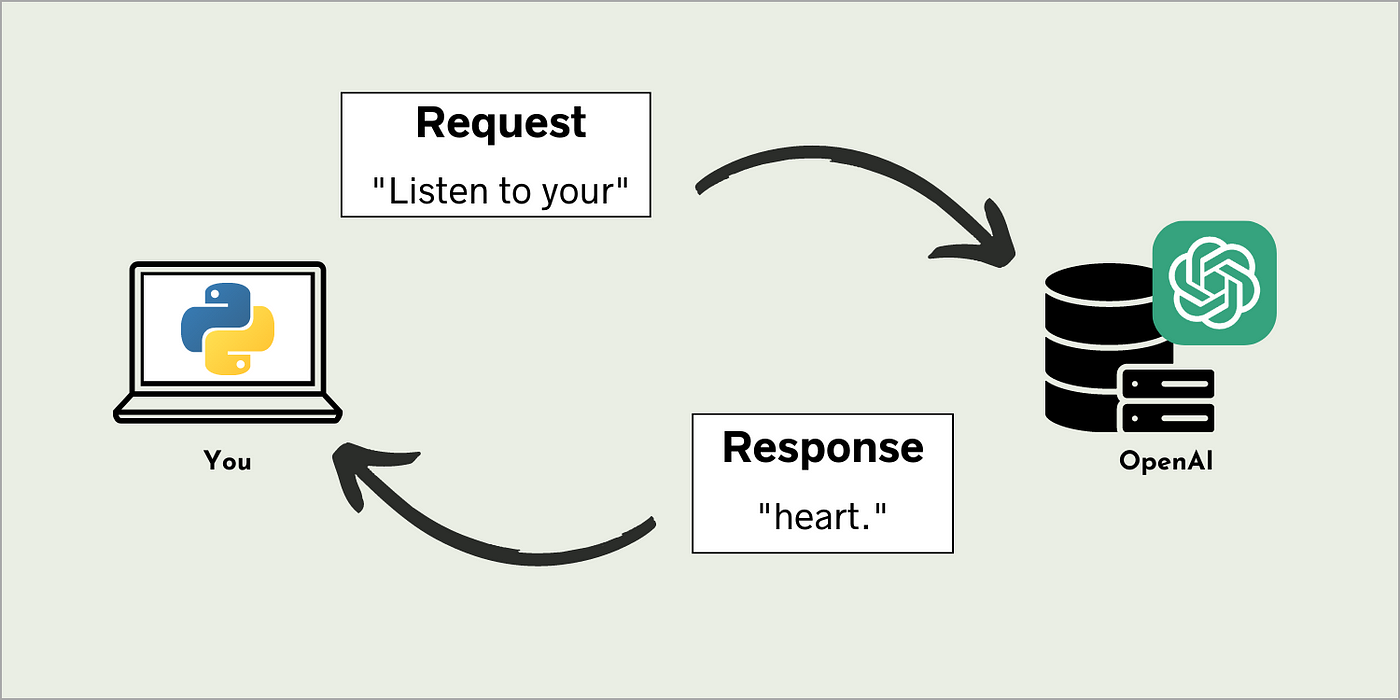
\includegraphics[width=0.75\textwidth]{Capitulos/images/openai-api.png}
    \caption{Fluxo de comunicação da API~\cite{OPENAIIMAGE}.}
    \label{fig:openai-flow}
\end{figure}

No desenvolvimento desta pesquisa, a API é utilizada para a geração de textos de internação hospitalar para uma determinada especialidade de internação selecionada pelo usuário na interface, dependendo dos parâmetros de configuração utilizados na simulação.
\chapter{Trabalhos Relacionados} \label{cpt:lit}
%SO: Vaz: nesta seção, ajuste as frases para que não fique "No trabalho de [1]..." isso é muito deselegante... coloque o nome do autor. (GV: corrigido)
Neste capítulo, discutimos a metodologia empregada no processo de seleção dos trabalhos da literatura, abordando as fontes de busca, os parâmetros utilizados para inclusão e exclusão, os critérios de seleção de materiais, os trabalhos selecionados e uma breve discussão sobre os resultados obtidos.

\section{\label{sec:fontes_busca}Fontes de Busca}
As fontes utilizadas para encontrar trabalhos relacionados a esta pesquisa foram classificadas em, nível 1 (alta credibilidade) e nível 2 (moderada credibilidade). Fontes classificadas como nível 3 (baixa credibilidade) não foram incluídas na busca. Abaixo está a lista das fontes selecionadas, todas classificadas como níveis 1 e 2.

\begin{itemize}
    \item Biblioteca Digital do IEEE (http://ieeexplore.ieee.org/Xplore/) - Nível 1
    \item Biblioteca Digital da ACM (http://portal.acm.org/) - Nível 1
    \item arXiv: (http://https://arxiv.org/) - Nível 2
\end{itemize}

A seguinte \textit{string} de busca foi utilizada para encontrar trabalhos relacionados à área na literatura. Essa \textit{string} de busca foi elaborada considerando termos-chave relevantes no contexto da pesquisa.

\begin{center}
((``\textit{simulating environment}'' OR ``\textit{simulated environment}'' OR ``\textit{crowd simulation}'') AND (\textit{population} OR \textit{hospital} OR ``\textit{hospital bed}'' OR ``\textit{admission}'' OR ``\textit{public}'')) OR (\textit{hospital} AND (\textit{bed} OR \textit{admission}))
\end{center}

\section{\label{sec:criterios}Critérios de Inclusão e Exclusão}
Na Tabela~\ref{table:1} a seguir, são apresentados os critérios de inclusão e os critérios de exclusão utilizados com o objetivo de assegurar a relevância dos estudos na seleção de trabalhos relacionados e filtrar os resultados encontrados nas bases de dados apresentados na Seção~\ref{sec:fontes_busca}.

\begin{table}[h!]
\centering
\begin{tabular}{ |m{15em}|m{15em}| } 
 \hline
 Critérios de inclusão & Critérios de exclusão \\ 
 \hline
 Soluções para ocupação de leitos hospitalares. & Publicado antes do ano de 2020.\\[0.5cm]
 Aplicações de simulação de multidão em ambientes públicos.  & Não apresentem soluções tecnológicas.\\[0.5cm]
& Materiais com acesso pago.\\[0.5cm]
 & Escrita em idiomas diferentes de inglês ou português.\\
 \hline
\end{tabular}
\caption{Critérios de inclusão e exclusão.}
\label{table:1}
\end{table}

\section{\label{sec:processo_selecao}Processo de Seleção de Materiais}
Para a seleção dos materiais, realizou-se uma busca nas fontes mencionadas na Seção~\ref{sec:fontes_busca}, utilizando a \textit{string} de busca também fornecida na mesma seção. A pesquisa resultou em 3.205 trabalhos, distribuídos em 1.261 do IEEE, 2.401 da ACM e 145 do arXiv. Após a aplicação dos critérios de inclusão e exclusão, restaram 69 trabalhos, sendo 17 do IEEE, 15 da ACM e 27 do arXiv. Posteriormente, após a leitura dos resumos e avaliação, foram selecionados 8 trabalhos, sendo 4 da IEEE, 2 da ACM e 2 do arXiv. Na Tabela~\ref{table:2} abaixo estão listados os resultados da seleção de materiais.

\begin{itemize}
    \item F1: Número de trabalhos encontradas na busca; 
    \item F2: Número de trabalhos selecionados com base nos critérios de inclusão e exclusão;
    \item F3: Número de trabalhos selecionados.
\end{itemize}

\begin{table}[h!]
\centering
\begin{tabular}{ |c|c|c|c| } 
 \hline
 Fonte & F1 & F2 & F3 \\ 
 \hline
 IEEE & 1.261 & 17 & 4\\ 
 ACM & 2.401 & 15 & 2\\ 
 arXiv & 145 & 37 & 2\\ 
 \hline
\end{tabular}
\caption{Número de trabalhos selecionados por fonte de busca.}
\label{table:2}
\end{table}

\section{\label{sec:trabalhos_selecao}Trabalhos Selecionados}
No trabalho de El-Bouri, R. et al.~\cite{9103941}, os autores apresentam a implementação de um modelo de aprendizado profundo com o objetivo de prever a área de internação de pacientes na emergência de um hospital após a triagem no departamento de emergência (DE). Essa previsão visa facilitar a preparação dos espaços de leitos hospitalares para atender e internar os pacientes de forma oportuna, além de alocar recursos para os departamentos relevantes, especialmente durante períodos de aumento de demanda causados por picos sazonais de infecções. O problema foi abordado pelos autores como uma questão de classificação multiclasse em sete tipos de enfermarias. Foi desenvolvida uma estratégia de treinamento de aprendizado profundo que combina a aprendizagem por meio de currículo e o \textit{Multi-armed bandit} para explorar esse currículo de treinamento pós-inicial. Como resultado, foi previsto com sucesso o local inicial de internação hospitalar, com a área sob a curva ROC (AUC) variando entre 0,60 e 0,78 para as enfermarias individuais e uma precisão máxima geral de 52\%, quando a chance aleatória corresponde a 14\% para esse ambiente de sete classes. A rede proposta foi capaz de interpretar quais recursos impulsionaram as previsões, utilizando um termo de "saliência de rede" adicionado à função de perda da rede. Os autores demonstraram que é possível prever o local de internação hospitalar para pacientes de emergência utilizando informações da triagem no DE, mostrando também que certos testes reveladores indicam qual espaço do hospital um paciente utilizará. Eles esperam que este preditor seja valioso para as instituições de saúde, permitindo o planejamento de recursos e leitos antes da necessidade. Isso, por sua vez, deverá agilizar a prestação de cuidados ao paciente e permitir o fluxo de pacientes para fora do DE, melhorando assim o fluxo de pacientes e a qualidade dos cuidados para os pacientes restantes dentro do DE.

% An Intelligent Scheduling of Non-Critical Patients Admission for Emergency Department
E. Bruballa et al.~\cite{8945359} discutem que o aumento da taxa de envelhecimento da população, juntamente com o aumento da expectativa de vida e da prevalência de doenças crônicas, contribuem para a crescente demanda por cuidados médicos. Eles destacam o problema da sobrecarga nos departamentos de emergência (DE), atribuindo-o, em parte, à internação de pacientes não urgentes, que representam uma parcela significativa dos casos atendidos nos DEs. Como solução proposta, os autores apresentam o uso de um Modelo Baseado em Agentes (ABM) para agendar o acesso de pacientes não críticos aos DEs. Supõe-se que realocar esses pacientes não críticos dentro do padrão de entrada esperado, inicialmente fornecido pelos registros históricos, poderá reduzir o tempo de espera de todos os pacientes, resultando em uma melhoria na qualidade do serviço e evitando longos tempos de espera. Esta pesquisa oferece \textit{insights} relevantes para os gestores do Serviço de Urgência, auxiliando-os a tomar decisões para melhorar a qualidade do serviço, prevendo a crescente demanda que se espera em um futuro próximo. Concluiu-se que a implementação do modelo no simulador de DE e os resultados da análise dos dados da simulação validam a eficácia do modelo, melhorando globalmente o tempo de espera dos pacientes no sistema e, consequentemente, a qualidade dos cuidados de saúde. É importante mencionar que a eficiência da implementação do modelo em um serviço real de DE dependerá da capacidade do sistema de agendamento proposto em gerenciar a entrada real de pacientes, o que está sujeito às decisões dos pacientes ou usuários dos serviços de saúde.

% Bed Allocation Optimization Based on Survival Analysis, Treatment Trajectory and Costs Estimations
O trabalho de Karbouband, K. et al.~\cite{10078258} discute a importância das unidades de terapia intensiva no fluxo de pacientes, destacando desafios como alta demanda, capacidade insuficiente e distribuição injusta de recursos. Os autores propõem uma abordagem inovadora para resolver problemas de alocação de leitos de pacientes, restritos por metas na estimativa da função de sobrevivência, na estimativa de custos e na estimativa da trajetória de tratamento possível para pacientes com doenças cardiovasculares. Para estimativas da função de sobrevivência, foi utilizado o estimador "nave" e Kaplan-Meier, e para estimativas do efeito do tratamento, utilizou-se regressão logística e T-learning. As estimativas dos três componentes são usadas como pesos em um algoritmo genético. Essa técnica permite a consideração de várias restrições, o que, ao contrário de outras técnicas, permite a seleção de soluções dominantes como soluções que satisfazem restrições dominantes. Além disso, foi demonstrado a robustez da abordagem utilizando os algoritmos com múltiplas classes de pacientes, testando múltiplos conjuntos de parâmetros e comparando os resultados com vários estudos de pesquisa semelhantes, mostrando o valor agregado de trabalhar nesse eixo de gestão em hospitais usando a nova abordagem para alocação de leitos.

% Solving the Emergency Care Patient Pathway by a New Integrated Simulation-Optimisation Approach
Em Allihaibi, W. G. et al.~\cite{9481128}, os autores abordam um dos objetivos mais críticos do sistema de saúde, que é maximizar o fluxo de pacientes no atendimento de emergência. A análise do fluxo de emergência do paciente indica que o cronograma de movimentação de um paciente de uma atividade para outra através do departamento de emergência (DE) é fundamental para o tratamento dos pacientes. Quaisquer atividades atrasadas no fluxo de pacientes reduzem o nível de serviço de saúde. Para enfrentar esses desafios, os autores apresentam o desenvolvimento de uma abordagem estocástica de simulação-otimização de DE, considerando variáveis estocásticas, como tempos entre chegadas de pacientes e tempos de tratamento, usando distribuições estatísticas. Este tipo de distribuição depende de dois elementos principais: turnos diurnos e categorias de pacientes. Um algoritmo evolutivo híbrido é integrado à simulação para encontrar uma solução satisfatória para este problema de otimização estocástica em tempo real. Experimentos computacionais mostram que a abordagem proposta pode atender mais pacientes em janelas de tempo específicas ou fornecer a mesma qualidade de serviço com o uso de menos recursos médicos.

% Fair Healthcare Rationing to Maximize Dynamic Utilities
Ganesh, A. et al.~\cite{ganesh2023fair} descrevem um problema relacionado à alocação de recursos de saúde em uma sociedade moderna, especialmente sob condições de recursos logísticos e infraestruturais limitados. Eles propõem um modelo que aborda a alocação de recursos, como vacinas para pessoas ou leitos hospitalares para pacientes, de forma online, considerando a chegada de recursos diariamente, diferentes categorias de agentes, possíveis indisponibilidades de agentes em determinados dias e a utilidade associada a cada alocação, variando ao longo do tempo. O modelo proposto prioriza as diferentes categorias com base na utilidade dos agentes e oferece algoritmos online e offline para calcular alocações que respeitem a elegibilidade dos agentes em diferentes categorias, incentivando-os a não esconder sua elegibilidade. O algoritmo offline oferece uma alocação ótima, enquanto o algoritmo online fornece uma aproximação da alocação ótima em termos de utilidade total. Os algoritmos são eficientes e mantêm a equidade entre as diferentes categorias de agentes. O modelo tem aplicações em áreas como assentamento de refugiados e alocação de vistos. A performance dos algoritmos é avaliada em conjuntos de dados reais e sintéticos, demonstrando que o algoritmo online é rápido e supera a cotação teórica em termos de utilidade total, e confirmando que o modelo baseado em utilidade captura corretamente as prioridades das categorias.

% LODUS: A Multi-Level Framework for Simulating Environment and Population -- A Contagion Experiment on a Pandemic World
Em Silva, G. F. et al.~\cite{9239083}, os autores discorrem sobre a significativa carga de trabalho imposta repentinamente aos gestores urbanos devido à pandemia causada pelo Covid-19, o que os levou a enfrentar o desafio de desenvolver estratégias para conter a propagação da pandemia. Os autores destacam que os ambientes urbanos devem ser dinâmicos e que os gestores precisam tomar decisões rápidas ao lidar com situações de crise. No estudo, é apresentado o LODUS, um \textit{framework} capaz de simular ambientes urbanos por meio de uma abordagem multinível, combinando informações de macro e micro simulação para fornecer \textit{insights} precisos sobre a dinâmica populacional. Além disso, o \textit{framework} LODUS representa uma ferramenta poderosa para conduzir estudos de viabilidade urbana, uma vez que os resultados da simulação têm a capacidade de identificar e prever pontos críticos antes da construção de um ambiente urbano.

% Interactive Simulation of Disease Contagion in Dynamic Crowds
Flor, A. et al.~\cite{10.1145/3487983.3488298}, propõem uma formulação de contágio-imunidade de agente para agente que pode simular a propagação detalhada da COVID-19 dentro de multidões em movimento. Especificamente, os autores desenvolveram um modelo de contágio de doenças baseado em difusão para sistemas discretos que considera o efeito de intervenções de saúde, como distanciamento social, imunidade e vacinação. Integrando sua formulação de contágio-imunidade com as equações governantes de movimento para dinâmica de multidões, eles investigaram a distribuição da doença em multidões com diferentes números de pessoas. Para a mesma simulação de multidão, seu modelo pode simular interativamente a propagação do vírus para diferentes distribuições iniciais de pessoas infectadas. Seus resultados numéricos para o número de pessoas infectadas em multidões densas e não protegidas concordam com o modelo SIS, enquanto seu modelo fornece informações mais ricas sobre a propagação da doença e mostra que a vacinação é a melhor intervenção de saúde para prevenir a infecção.

% Hospital Selection in Emergency Medical Services: A Discrete Event Simulation Approach to Test Different Policies
O trabalho de Tedesco, D. et al.~\cite{10.1145/3587889.3587893} tem como objetivo desenvolver um modelo de simulação para testar e comparar diferentes políticas de seleção de hospitais com o propósito de melhorar a gestão dos sistemas de Serviço Médico de Emergência (EMS, na sigla em inglês). A análise da literatura revelou que a atribuição de pacientes aos departamentos de emergência (EDs) pode ser baseada em diferentes políticas, mesmo que a predominante seja a proximidade (ou seja, minimização da distância entre o local do pedido de emergência e o ED). De fato, estudos atuais são principalmente baseados em ambulâncias, com foco nas fases do EMS relacionadas ao serviço de ambulância, negligenciando assim questões relacionadas ao ED, que são vistas como parte de um processo separado. O objetivo desta pesquisa é mostrar os benefícios de tomar a decisão de seleção de hospital também considerando informações relacionadas à variedade de casos no ED, os tempos esperados de atendimento e a capacidade operacional do ED. Para isso, foi desenvolvido e implementado um modelo de Simulação de Eventos Discretos no AnyLogic para testar diferentes políticas de atribuição. O melhor critério para atribuir pacientes aos EDs foi a minimização do Tempo Até o Provedor (TTP), considerado como o tempo desde o início da jornada da ambulância até o início da avaliação clínica no ED. De fato, esse critério permite reduzir significativamente os tempos de atendimento e situações de superlotação nos EDs. Os resultados desta pesquisa poderiam apoiar os tomadores de decisão na melhoria do desempenho do EMS, introduzindo políticas mais eficazes para o problema de seleção de hospitais.

A Tabela~\ref{table:3} a seguir apresenta os trabalhos selecionados, descrevendo brevemente suas principais características, com o objetivo de facilitar a comparação entre eles.

%%aqui tabela de comparacao
\begin{longtable}{ |c|c|c|p{8.5cm}| } 
% \centering
% \begin{tabular}{ |c|p{10cm}| } 
 \hline
 Trabalho & Ano & Autores & Principais características \\ 
 \hline
 ~\cite{9103941} & 2021 & El-Bouri, R. et al. & Visam facilitar a preparação dos espaços de leitos hospitalares através do treinamento de um modelo de aprendizado profundo que combina aprendizagem por meio de currículo e o \textit{Multi-armed bandit}.\\
 \hline
 ~\cite{8945359} & 2020 & Bruballa, E. et al. & Objetivam agendar o acesso de pacientes não críticos aos DEs, visando reduzir o tempo de espera de todos os pacientes e melhorar a qualidade do serviço, com a implementação de um Modelo Baseado em Agentes (ABM) no simulador de DE.\\
 \hline
 ~\cite{10078258} & 2023 & Karbouband, K. et al. & Descrevem uma abordagem para resolver problemas de alocação de leitos de pacientes nas UTIs, baseada em estimativas da função de sobrevivência, custos e trajetória de tratamento para pacientes com doenças cardiovasculares. Utilizam estimadores para a função de sobrevivência, regressão logística e T-learning para estimativas do efeito do tratamento, incorporando-os como pesos em um algoritmo genético.\\
 \hline
 ~\cite{9481128} & 2021 & Allihaibi, W. G. et al. & Desenvolvem uma abordagem estocástica de simulação-otimização de DE para maximizar o fluxo de pacientes no atendimento de emergência, utilizando distribuições estatísticas para modelar variáveis como tempos entre chegadas de pacientes e tempos de tratamento. Integraram um algoritmo evolutivo híbrido à simulação para encontrar soluções para o problema de otimização em tempo real.\\
 \hline
 ~\cite{ganesh2023fair} & 2023 & Ganesh, A. et al. & Propõem um modelo que aborda a alocação de recursos, como vacinas e leitos hospitalares, de forma online, considerando a chegada diária de recursos. Priorizam diferentes categorias com base na utilidade dos agentes e oferecem algoritmos online e offline para calcular alocações que respeitem a elegibilidade dos agentes.\\
 \hline
 ~\cite{9239083} & 2020 & Silva, G. F. et al. & Apresentam o LODUS, um \textit{framework} capaz de simular ambientes urbanos usando uma abordagem multinível. Ele combina informações de macro e micro simulação para fornecer \textit{insights} precisos sobre a dinâmica populacional e oferecer informações cruciais para a tomada de decisões dos gestores urbanos.\\
 \hline
 ~\cite{10.1145/3487983.3488298} & 2021 & Flor, A. et al. & Desenvolvem um modelo de contágio de doenças baseado em difusão para sistemas discretos, considerando intervenções de saúde, como distanciamento social, imunidade e vacinação. Integraram a formulação de contágio-imunidade com as equações governantes de movimento para a dinâmica de multidões.\\
 \hline
 ~\cite{10.1145/3587889.3587893} & 2023 & Tedesco, D. et al. & Propõem considerar informações relacionadas à variedade de casos no DE, os tempos esperados de atendimento e a capacidade operacional do DE ao tomar a decisão de seleção de hospital. Desenvolvem um modelo de Simulação de Eventos Discretos no AnyLogic para testar diferentes políticas de atribuição de pacientes aos DEs.\\
 \hline
% \end{tabular}
\caption{Características dos trabalhos selecionados.}
\label{table:3}
\end{longtable}

\section{\label{sec:trabalhos_discussao}Discussão}
Após revisar os estudos selecionados, é possível observar uma diversidade de abordagens e soluções propostas para lidar com desafios relacionados ao atendimento hospitalar e à gestão de sistemas de saúde. Nesta seção, discute-se os principais resultados e implicações desses estudos, bem como as contribuições significativas para o desenvolvimento e a pesquisa nessa área.

Vários estudos exploram o uso da inteligencia artificial para melhorar a eficiência e a qualidade dos cuidados de saúde. No trabalho de~\cite{9103941}, por exemplo, mostrou como modelos de aprendizado profundo podem ser utilizados para prever a área de internação de pacientes na emergência de um hospital, facilitando o planejamento de recursos e alocando os pacientes de forma mais eficaz. Essa abordagem promete agilizar o fluxo de pacientes, melhorando assim a qualidade dos cuidados e reduzindo o congestionamento nos departamentos de emergência.

Outros trabalhos se concentraram na modelagem e simulação de sistemas de saúde para otimizar o uso de recursos e melhorar a gestão de filas e tempos de espera. O trabalho~\cite{9481128}, por exemplo, desenvolveu uma abordagem estocástica de simulação-otimização para analisar o fluxo de pacientes em departamentos de emergência, demonstrando como essa técnica pode aumentar a capacidade de atendimento e melhorar a eficiência do sistema de saúde.

Alguns estudos abordaram desafios específicos enfrentados pelos gestores hospitalares e propuseram soluções inovadoras para lidar com esses problemas. O trabalho~\cite{10.1145/3587889.3587893}, por exemplo, examinou diferentes políticas de seleção de hospitais para pacientes de emergência, demonstrando como a minimização do tempo até o provedor pode reduzir os tempos de espera e melhorar o acesso aos cuidados de saúde.

O trabalho~\cite{9239083} destacou os desafios enfrentados pelos gestores urbanos durante a pandemia COVID-19 e apresentou o LODUS, um \textit{framework} para simular ambientes urbanos e fornecer \textit{insights} sobre a dinâmica populacional. Essa abordagem pode ser útil para prever e mitigar futuras crises de saúde pública, fornecendo informações valiosas para os planejadores urbanos e autoridades de saúde.

De maneira geral, os estudos revisados destacam a importância de abordagens inovadoras e o uso de tecnologias na gestão hospitalar e no planejamento de sistemas de saúde. Essas soluções têm o potencial de melhorar significativamente a qualidade dos cuidados de saúde, otimizar o uso de recursos e garantir um acesso mais equitativo aos serviços de saúde. Esse pesquisa visa apresentar uma outra abordagem a ser utilizada como tecnologia na gestão hospitalar, utilizando o \textit{framework} LODUS de~\cite{9239083} no contexto de fluxo de internações, possibilitando que outros trabalhos possam validar seus resultados em um ambiente simulado.
\chapter{Modelo Proposto} \label{cpt:met_prop}
Este capítulo discorre sobre as etapas do desenvolvimento do LODUS-Health, uma ferramenta de simulação de fluxo de ocupação de leitos nos hospitais de Porto Alegre visando aprimorar a gestão hospitalar e urbana. A Figura~\ref{fig:metod} apresenta o fluxo de desenvolvimento da pesquisa, bem como o processo de execução do modelo final. Nas seções a seguir, são abordadas cada uma das etapas desse fluxo.

\begin{figure}
    \centering
    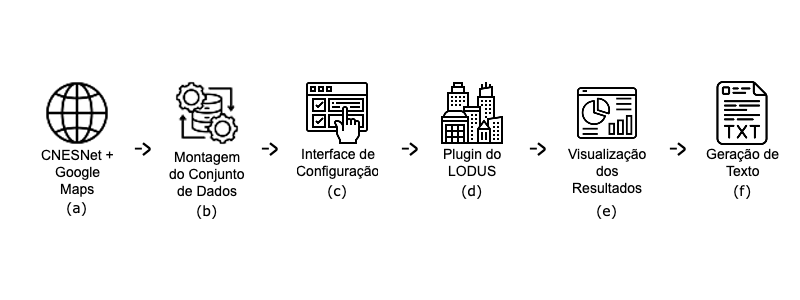
\includegraphics[width=\textwidth]{Capitulos/images/metodologia.png}
    \caption{Visão geral dos estágios de desenvolvimento do modelo.}
    \label{fig:metod}
\end{figure}

\section{CNESNet e Google Maps} \label{sec:sites}
A primeira etapa do fluxo de desenvolvimento representada pela Figura~\ref{fig:metod}(a) é a etapa de busca por dados de informações hospitalares em endereços eletrônicos para a montagem do conjunto de dados a ser utilizado na configuração do modelo de simulação. Foram utilizados os sites CNESNet\footnote{\url{https://cnes2.datasus.gov.br/}} e Google Maps\footnote{\url{https://www.google.com.br/maps/}} para essa busca. 
%SO: abaixo frase muito longa... revisar (GV: corrigido)

O CNESNet fornece acesso ao Cadastro Nacional de Estabelecimentos de Saúde (CNES), o sistema de informação oficial de cadastramento de informações de todos os estabelecimentos de saúde no país, sendo o cadastro oficial do Ministério da Saúde (MS), contendo informações relacionadas à capacidade instalada e mão de obra assistencial de saúde no Brasil em estabelecimentos de saúde públicos ou privados, com convênio SUS ou não, como forma de auxiliar no planejamento em saúde das três esferas de governo para uma gestão eficaz e eficiente~\cite{wikicnes}. 

O Google Maps oferece diversas funcionalidades relacionadas a mapas, incluindo visualização de mapas de ruas, rotas de navegação, informações de tráfego em tempo real, imagens de satélite, visualização em 360 graus de ruas (Street View) e informações sobre empresas locais, como restaurantes, lojas e serviços. Nesta pesquisa, utilizamos o CNESNet para obter informações relacionadas à quantidade de leitos por especialidade e tipo de leito nos hospitais de Porto Alegre e o Google Maps para recuperar informações geográficas de latitude e longitude dos hospitais.

Para a coleta dos dados, foi feita uma pesquisa no CNESNet em busca de informações sobre a quantidade de leitos disponíveis nos hospitais de Porto Alegre no mês de janeiro de 2024. Na página inicial dos resultados da pesquisa, está listada a relação da quantidade de leitos para cada especialidade, considerando o tipo de leito. A Figura~\ref{fig:cnesnet1} ilustra essas informações iniciais de leitos do tipo cirúrgico, onde a coluna ``Codigo'' refere-se a um identificador único da especialidade para o tipo de leito, ``Descrição'' descreve o nome da especialidade, ``Existente'' representa a quantidade total de leitos para a especialidade e, por fim, ``SUS'' se refere à quantidade de leitos SUS entre o número total de leitos.

\begin{figure}
    \centering
    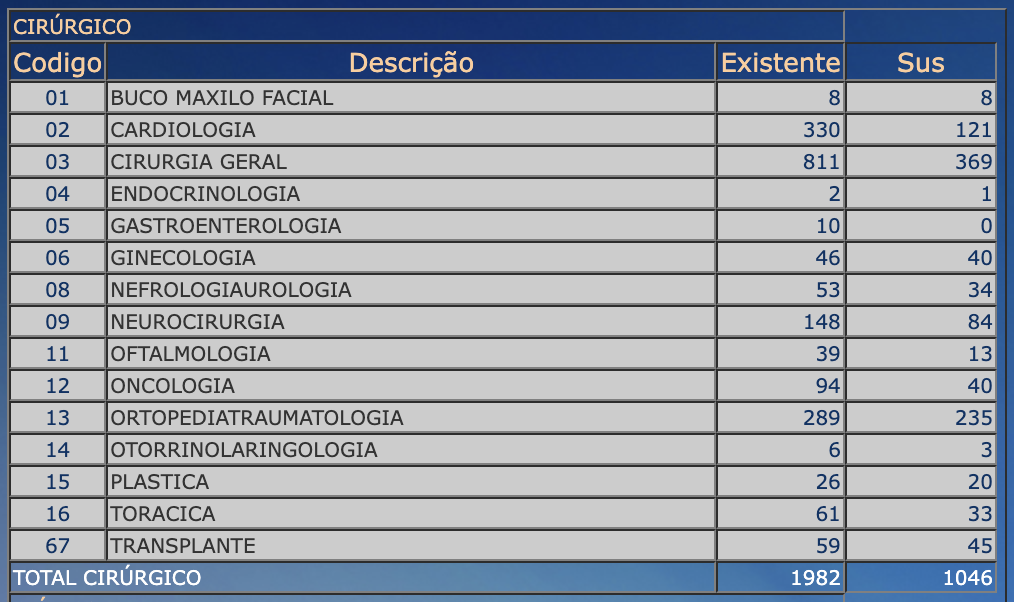
\includegraphics[width=\textwidth]{Capitulos/images/cnesnet1.png}
    \caption{Quantidade de leitos para especialidades do tipo ``cirúrgico'' nos hospitais de Porto Alegre/RS no mês de janeiro de 2024.}
    \label{fig:cnesnet1}
\end{figure}
%SO: sobre o caption da fig acima - colocar link dos dados. Fazer em todas as figs. (GV: revisar)

Para cada especialidade na lista, estão presentes informações sobre quais os hospitais que disponibilizam essa especialidade, a quantidade de leitos existentes e, dentre eles, quantos dos leitos são disponibilizados ao SUS, por fim, ao final da lista, apresenta-se o total de hospitais na cidade que disponibilizam essa especialidade de leito. A Figura~\ref{fig:cnesnet2} ilustra um exemplo dessas informações, onde a coluna ``CNES'' é o código identificador do cadastro do estabelecimento no sistema, ``Estabelecimento'' refere-se ao nome do hospital, ``Existente'' é a quantidade total de leitos para a especialidade e ``SUS'' é a quantidade de leitos SUS entre o número total de leitos.

\begin{figure}
    \centering
    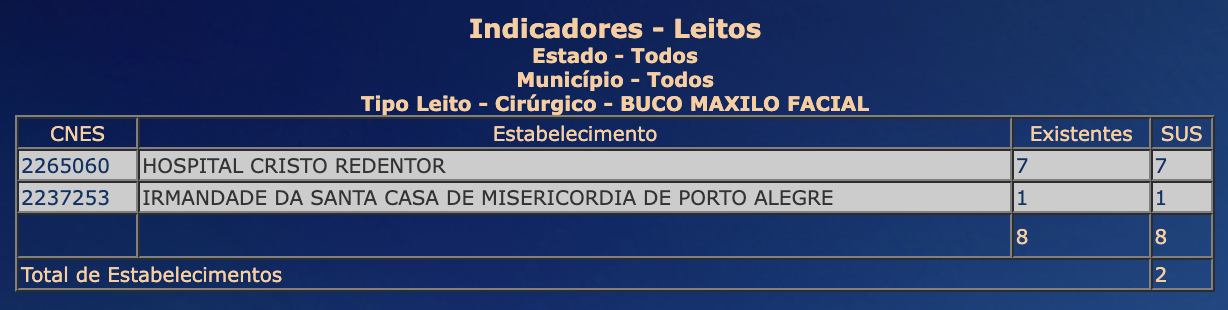
\includegraphics[width=\textwidth]{Capitulos/images/cnesnet2.png}
    \caption{Quantidade de leitos da especialidade ``Buco Maxilo Facial'' do tipo ``cirúrgico'' por hospital no mês de janeiro de 2024.}
    \label{fig:cnesnet2}
\end{figure}

Estes dados coletados serão utilizados como entradas em um conjunto de dados no qual cada hospital terá informações sobre suas especialidades por tipo de leito hospitalar. Após uma exploração nos dados disponíveis no CNESNet, foi decidido que, apesar de haver informações disponíveis sobre clínicas, nesta pesquisa consideraremos apenas os dados relacionados a hospitais, devido à baixa quantidade de leitos disponíveis e à complexidade de encontrar informações geográficas precisas sobre essas clínicas.

Por fim, a última etapa na coleta das informações para a criação do conjunto de dados ocorre na busca das coordenadas geográficas de cada hospital no Google Maps. É feita uma busca na ferramenta pelo nome do hospital (coluna ``Estabelecimento'' da Figura~\ref{fig:cnesnet2}) e recupera-se as informações de latitude e longitude de cada um deles. A Figura~\ref{fig:maps} mostra um exemplo da coleta desses dados utilizando o hospital São Lucas da PUCRS como referência, onde -30.05479 e -51.17142 são a latitude e longitude associadas, respectivamente.

\begin{figure}
    \centering
    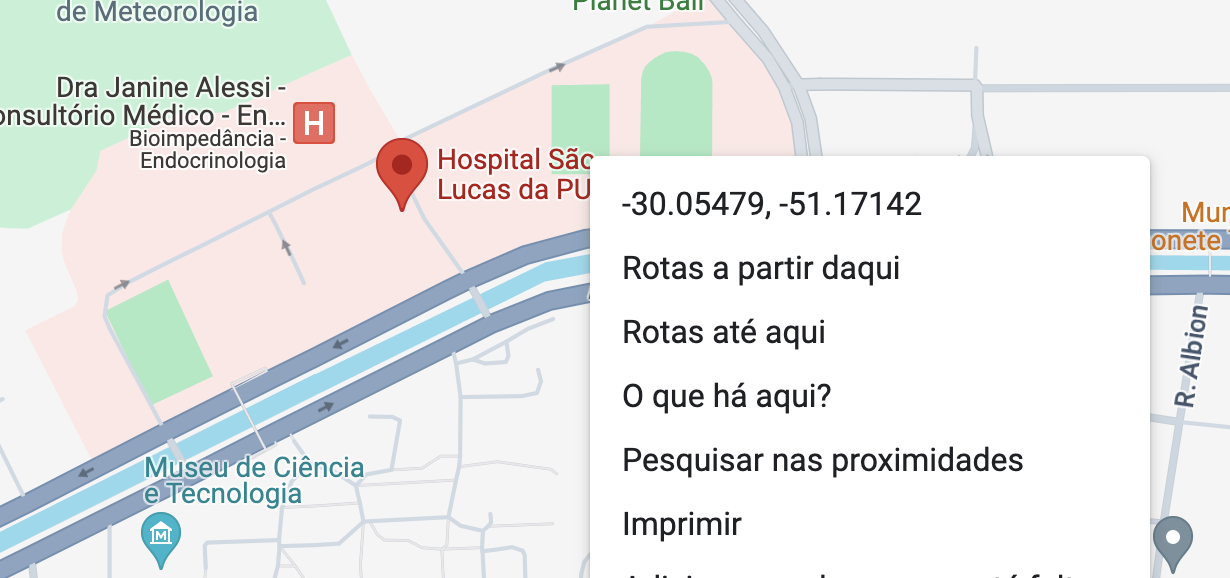
\includegraphics[width=0.97\textwidth]{Capitulos/images/maps.png}
    \caption{Busca pelas coordenadas geográficas de um hospital (latitude e longitude) no Google Maps.}
    \label{fig:maps}
\end{figure}

\section{Montagem do Conjunto de Dados}\label{sec:montagem_conjunto}
A montagem do conjunto de dados, representada na Figura~\ref{fig:metod}(b), é a etapa final na manipulação dos dados, etapa na qual ocorre a associação entre os dados recuperados nos endereços eletrônicos descritos na etapa anterior. O processo de montagem é realizado por meio da relação entre os dados dos hospitais e suas respectivas coordenadas. Para cada hospital recuperado no CNESNet, é associada uma coordenada no mapa (latitude e longitude), e as linhas do conjunto de dados são compostas pelas seguintes informações em um arquivo CSV:
%SO: coloquei em verbatim abaixo para ficar como dados de arquivo. coloca verbatim no parágrafo abauxo do item itemze em cada palavra
\begin{itemize}
    \item \begin{verbatim}LAT\end{verbatim}
    \item \begin{verbatim}LONG\end{verbatim}
    \item \begin{verbatim}HOSPITAL\end{verbatim}
    \item \begin{verbatim}REGIAO\end{verbatim}
    \item \begin{verbatim}DESCRICAO\end{verbatim}
    \item \begin{verbatim}TIPO\end{verbatim}
    \item \begin{verbatim}TOTAL\end{verbatim}
    \item \begin{verbatim}SUS\end{verbatim}
\end{itemize}
    
As colunas ``LAT'' e ``LONG'' referem-se às coordenadas geográficas de onde o hospital está localizado no mapa, ``HOSPITAL'' é o nome do hospital, ``REGIAO'' é o bairro onde o hospital está situado, ``DESCRICAO'' é a especialidade do leito do hospital, ``TIPO'' é o tipo de leito hospitalar, ``TOTAL'' é a quantidade total de leitos para a especialidade e ``SUS'' é a quantidade de leitos disponíveis para SUS entre o total de leitos. A Tabela~\ref{table:3} ilustra um exemplo dessa estrutura de entradas do conjunto de dados apresentando informações do hospital HPS. 
%SO: verbatim abaixo tb
\begin{table}[h!]
\centering
\begin{tabular}{ |c|c|c|c|c|c|c|c| } 
 \hline
 \verb|LAT| & \verb|LONG| & \verb|HOSPITAL| & \verb|REGIAO| & \verb|DESCRICAO| & \verb|TIPO| & \verb|TOTAL| & \verb|SUS|\\ 
 \hline
 \verb|-30.036...| & \verb|-51.211...| & \verb|HPS| & \verb|Bom Fim| & \verb|Cirurgia Geral| & \verb|Cirúrgico| & \verb|21| & \verb|21|\\  \hline
 \verb|-30.036...| & \verb|-51.211...| & \verb|HPS| & \verb|Bom Fim| & \verb|Neurocirurgia| & \verb|Cirúrgico| & \verb|15| & \verb|15|\\
 \hline
\end{tabular}
\caption{Exemplo de entradas do conjunto de dados criado.}
\label{table:3}
\end{table}

\subsection{Análise do Conjunto de Dados}
Concluída a etapa de montagem do conjunto de dados, os dados estão prontos para serem utilizados na pesquisa. Para isso, inicialmente utilizamos a aplicação web Jupyter Notebook\footnote{\url{https://docs.jupyter.org/en/latest/}} disponível através do Google Colab\footnote{\url{https://colab.research.google.com/}} %SO: link (FEITO)
para a realização de uma análise sobre os dados e entender a distribuição das informações dos hospitais no conjunto de dados. O desenvolvimento da exploração e análise dos dados foi realizado utilizando a linguagem Python\footnote{\url{https://docs.python.org/3/}}, juntamente com a biblioteca de manipulação e análise de dados Pandas\footnote{\url{https://pandas.pydata.org/docs/}}, dentro da aplicação web Jupyter Notebook, uma aplicação web utilizada para criar e compartilhar documentos computacionais~\cite{JUPYTER}. 

O conjunto de dados final resultou em um arquivo contendo 254 entradas, cada uma representando informações de leitos hospitalares para uma determinada especialidade, conforme apresentado anteriormente. Foram recuperadas ao todo informações de 28 hospitais no CNESNet, distribuídos em 22 bairros de Porto Alegre, abrangendo um total de 48 especialidades de leitos distintos. Além disso, foram identificados 7 tipos de leitos distintos (``cirúrgico'', ``clínico'', ``obstétrico'', etc.). Ao total, estão disponíveis informações de 7.529 leitos hospitalares, dos quais 4.689 leitos estão disponíveis para o SUS, representando aproximadamente 62,27\% dos leitos dos hospitais selecionados.

No gráfico da Figura~\ref{fig:graph1}, destacam-se os 10 hospitais com as maiores diversidades de especialidades de leitos. Entre eles, os hospitais com o maior número de especialidades distintas são o Hospital Nossa Senhora da Conceição, a Irmandade da Santa Casa de Misericórdia de Porto Alegre e o Hospital Divina Providência, contendo 31, 30 e 24 especialidades de leitos, respectivamente.

\begin{figure}
    \centering
    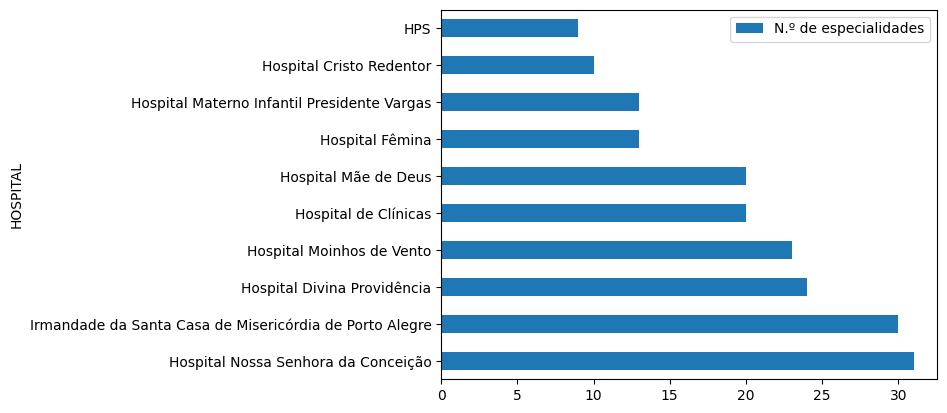
\includegraphics[width=\textwidth]{Capitulos/images/graph1.png}
    \caption{Os 10 hospitais selecionados com o maior número de especialidades distintas.}
    \label{fig:graph1}
\end{figure}

Já os 10 hospitais com os maiores números de leitos disponíveis (Figura~\ref{fig:graph2}) são a Irmandade da Santa Casa de Misericórdia de Porto Alegre, com 1.066 leitos, o Hospital Nossa Senhora da Conceição, com 912, e o Hospital de Clínicas, com 885 leitos disponíveis. Observando a Figura~\ref{fig:graph2}, em termos de quantidade de leitos SUS, os hospitais Nossa Senhora da Conceição, com 912 leitos, Hospital de Clínicas, com 747, e Associação Hospitalar Vila Nova, com 637, são os que possuem maior disponibilidade para leitos públicos. De maneira geral, os leitos hospitalares tem uma disponibilidade equilibrada entre privados e SUS. No entanto, observa-se a presença de hospitais que não oferecem atendimento SUS, como os hospitais Mãe de Deus, Ernesto Dornelles e Moinhos de Vento. Além disso, há hospitais que têm toda ou a maior parte de sua capacidade dedicada ao SUS, como o Hospital de Clínicas, com cerca de 84\%, a Associação Hospitalar Vila Nova, com cerca de 99\% de sua capacidade, e o hospital Nossa Senhora da Conceição, com 100\% da capacidade dedicada.

\begin{figure}
    \centering
    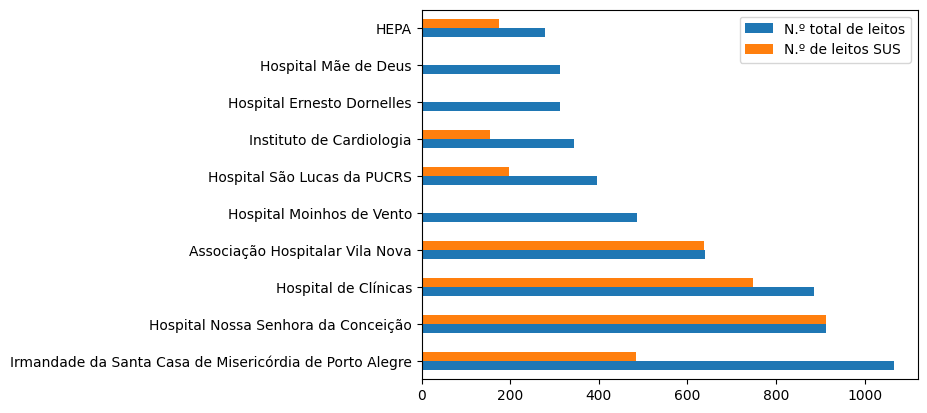
\includegraphics[width=\textwidth]{Capitulos/images/graph2.png}
    \caption{Os 10 hospitais selecionados com o maior número de leitos, separados entre total e SUS.}
    \label{fig:graph2}
\end{figure}

Seguindo a análise do conjunto de dados, a Figura~\ref{fig:graph3} apresenta as 10 especialidades mais frequentes nos leitos dos hospitais de Porto Alegre. As especialidades de ``Cirurgia Geral'', do tipo ``Cirúrgico'', e ``Clínica Geral'', do tipo ``Clínico'', são as mais comuns nos hospitais da cidade, presentes em 18 hospitais cada. Em seguida, a especialidade ``UTI Adulto - Tipo III'', do tipo de leito ``Complementar'', está presente em 12 hospitais dos 28 hospitais selecionados.

\begin{figure}
    \centering
    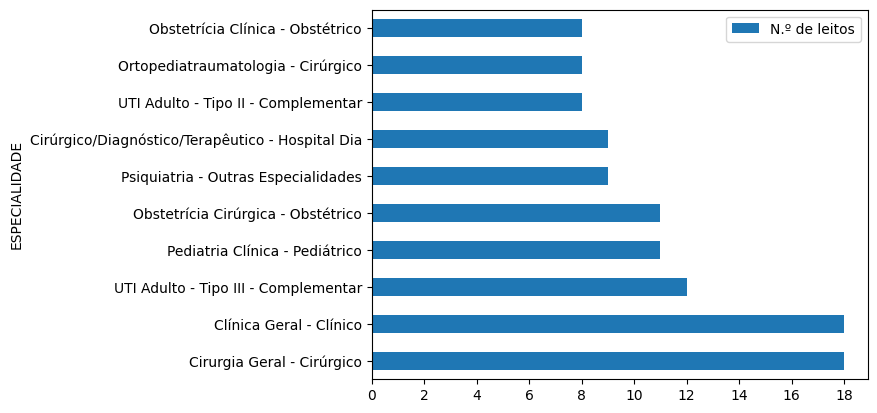
\includegraphics[width=\textwidth]{Capitulos/images/graph3.png}
    \caption{As 10 especialidades mais frequentes nos leitos dos hospitais selecionados.
    %GA: Os dados não tem falores float, certo? caso não, ajustar o exito X para ser valores inteiros (GV: corrigido)
    }
    \label{fig:graph3}
\end{figure}

Feitas as análises que complementam a busca e o armazenamento estruturado dos dados, parte-se para a apresentação dos processo de interação e simulação.

\section{Interface de Configuração}\label{sec:interface_config}
A interface gráfica de configuração (representada na Figura~\ref{fig:metod}(c))
%SO: conferir se é mesmo (c). quando falar das partes da fig1, mencionar a letrinha (GV: revisar)
neste estudo foi desenvolvida com o objetivo de facilitar a parametrização dos dados de entrada do modelo de simulação. Além disso, espera-se tornar o uso do simulador mais acessível para pessoas de fora da área da tecnologia, eliminando a necessidade do usuário de criar arquivos em formatos comuns para profissionais de computação, como por exemplo JSON e CSV.

A tecnologia central empregada no desenvolvimento da interface foi o Flask\footnote{\url{https://flask.palletsprojects.com/en/3.0.x/}}, um \textit{framework} escrito em Python voltado para o desenvolvimento web. Essa tecnologia é crucial para estabelecer a conexão entre os parâmetros do usuário e a execução do LODUS a partir deles. Além disso, outras tecnologias foram utilizadas no desenvolvimento da interface. Utilizamos HTML, CSS e Bootstrap\footnote{\url{https://getbootstrap.com/docs/4.6/getting-started/introduction/}} para estilizar a interface e tornar sua utilização amigável, JavaScript para auxiliar na lógica de programação e também na conexão com o código do LODUS, e o Plotly\footnote{\url{https://plotly.com/}
} na apresentação dos resultados da simulação utilizando um mapa \textit{choropleth}. As tecnologias utilizadas no estudo foram selecionadas devido à familiaridade dos pesquisadores.

A interface foi desenvolvida para abranger três funcionalidades principais: permitir a configuração dos parâmetros do modelo de simulação, possibilitando o uso de dados reais de hospitais provenientes do DATASUS\footnote{\url{https://datasus.saude.gov.br/}}, disponíveis no CNESNet ou que o usuário crie dados fictícios, facilitando a execução do simulador para diversos tipos de usuários; apresentar os resultados obtidos na simulação de forma clara e objetiva; e permitir que o usuário escolha especialidades de leitos para a geração de textos no contexto desejado. Nesta seção, será abordada a etapa de configuração dos parâmetros do modelo de simulação.

Para que o usuário fosse capaz de configurar a parametrização do modelo de simulação, foi criada uma interface (Figura~\ref{fig:simul1}) que permite a entrada de parâmetros como o título da simulação (Figura~\ref{fig:simul1}(a)), período de simulação em dias e horas (Figura~\ref{fig:simul1}(b)), os quais serão contabilizados como passos de simulação, 
%SO: ficou essa troca? (GV: corrigido)
escolha ou criação de hospitais a serem simulados (Figura~\ref{fig:simul1}(c)), e a listagem dos hospitais selecionados (Figura~\ref{fig:simul1}(d)), possibilitando a configuração e remoção de cada um deles.

\begin{figure}
    \centering
    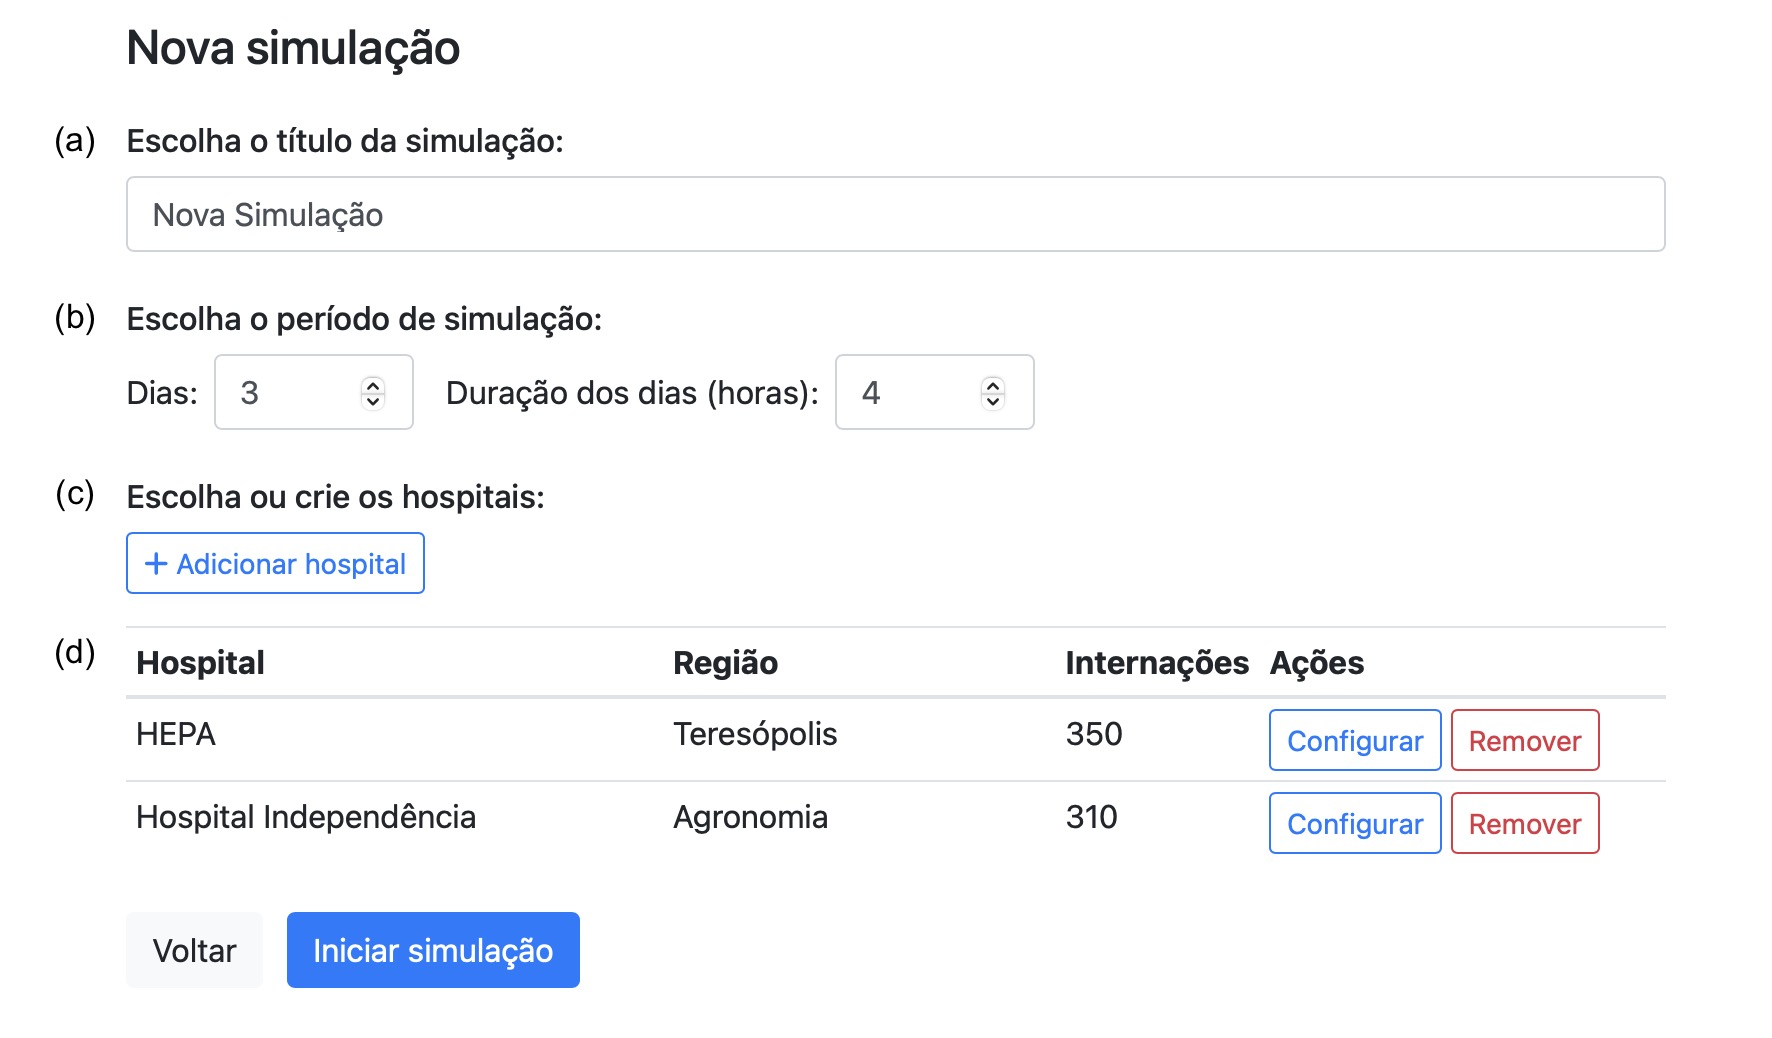
\includegraphics[width=\textwidth]{Capitulos/images/simul1.jpeg}
    \caption{Tela de configuração dos parâmetros de simulação.}
    \label{fig:simul1}
\end{figure}

Ao usuário selecionar a opção ``Adicionar hospital'' (Figura~\ref{fig:simul1}(c)), aparecem opções de parametrização relacionadas à criação ou seleção de um hospital a ser utilizado na simulação. Nessa tela (Figura~\ref{fig:simul2}), o usuário pode escolher um hospital a partir de dados provenientes do conjunto de dados apresentado na seção anterior (Figura~\ref{fig:simul2}(a)), ou criar um novo hospital (Figura~\ref{fig:simul2}(b)), adicionar especialidades de leitos a partir dos dados do CNESNet (Figura~\ref{fig:simul2}(c)), criar uma nova especialidade (Figura~\ref{fig:simul2}(d)), ou listar as especialidades selecionadas com a possibilidade de remover as indesejadas (Figura~\ref{fig:simul2}(e)).

\begin{figure}
    \centering
    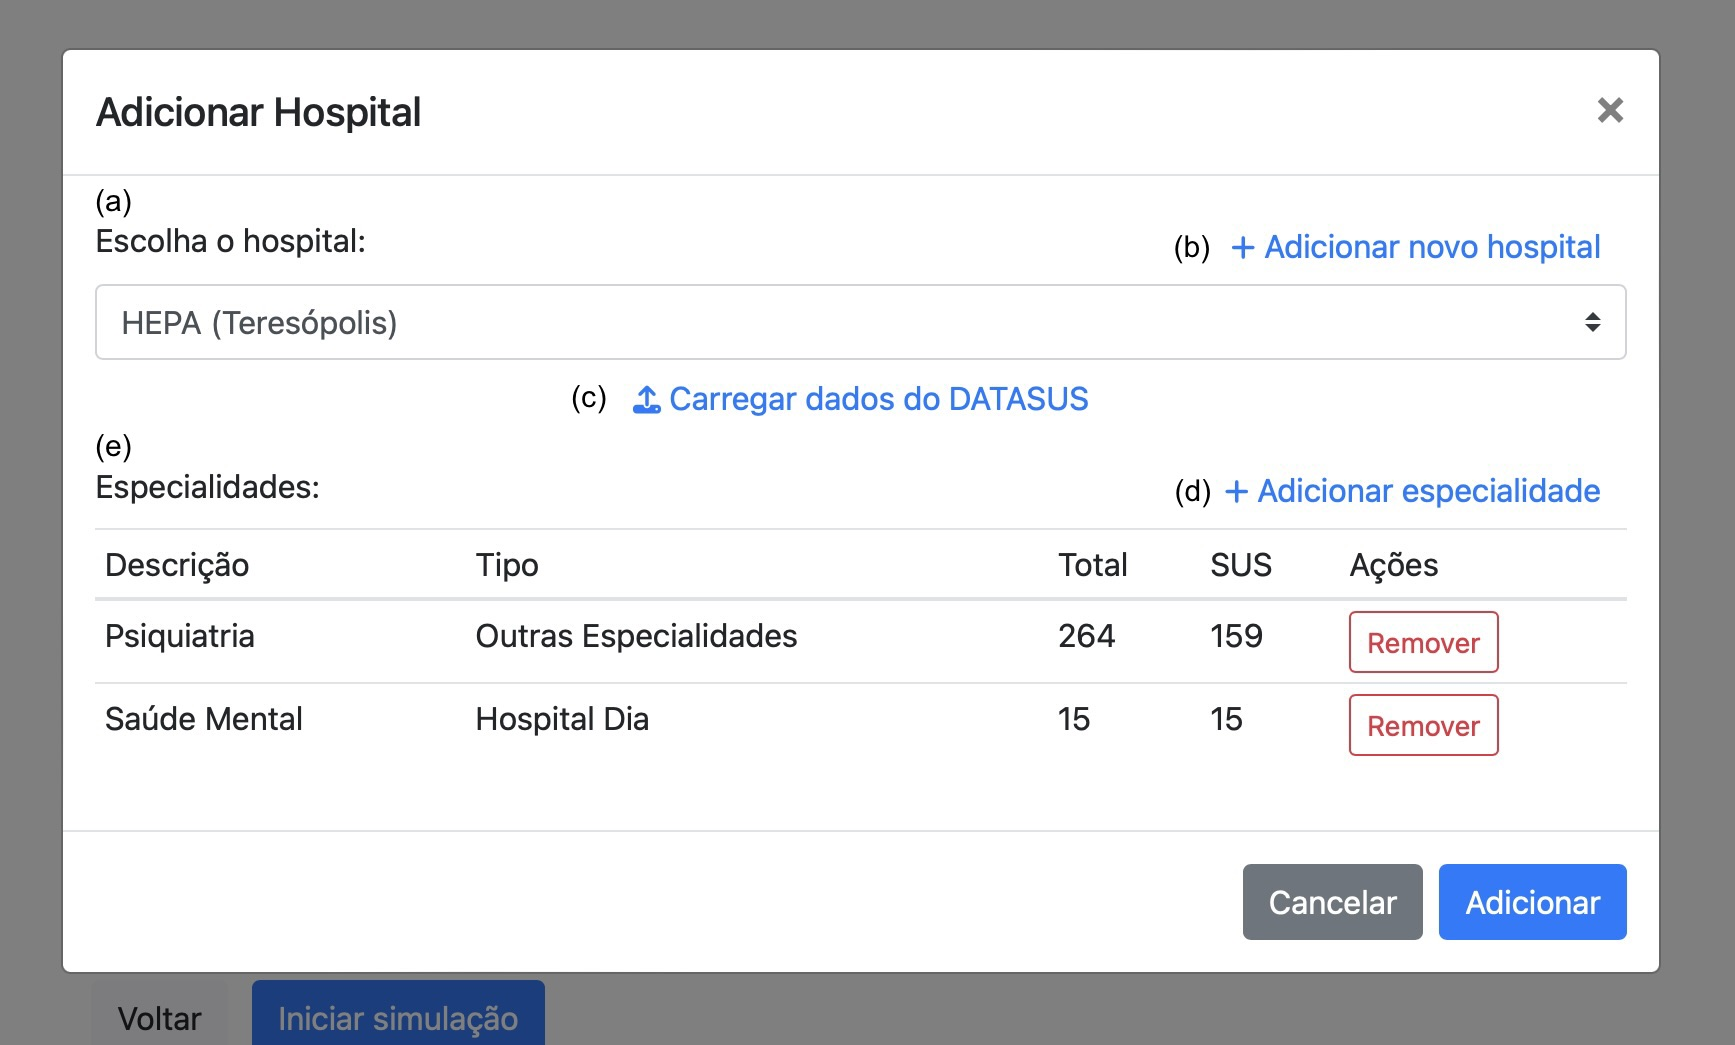
\includegraphics[width=\textwidth]{Capitulos/images/simul2.jpeg}
    \caption{Tela de seleção de hospital um hospital para a simulação.}
    \label{fig:simul2}
\end{figure}

Ao selecionar ``Adicionar novo hospital'' (Figura~\ref{fig:simul2}(b)), o usuário tem a opção de inserir um novo hospital para escolha na configuração da simulação (Figura~\ref{fig:simul3}), para isso, o usuário deve informar o nome do hospital (Figura~\ref{fig:simul3}(a)), selecionar a região (bairro) à qual ele pertence (Figura~\ref{fig:simul3}(b)) e definir as coordenadas geográficas (latitude e longitude) do mesmo (Figura~\ref{fig:simul3}(c)).

\begin{figure}
    \centering
    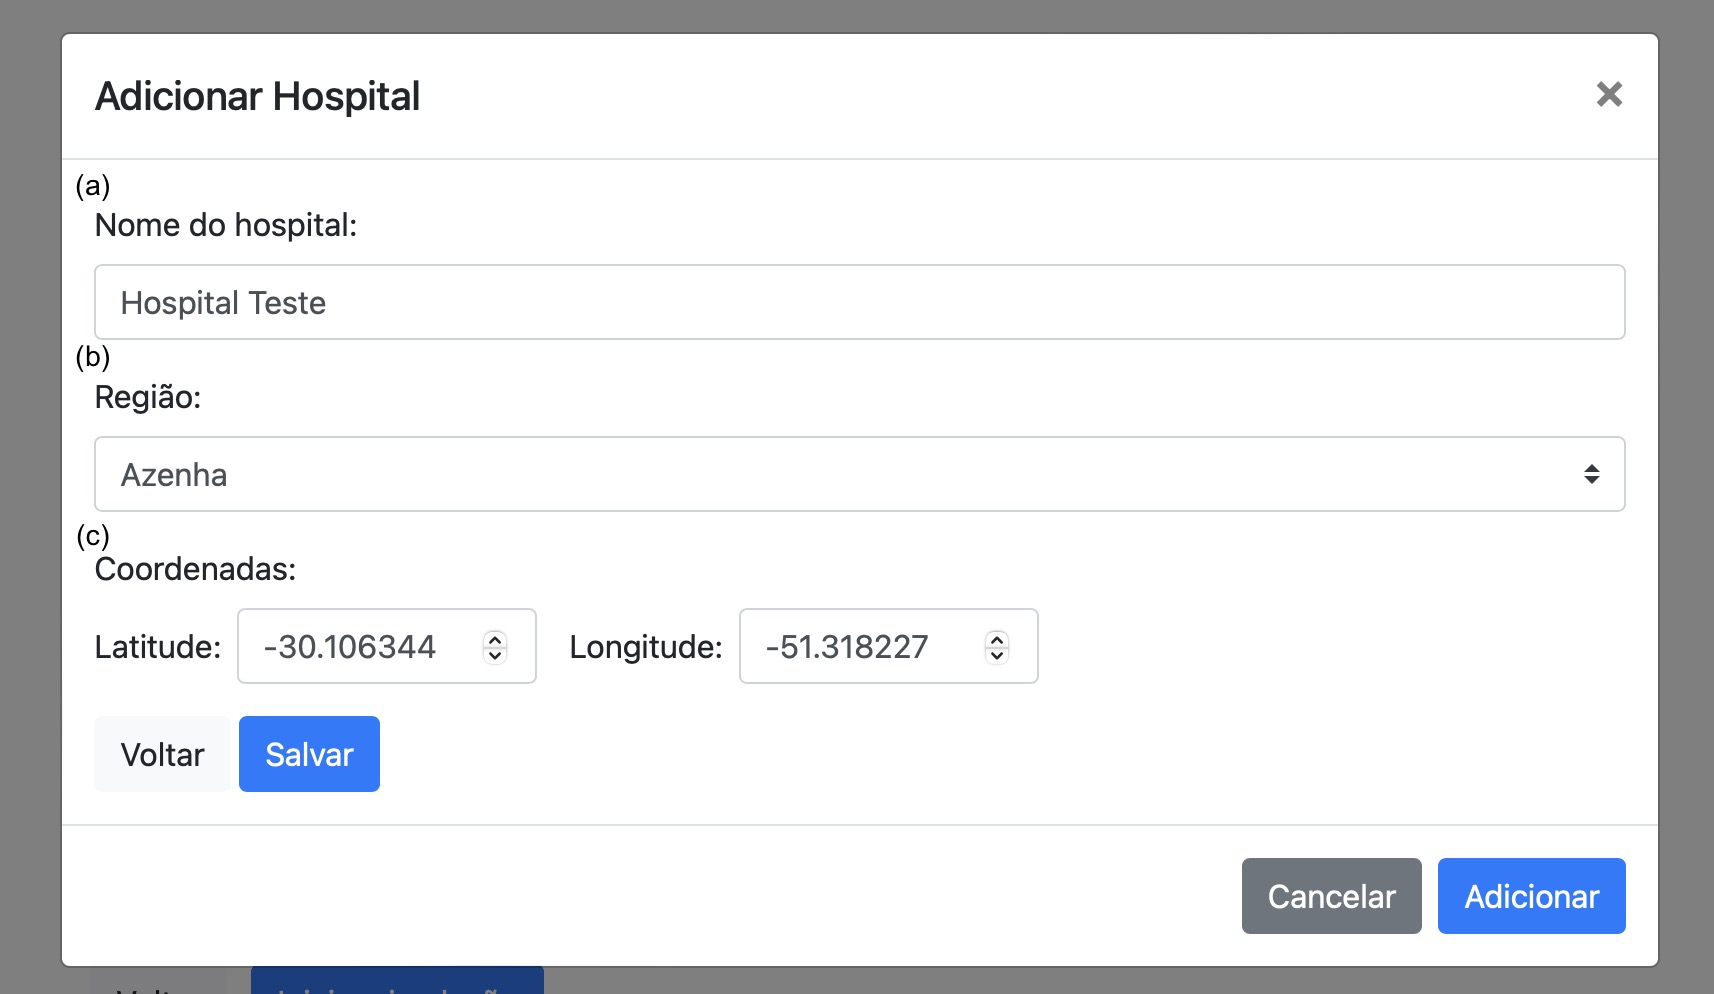
\includegraphics[width=\textwidth]{Capitulos/images/simul3.jpeg}
    \caption{Tela de criação de uma opção de hospital para a simulação.}
    \label{fig:simul3}
\end{figure}

Após a seleção ou criação de um hospital, o usuário pode personalizar suas características, podendo selecionar diversas especialidades dentre as já existentes ou criar uma nova especialidade de leito customizada (Figura~\ref{fig:simul4}). Para isso, deve-se informar o nome da especialidade (Figura~\ref{fig:simul4}(a)). Se ela já existir, o usuário seleciona na lista; caso contrário, deve-se informar o nome, o tipo de leito (Figura~\ref{fig:simul4}(b)), e a quantidade total de leitos disponíveis e dentre os leitos disponíveis, a quantidade dedicada para o SUS (Figura~\ref{fig:simul4}(c)).

\begin{figure}
    \centering
    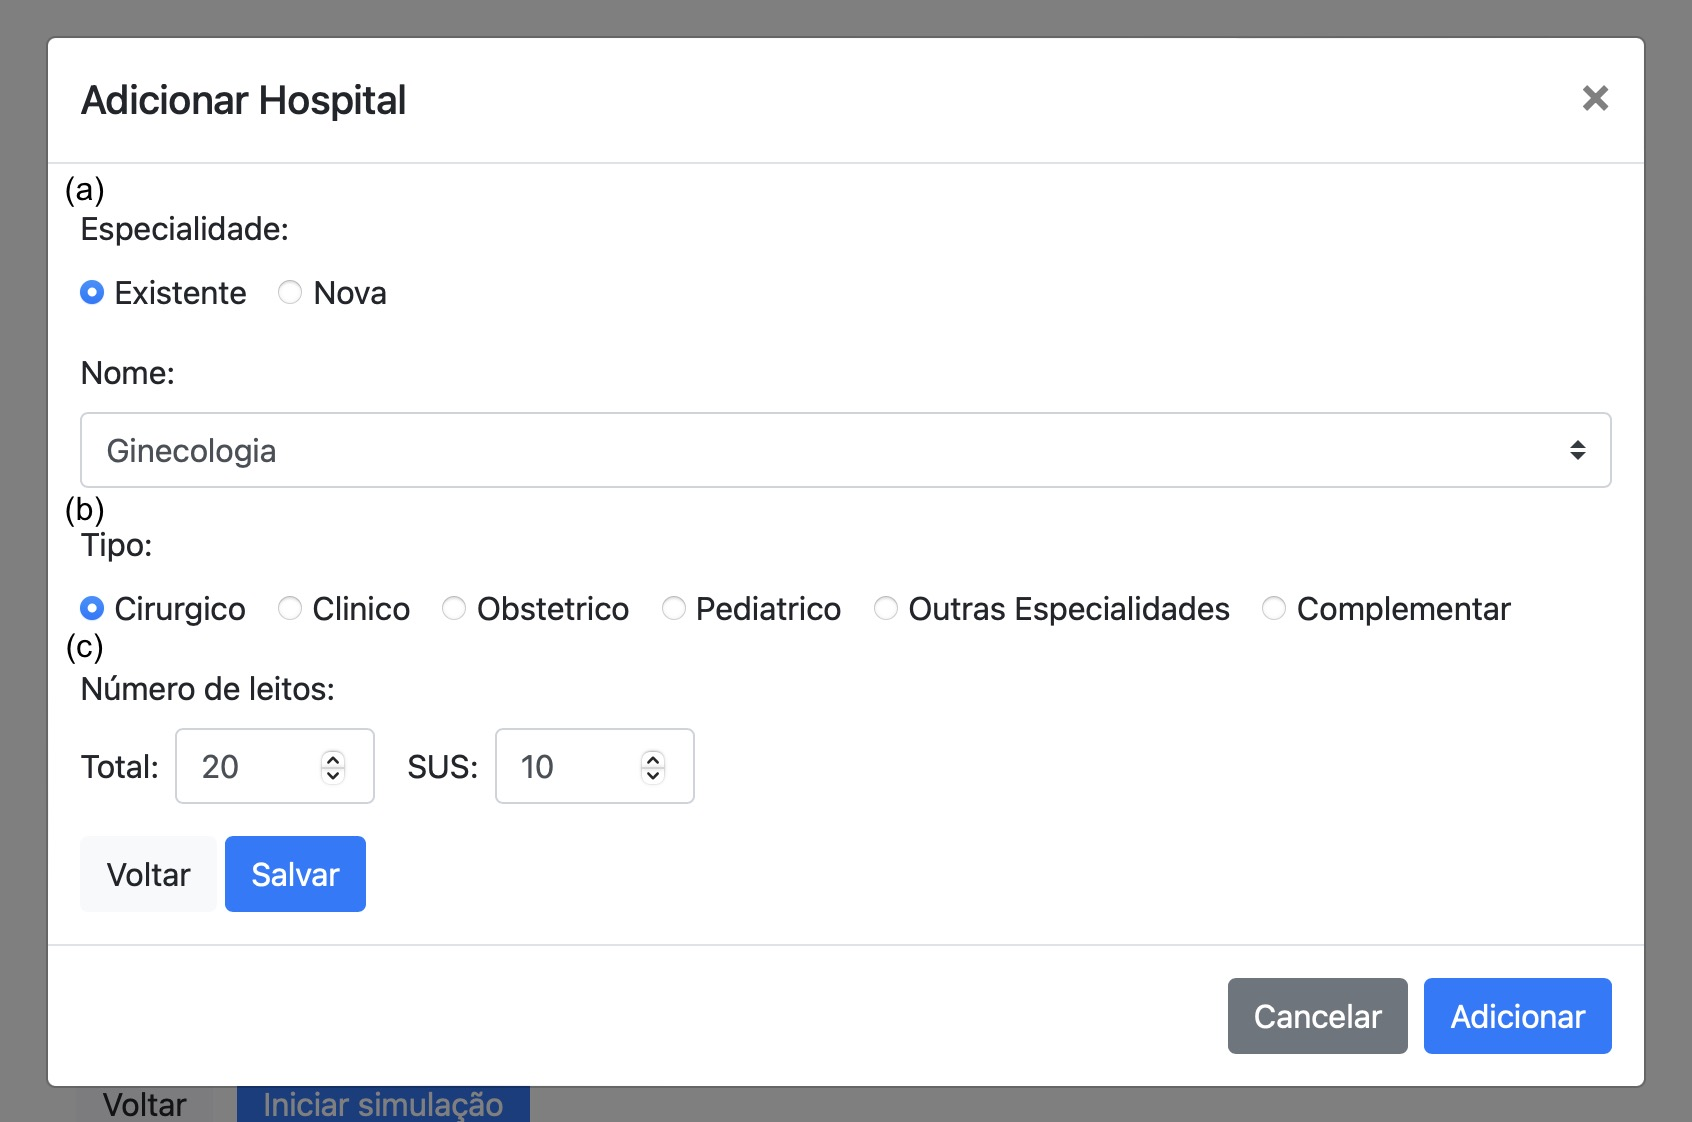
\includegraphics[width=\textwidth]{Capitulos/images/simul4.jpeg}
    \caption{Tela de criação de uma especialidade.}
    \label{fig:simul4}
\end{figure}

Por fim, a última ação do usuário na criação dos parâmetros de simulação é a definição das chamadas de pacientes para hospitais na simulação (Figura~\ref{fig:simul5}). Informa-se quantos pacientes serão internados para uma especialidade específica no período de simulação definido na tela inicial (Figura~\ref{fig:simul5}(a)), quantas internações serão destinadas ao SUS (Figura~\ref{fig:simul5}(b)) e por quantos passos de simulação, em média, os internados naquela especialidade permanecem no leito hospitalar na simulação, definindo o número mínimo e máximo de passos (Figura~\ref{fig:simul5}(c)). Por exemplo, na Figura~\ref{fig:simul5}, o hospital HEPA possui 264 leitos da especialidade ``Psiquiatria'' do tipo ``Outras Especialidades'', sendo 159 deles disponíveis para o SUS. Foi informado que durante o período de simulação serão utilizados 500 leitos para pacientes, sendo 300 em leitos do SUS. Também foi parametrizado que um paciente pode permanecer em média de 1 a 4 passos de simulação ocupando o leito.

\begin{figure}
    \centering
    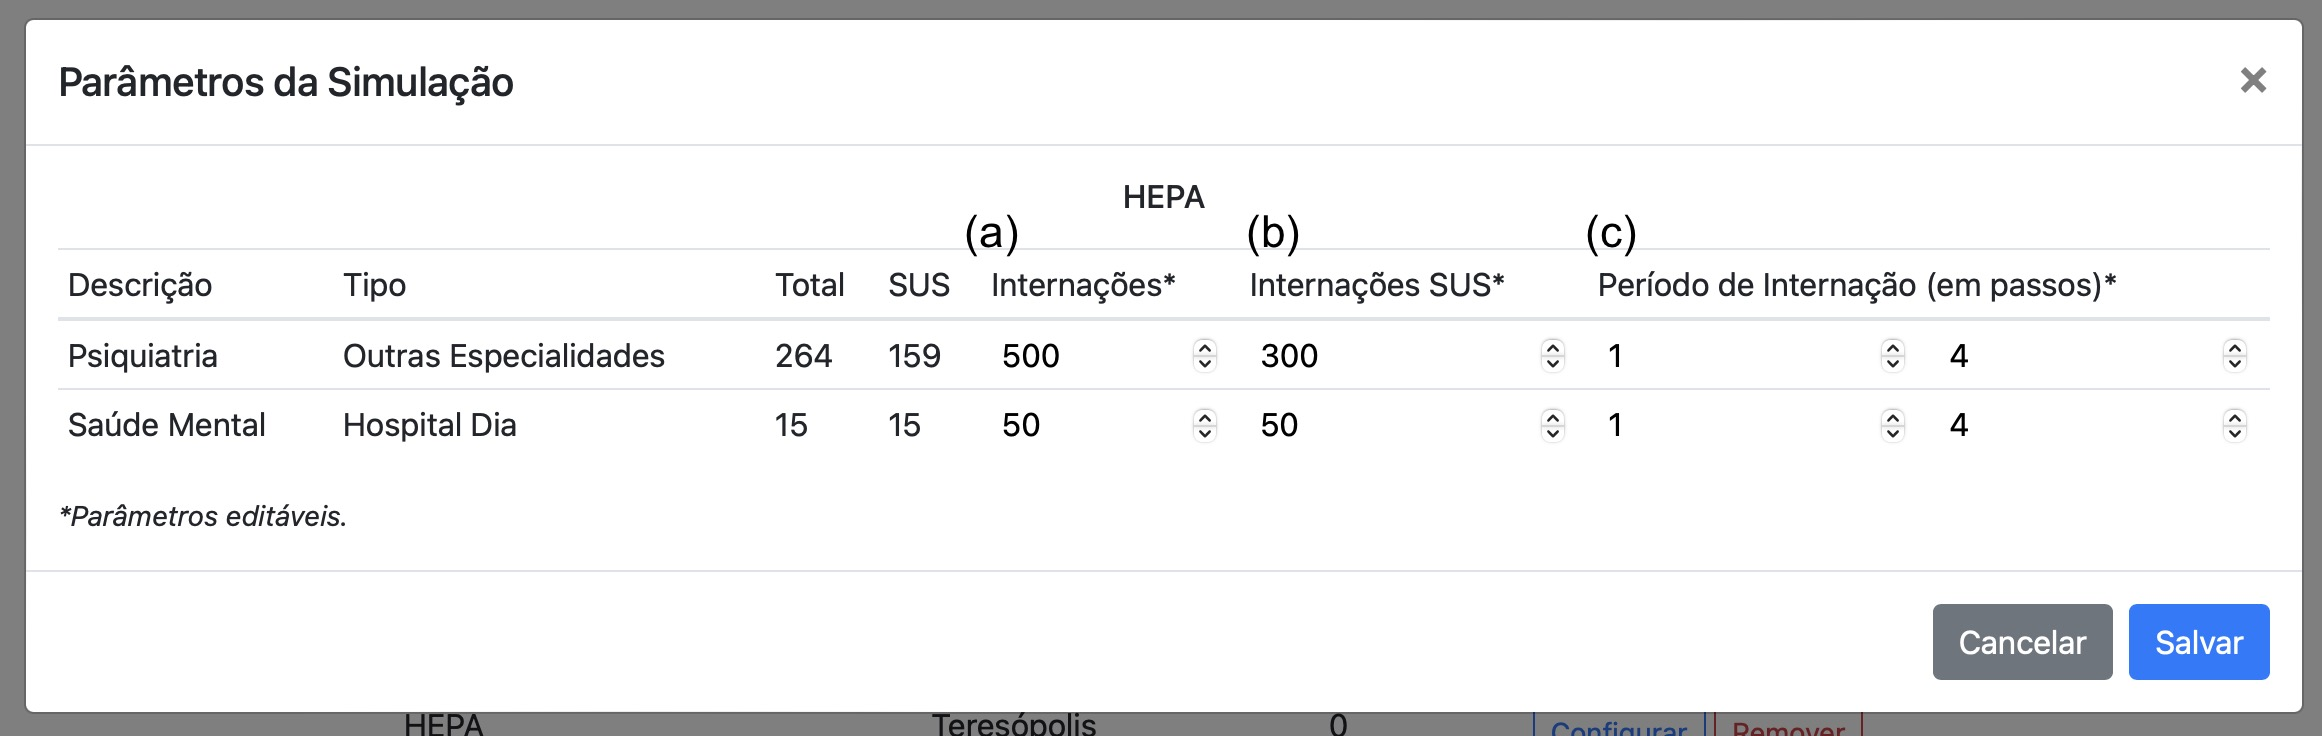
\includegraphics[width=\textwidth]{Capitulos/images/simul5.jpeg}
    \caption{Tela de parametrização da simulação.}
    \label{fig:simul5}
\end{figure}

Finalmente, ao clicar no botão "Iniciar simulação", é gerado um arquivo JSON a ser utilizado como entrada do modelo de simulação a partir dos parâmetros configurados na interface gráfica. Inicia-se a execução do modelo de simulação e, após o término da execução, os resultados são apresentados. A Seção~\ref{sec:visualizacao_resultados} deste capitulo detalha a interface utilizada para apresentar os resultados do modelo. A Listagem~\ref{json-model} ilustra um exemplo da estrutura do arquivo JSON gerado pela etapa de parametrização do modelo. 
%SO: no listing tem que ser colocadas letrinhas (a)(b) e explicada todo o texto (GV: revisao)

\begin{listing}
\begin{minted}[frame=single,
               framesep=3mm,
               linenos=true,
               xleftmargin=21pt,
               tabsize=4]{js}
{
    "title": "Nova simulação",
    "days": 3,
    "day_duration": 4,
    "hospital_data": [
        {
            "name": "HEPA",
            "region": "Teresópolis",
            "latitude": -30.0871043,
            "longitude": -51.2089115,
            "specialties": [
                {
                    "name": "Psiquiatria",
                    "sectors": [
                        {
                            "type": "Outras Especialidades",
                            "total": "264",
                            "sus": "159"
                        }
                    ]
                },
                ...
            ]
        }
        ...
    ],
    "hospital_calls": [
        {
            "name": "HEPA",
            "total-calls": [
                {
                    "name": "Psiquiatria",
                    "type": "Outras Especialidades",
                    "admissions": "20",
                    "admissions-sus": "20",
                    "range-start": "1",
                    "range-end": "3"
                },
                ...
            ]
        }
        ...
    ]
}
\end{minted}
\caption{Exemplo arquivo JSON de entrada do modelo de simulação gerado pela interface.} 
\label{json-model}
\end{listing}
\pagebreak

O arquivo representado pela Listagem~\ref{json-model} é composto das informações a seguir. O campo ``\textit{title}'' está associado ao titulo da simulação, ``\textit{days}'' é a duração da simulação em dias, ``\textit{day\_duration}'' a duração de um dia na simulação em horas, ``\textit{hospital\_data}'' contém as informações parametrizadas relacionadas a capacidade dos leitos hospitalares de cada hospital selecionado e ``\textit{hospital\_calls}'' contém as informações relacionadas ao fluxo de pacientes nos leitos hospitalares da simulação.

\section{Plugin do LODUS}\label{sec:plugin_lodus}
A partir dos dados informados e descritos nas seções anteriores, a presente etapa apresenta o desenvolvimento de um 
\textit{plugin} para o \textit{framework} LODUS~\cite{9239083}. 
%SO: ref ao lodus (GV: corrigido)
O objetivo desse \textit{plugin} é adicionar à aplicação a capacidade de contextualizar o ambiente de simulação urbana virtual para casos de ocupação de leitos hospitalares, parte fundamental no desenvolvimento da ferramenta LODUS-Health.
%SO: acima - plugin em itálico (GV: corrigido)

Para iniciar a execução da simulação, o LODUS necessita de um arquivo de configuração com a estrutura previamente definida pelos autores do \textit{framework}, o qual pode ser alterado em ferramentas de edição de texto. Entretanto, o propósito deste trabalho também é evitar a necessidade de realizar alterações nos arquivos utilizando ferramentas de edição de texto antes da execução da simulação. Para isso, a configuração do ambiente é realizada combinando os dados dos dois arquivos necessários para a contextualização e execução. Nesse processo, utiliza-se a linguagem Python. A Listagem~\ref{input-file} abaixo demonstra um exemplo da estrutura do arquivo requisitado pela aplicação, onde, ``\textit{population\_template}'' está atribuído a uma definição de características comuns entre toda a população no modelo de simulação, ``\textit{repeating\_global\_actions}'' as ações que ocorrem na simulação em determinados períodos, ``\textit{regions}'' as configurações dos bairros da cidade dentro da simulação contendo informações como, posição geográfica, as regiões vizinhas mais próximas e os pontos de interesse dentro da região contendo informações geográficas e o tamanho da população naquele ponto.

%SO: tens que colocar (a)(b) no arquivo abaixo e explicar o listing. (GV: revisao)

\begin{listing}
\begin{minted}[frame=single,
               framesep=3mm,
               linenos=true,
               xleftmargin=21pt,
               tabsize=4]{js}
{
  "population_template": {
    "traceable_properties": {},
    "sampled_properties": {}
  },
  "repeating_global_actions": [],
  "regions": [
    {
      "name": "Independência",
      "long_lat_position": [-51.2114165227445, -30.0283138642156]
      "neighbors": [
        "Floresta",
        "Moinhos de Vento",
        ...
      ],
      "nodes": {
        "home": {
          "characteristics": {
            "long_lat_position": [-51.209426628695, -30.028013704038]
          },
          "population_groups": [
            {
              "size": 8112,
              "traceable_properties": {},
              "description": {}
            }
          ],
          "time_actions": {}
        }
      }
    }...
  ]
}

\end{minted}
\caption{Exemplo de arquivo de configuração para execução do \textit{framework} LODUS.} 
\label{input-file}
\end{listing}

Os dados de configuração dos parâmetros definidos pelo usuário na interface de configuração, apresentados na seção anterior, são incorporados à configuração do ambiente de simulação, juntamente com os dados deste arquivo necessário para a execução do ambiente de simulação. O primeiro passo dessa tarefa é a configuração dos passos de simulação, que consiste na multiplicação entre a quantidade de dias a serem simulados e a duração do dia parametrizados pelo usuário. Uma configuração de 4 dias e com 3 de duração resulta em 12 passos de simulação, por exemplo.

Seguindo na configuração do \textit{plugin}, o próximo passo é a configuração dos pontos de interesse dentro da simulação, sendo um ponto de interesse uma área dentro do ambiente de simulação na qual os grupos podem se deslocar. Para cada região, optamos por trabalhar com dois possíveis pontos de interesse na simulação, sendo eles casas e hospitais. Para ilustrar, grupos de um ou mais pacientes saem de suas casas para serem internados nos hospitais, e pacientes deixam hospitais para retornarem para suas casas após um determinado período de internação. Neste estudo, não estamos considerando que pacientes venham de outros possíveis pontos de interesse ou que venham a óbito no hospital; somente o controle do fluxo de internações é considerado, pacientes que venham a óbito ou recebam alta hospitalar são tratados apenas como uma desocupação do leito hospitalar. Para que um hospital seja reconhecido como um ponto de interesse, cada hospital selecionado no arquivo de configuração é manipulado de tal forma a ser considerado um ``nodo'' dentro de uma região, sendo ``nodos'', pontos de interesse dentro de uma região com suas características próprias. Ao final dessa junção entre os dados das duas fontes, internamente na aplicação, um ``nodo'' que caracteriza um hospital dentro de uma região possui a seguinte estrutura representada na Listagem~\ref{nodo-structure}:

\begin{listing}
\begin{minted}[frame=single,
               framesep=3mm,
               linenos=true,
               xleftmargin=21pt,
               tabsize=4]{js}     
{
    "name": "HEPA",
    "id": "5",
    "routine": {
        "name": "None",
        "actions": {}
    },
    "characteristics": {
        "long_lat_position": [
            -51.2089115,
            -30.0871043
        ],
        "hospital_bed": {
            "config": [
                {
                    "name": "Psiquiatria",
                    "sectors": [
                        {
                            "type": "Outras Especialidades",
                            "total": "264",
                            "sus": "159"
                        }
                    ]
                }...
            ],
            "calls": [
                {
                    "name": "Psiquiatria",
                    "type": "Outras Especialidades",
                    "admissions": "20",
                    "admissions-sus": "20",
                    "range-start": "1",
                    "range-end": "4",
                    "distribution": [0, 0, ..., 0],
                    "distribution-sus": [6, 2, 0, ..., 1]
                },
            ]
        }
    },
    "blobs": []
}
\end{minted}
\caption{Exemplo da estrutura interna de um nodo dentro do modelo de simulação.} 
\label{nodo-structure}
\end{listing}

A Listagem~\ref{nodo-structure} apresenta as informações que caracterizam um hospital dentro do ambiente de simulação. O campo ``\textit{name}'' refere-se ao nome do hospital, ``\textit{id}'' é um identificador único para o nodo, ``\textit{routine}'' mostra as rotinas associadas ao hospital, e ``\textit{characteristics}'' são as características que compõem o nodo, incluindo ``\textit{long\_lat\_position}'' para a posição geográfica do hospital no mapa, ``\textit{hospital\_bed}'' para as configurações de leitos do hospital, onde ``\textit{config}'' são as configurações de disponibilidade de leitos e ``\textit{calls}'' refere-se às configurações de ocupação dos leitos. O campo ``\textit{config}'' está associado a uma lista de especialidades do hospital. No exemplo, o hospital HEPA possui a especialidade ``Psiquiatria'' e o tipo de leito (\textit{sectors}) ``Outras Especialidades'', totalizando 264 leitos, sendo 159 do SUS. Em ``\textit{calls}'', há uma lista de status de ocupação dos leitos. Para a especialidade ``Psiquiatria'' do tipo ``Outras Especialidades'', serão 20 pacientes internados no período de simulação (\textit{admissions}), sendo 20 internados nos leitos SUS (\textit{admissions-sus}). Cada paciente ficará no hospital por um período de 1 a 4 passos de simulação (\textit{range-start} e \textit{range-end}). Os campos ``\textit{distribution}'' e ``\textit{distribution-sus}'' são listas do tamanho do número total de passos de simulação, onde cada índice da lista representa uma entrada de pacientes para aquele leito no passo de execução atual. Por exemplo, no passo de simulação 0, 6 pacientes chegam no leito SUS e no passo 1, chegam 2. Por fim, ``\textit{blobs}'' é a lista de grupos naquele nodo, ou seja, os grupos de pacientes que estão naquele hospital com suas características próprias.

A última etapa antes da execução da simulação é a configuração das ``\textit{repeating actions}''. Uma \textit{repeating action} é uma ação que o modelo de simulação executa em um período único ou em intervalos determinados. Para cada passo de execução, são definidos três tipos de ações no \textit{plugin}: ``\textit{patient\_call}'', ``\textit{patient\_distribution}'' e ``\textit{patient\_discharge}''. Na ação ``\textit{patient\_call}'', é feita a chamada de pacientes para dentro do hospital, ou seja, um grupo de pacientes sai de suas casas para ocuparem leitos hospitalares, a única condições de busca de pacientes é que sejam apenas os que ainda não tenham sido encaminhados a algum dos hospitais na simulação. A ação ``\textit{patient\_distribution}'' transforma o grupo de pacientes que chegaram ao hospital em pacientes individuais e atribui-se cada paciente a um leito hospitalar. Já a ação ``\textit{patient\_discharge}'' é responsável por desocupar os leitos hospitalares; ao executar a ação, o hospital remove os pacientes dos leitos e os retorna cada um para sua casa em sua região de origem, utilizando uma ação previamente disponível no \textit{framework} ``\textit{move\_population}''. Essas ações são associadas a cada hospital que estiver parametrizado na simulação. Em cada passo de execução, os hospitais recebem e retornam pacientes.

Após a estruturação do modelo, a etapa seguinte é a execução da simulação. Para cada passo de simulação, a ação ``\textit{patient\_call}'' aumenta a quantidade de pacientes internados no hospital. Para cada especialidade, verificam-se os campos ``\textit{distribution}'' e ``\textit{distribution-sus}'' para contabilizar o número de pacientes a serem internados naquele passo de execução, soma se cada quantidade e é feito a chamada de um grupo de pacientes para o hospital considerando o valor total da soma. Para a chamada de pacientes, considera-se apenas aqueles que ainda não foram internados até o passo de simulação atual.

Na ação ``\textit{patient\_distribution}'', o grupo de pacientes retornados na ação anterior é associado a pacientes únicos. Cada paciente recebe um identificador único (\textit{patient\_id}), a região de onde o paciente veio (\textit{from\_region}), a especialidade do leito de internação (\textit{specialty}), o tipo de leito (\textit{type}), e um tempo de permanência aleatório (\textit{admission\_time}) dentro do intervalo de entrada e saída definido pelo usuário na configuração. O passo de simulação em que o paciente vai deixar o hospital (\textit{return\_frame}) é determinado pela soma do passo atual mais o tempo de permanência. Por fim, é informado se o paciente está em um leito SUS ou não (\textit{is\_sus}). A Listagem~\ref{lst:pacient_estru} mostra um exemplo da estrutura de um paciente dentro do modelo de simulação.

\begin{listing}
\begin{minted}[frame=single,
               framesep=3mm,
               linenos=true,
               xleftmargin=21pt,
               tabsize=4]{js}     
{
   'patient_id': 'e03b4d75-c3d2-4ed7-976e-f44925e27796', 
   'from_region': 'Teresópolis', 
   'specialty': 'Saúde Mental', 
   'type': 'Hospital Dia', 
   'admission_time': 1, 
   'return_frame': 1, 
   'is_sus': True
}
\end{minted}
\caption{Exemplo da estrutura de um paciente na simulação.} 
\label{lst:pacient_estru}
\end{listing}

Por fim, a ação ``\textit{patient\_discharge}'' é responsável por liberar os pacientes dos leitos hospitalares. Para isso, é feito uma verificação em cada um dos pacientes internados se o passo de simulação atual é igual a seu ``\textit{return\_frame}'', caso seja, o paciente é retornado para sua casa na sua região de origem associada no campo ``\textit{from\_region}''. A execução dessa ação ocorre durante todos os passos de execução, e em cada passo, são armazenadas as informações do estado atual dos leitos hospitalares na simulação. A Tabela~\ref{table:passos} mostra um exemplo desse arquivo que será utilizado para apresentar os resultados da simulação posteriormente na interface gráfica, no arquivo está representado os estados dos leitos do hospital HEPA por três passos de simulação. Cada entrada do arquivo é compostas das informações de ``\textit{Frame}'', que está associado ao passo de simulação, ``\textit{Hour}'' ao horário dentro do dia, ``\textit{Day}'' ao dia de simulação, ``\textit{Hospital}'' ao nome do hospital, ``\textit{Bed}'' à especialidade, ``\textit{Type}'' ao tipo de leito, ``\textit{total}'' ao total de pacientes naquele leito, ``\textit{Total\_SUS}'' ao total de pacientes nos leitos SUS entre o total de leitos e ``\textit{Patient\_data}'' a uma lista dos pacientes internados naquela especialidade no passo de simulação atual. O Algoritmo~\ref{alg:algo} demonstra como é feita a lógica de internação dos pacientes nos leitos hospitalares dentro do modelo de simulação.

\begin{table}[!ht]
    \centering
    \begin{tabular}{p{0.05\textwidth}p{0.03\textwidth}p{0.02\textwidth}p{0.11\textwidth}p{0.07\textwidth}p{0.1\textwidth}p{0.1\textwidth}p{0.03\textwidth}p{0.1\textwidth}p{0.1\textwidth}}
        Frame & Hour & Day & Region & Hospital & Bed & Type & Total & Total\_SUS & Patient\_Data \\ \hline
        0 & 0 & 0 & Teresópolis & HEPA & Psiquiatria & Outras Especi... & 6 & 6 & [\{'patient\_id': 'e03b...]\\
        0 & 0 & 0 & Teresópolis & HEPA & Saúde Mental & Hospital Dia & 5 & 4 & [\{'patient\_id': '3851...]\\
        1 & 1 & 0 & Teresópolis & HEPA & Psiquiatria & Outras Especi... & 7 & 7 & [\{'patient\_id': 'ce52...]\\
        1 & 1 & 0 & Teresópolis & HEPA & Saúde Mental & Hospital Dia & 3 & 3 & [\{'patient\_id': '3851...]\\
        2 & 2 & 0 & Teresópolis & HEPA & Psiquiatria & Outras Especi... & 1 & 1 & [\{'patient\_id': 'ce521...]\\
        2 & 2 & 0 & Teresópolis & HEPA & Saúde Mental & Hospital Dia & 5 & 4 & [\{'patient\_id': '3851...]\\
    \end{tabular}
    \caption{Registros dos passos de execução da simulação.}
    \label{table:passos}
\end{table}

\begin{algorithm}[H] 
\begin{algorithmic}[1]
\Require{$N$ (quantidade de pacientes)} 
\Require{$inicio$ (tempo mínimo de permanecia)} 
\Require{$fim$ (tempo máximo de permanecia)} 
\Require{$passo$ (passo atual)} 
% \Require{$L_{1} \dots L_{M}$ (lista de passos de simulação)} 
\Statex
\Function{distribuiPacientes}{$ $}
    \For{$k \gets 1$ ate $N$}                    
        \State {$tempoPermanencia \gets sorteiaTempoPermanencia(inicio,fim)$}
        \State {$passoRetorno$ $\gets$ {$passo + tempoPermanencia$}}
        \State {$paciente$ $\gets$ $criaPaciente(tempoPermanencia, passoRetorno)$}
        \State {$atribuiPacienteAoHospital(paciente)$}
    \EndFor
\EndFunction
\end{algorithmic}
\caption{Distribuição de pacientes no hospital.}
\label{alg:algo}
\end{algorithm}

\section{Visualização dos Resultados}\label{sec:visualizacao_resultados}
Inicialmente, para o desenvolvimento da interface de visualização dos resultados, foi necessário a criação da geometria dos bairros da cidade de Porto Alegre para visualização dos dados geoespaciais em um mapa na aplicação. Para isso, utilizou-se da demarcação de território dos bairros da cidade disponibilizada no site da prefeitura\footnote{\url{https://prefeitura.poa.br/carta-de-servicos/mapas-digitais-da-smamus}}, essa demarcação é disponibilizada como um arquivo \textit{shapefile} e convertido para o formato geoJSON com a ferramenta QGIS\footnote{\url{https://qgis.org/pt_BR/site/forusers/download.html}}. A ferramenta web GeoJson.io\footnote{\url{https://geojson.io/}} é utilizada para validação das coordenadas geográficas geradas pelo QGIS. Figura~\ref{fig:geojson} mostra a interface da ferramenta GeoJson.io na apresentação da geometria dos bairros de Porto Alegre.
%GA: colocar a fonte dos dados para a geometria dos bairros: https://prefeitura.poa.br/carta-de-servicos/mapas-digitais-da-smamus. É um arquivo shapefile q foi convertido para geoJSON com o Q-GIS (GV: corrigido)

\begin{figure}
    \centering
    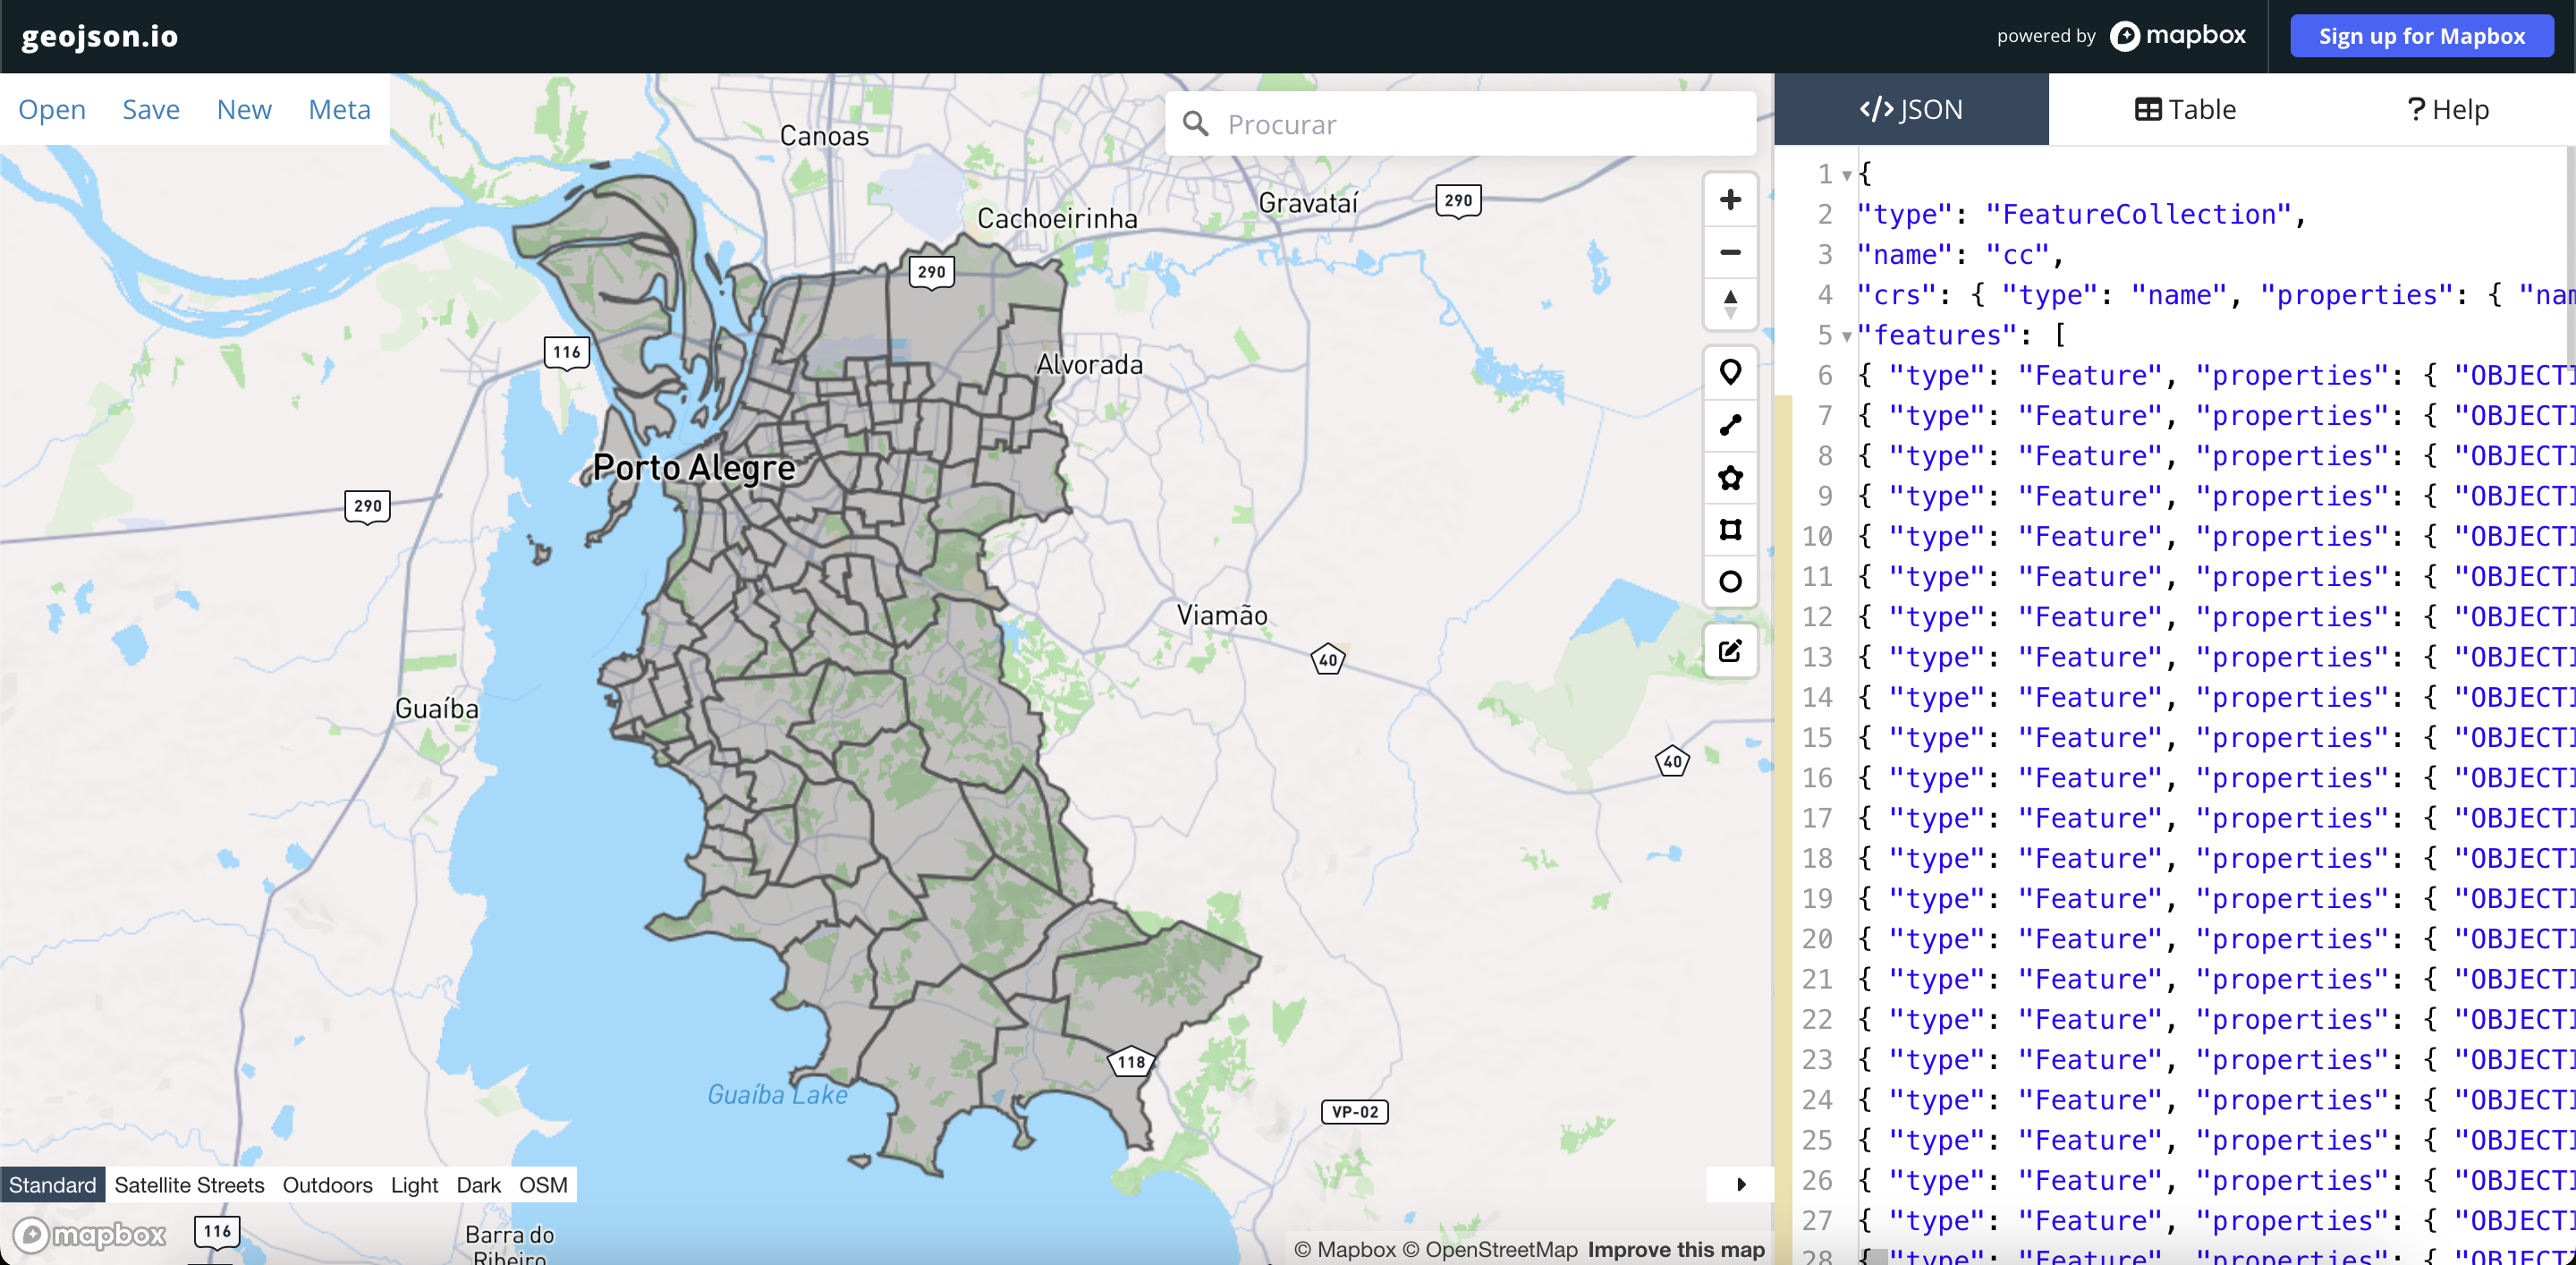
\includegraphics[width=\textwidth]{Capitulos/images/geojson.png}
    \caption{Visualização das coordenadas da cidade de Porto Alegre na aplicação GeoJson.io com os dados gerados na ferramenta QGIS.
    %GA: essa tela é só a visualização dos dados da prefeitura que tem os contorno dos bairros, certo? se não tem resultados da simulação nem criação desses dados, ajustar a legenda (GV: corrigido)
    }
    \label{fig:geojson}
\end{figure}

A apresentação dos resultados obtidos na simulação faz parte da mesma aplicação de interface gráfica utilizada na geração dos parâmetros do modelo de simulação. A tela inicial da apresentação dos resultados (Figura~\ref{fig:result_simulacao_1}) permite que o usuário interaja com duas ações: escolhendo o dia e hora (passo) da simulação para visualizar os resultados (Figura~\ref{fig:result_simulacao_1}(a)) e selecionando um bairro no mapa para obter informações detalhadas sobre os hospitais daquele bairro no passo de simulação selecionado (Figura~\ref{fig:result_simulacao_1}(b)). As cores no mapa representam a lotação geral dos hospitais naquele bairro, onde as cores de tom verde representam pouco uso dos leitos e as de tom vermelho representa superlotação dos leitos. No contexto da Figura~\ref{fig:result_simulacao_1} estão presentes hospitais em duas regiões simuladas, Teresópolis e Agronomia, no tempo de simulação do dia 0 e hora 0 eles apresentam um baixo uso dos leitos (tons verdes).

\begin{figure}
    \centering
    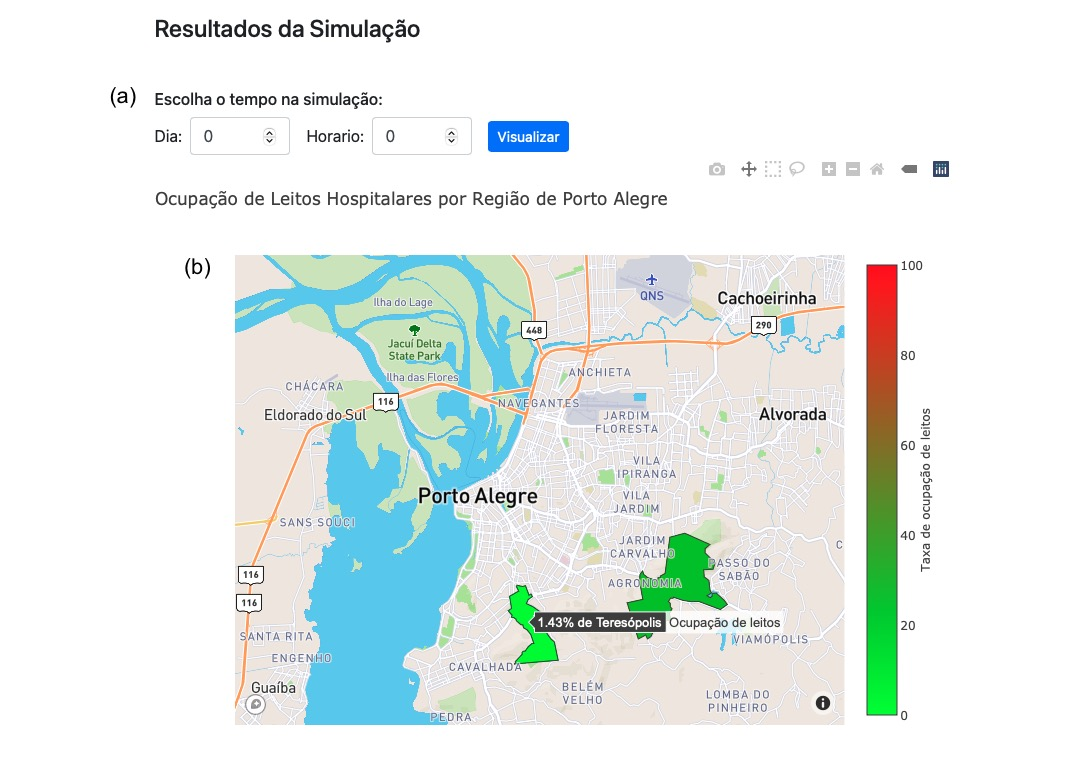
\includegraphics[width=\textwidth]{Capitulos/images/result1.jpeg}
    \caption{Tela inicial dos resultados da simulação.}
    \label{fig:result_simulacao_1}
\end{figure}

Ao selecionar um bairro no mapa, estão disponíveis informações relacionadas à lotação dos leitos hospitalares. A Figura~\ref{fig:result2} apresenta essas informações. Para cada hospital da região, estão disponíveis as seguintes informações: nome do hospital (Figura~\ref{fig:result2}(a)), porcentagem da ocupação total de leitos e dos leitos SUS (Figura~\ref{fig:result2}(b)), lista de ocupação das especialidades do hospital (Figura~\ref{fig:result2}(c)) e a opção de geração de texto para aquela especialidade (Figura~\ref{fig:result2}(d)). No exemplo, estão sendo apresentadas as informações do hospital HEPA do bairro Teresópolis, o hospital tem 1,43\% da ocupação total dos leitos utilizada e 2,3\% dos leitos SUS, abaixo apresenta os dados de cada especialidade de leito individualmente, para o leito ``Psquiatria'' do tipo ``Outras especialidades'' estão sendo utilizados 3 leitos, sendo os 3 leitos SUS e para a especialidade ``Saúde Mental'' do tipo ``Hospital Dia'' está sendo utilizado 1 leito e também sendo um leito SUS. A seção a seguir vai apresentar o processo de geração de texto médico (Figura~\ref{fig:result2}(d)) como exemplo para uma determinada especialidade.

%GA: acho que aqui cabe uma colinha melhor com a proxima section, ja que ela é um pouco diferente do resto (GV: corrigido)

\begin{figure}
    \centering
    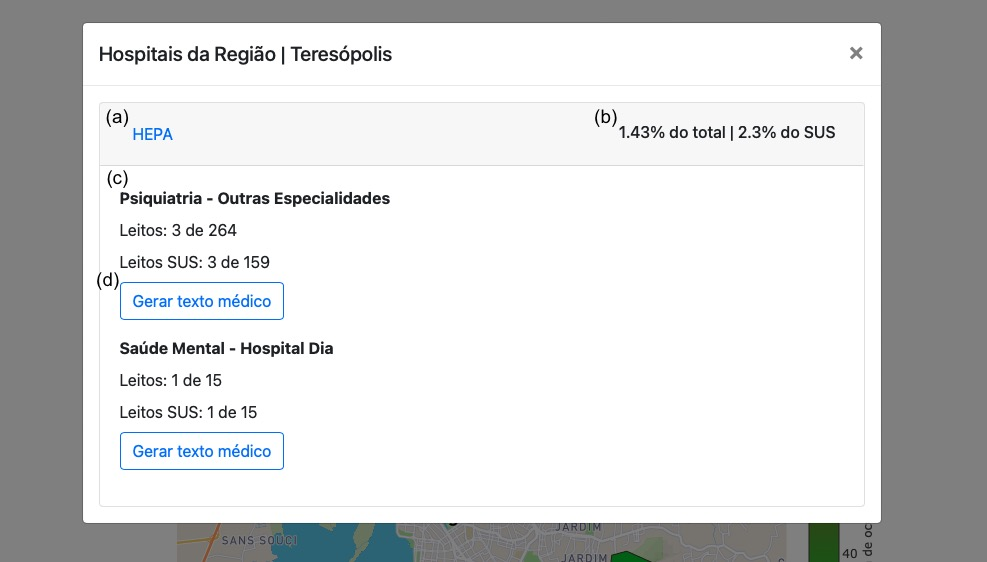
\includegraphics[width=\textwidth]{Capitulos/images/result2.jpeg}
    \caption{Resultados de um passo simulação em um bairro selecionado.}
    \label{fig:result2}
\end{figure}


\section{Geração de Texto Médico Individualizado}\label{sec:geracao_texto}
Para a geração de texto médico (Figura~\ref{fig:result2}(d)), utilizou-se da OpenAI API, apresentada na Seção~\ref{sec:chat}. Ao clicar no botão ``Gerar texto médico'', dispara-se um evento de comunicação com a API utilizando a seguinte estrutura de \textit{prompt}, definida com o auxílio de profissionais da área da medicina:

%GA: colocar o texto abaixo em um verbatim ou alguma extrutura diferenciada, esta mt similar ao texto mas não pertence diretamente a ele
\begin{spverbatim}
Imagine que você é um médico trabalhando no hospital na emergência. Você é 
responsável por atender os pacientes que chegam via emergência para 
especialidade ``(ESPECIALIDADE)'' do tipo ``(TIPO DE ESPECIALIDADE)'' para 
internação em um leito (SUS), que apresentam  diferentes apresentações 
e diagnósticos, desde quadros leves quanto quadros graves. Você faz a primeira 
avaliação médica, que abrange a anamnese e o exame físico. Após avaliar 
o paciente você decide as condutas que devem ser tomadas para internação do 
paciente, quais os próximos passos a serem feitos. Você precisa registrar essa 
avaliação médica no prontuário do paciente, ou seja, você precisa evoluir o 
paciente no sistema. Essa evolução deve ser sucinta, usando siglas médicas 
quando adequado e deve incluir os seguintes tópicos:

Nome do setor que você está atendendo em MAIÚSCULO.
O identificador do paciente deve ser: (IDENTIFICADOR)
Lista de problemas do paciente. Aqui você deve citar:
Os problemas de saúde prévios do paciente.
Medicações em uso de o paciente fizer uso de algum medicamento de uso contínuo
Uso de drogas: escrever se paciente fuma, bebe usa outras drogas ou não. Pode 
descrever a carga tabágica em maços/ano do paciente se ele for fumante.
HDA: História da doença atual
Aqui você deve escrever de forma sucinta o motivo que fez o paciente procurar 
atendimento médico.
Subjetivo: Aqui você deve escrever as informações relatadas pelo paciente ou 
familiar que sejam relevantes sobre a história do adoecimento. Como por 
exemplo, quando o quadro começou, quais os sintomas e sinais associados, como 
evoluiu até a procura do atendimento médico e etc.
Objetivo: Aqui você deve escrever o exame físico do paciente de forma sucinta 
e composto no mínimo por: Estado geral do paciente, avaliação do sensório, ausculta cardíaca, ausculta pulmonar, abdômen, extremidades.
Pode conter também outras informações conforme sejam necessárias a avaliação 
clinica conforme o quadro do paciente, como avaliação de deficit de força no 
avc, pele em afecções dermatológicas, etc. Você como médico deve buscar no 
exame físico do paciente achados que sejam relevantes para o quadro do 
paciente.
Logo abaixo do objetivo ou antes, você pode descrever resultados de exames 
laboratoriais e/ou de imagem do paciente que tenham sido realizados para 
avaliação do quadro dele. Anote sempre o nome do exame e a data da realização 
dele.
Impressão: Aqui você deve escrever as suas impressões gerais do quadro do 
paciente, como diagnósticos possíveis, gravidade
Conduta: aqui você deve listar as suas ações tomadas como médico, ou seja, as 
condutas que você tomou. Por exemplo: medicamentos prescritos ou removidos, 
solicitação de exames, consultoria com especialistas, descrição sucinta de 
conversas com familiares ou outros membros da equipe assistencial, Orientações 
para a alta se houverem, encaminhamentos, transferências.
\end{spverbatim}
%SO: achei que o texto acima poderia estar dentro de um quadro, outra fonte... sei lá... (GV: corrigido)

%SO: abaico tem figura para ilustrar essa parte?
Pela utilização da interface gráfica, o usuário pode definir o contexto do texto a ser gerado, ou seja, dentre as opções de leitos configuradas, o usuário seleciona qual especialidade e tipo de leito deseja retornar gerar exemplos de texto de evolução de pacientes (Figura~\ref{fig:result2}). Ao selecionar, é sorteado algum dos pacientes que estão internados no hospital naquela especialidade de leito e os campos (ESPECIALIDADE), (TIPO DE ESPECIALIDADE), (SUS) e (IDENTIFICADOR) do texto acima são substituídos pelas informações do paciente no contexto selecionado, a seguir é enviado como \textit{prompt} para a API. Abaixo se tem um exemplo de uma geração de texto para a especialidade ``Psiquiatria'' do tipo de leito ``Outras Especialidades'' atribuído a um leito privado.

\begin{spverbatim}
SETOR DE EMERGÊNCIA PSIQUIÁTRICA

IDENTIFICADOR DO PACIENTE: b4555eab-2565-4a22-ac22-028fe7bb9f38

Lista de Problemas:
- Saúde Prévia: Diabetes tipo 2 em tratamento com metformina.
- Medicações em Uso: Metformina 850mg, 1 comprimido duas vezes ao dia.
- Uso de Drogas: Nega tabagismo, consumo moderado de álcool socialmente.

HDA (História da Doença Atual):
Paciente apresenta quadro de agitação psicomotora e alucinações auditivas há 2 dias.

Subjetivo:
Relatado pela paciente: Início gradual dos sintomas, piora progressiva da agitação e desconforto psíquico associado às vozes que ouve.

Objetivo:
- Estado Geral: Paciente agitada, inquieta, olhar ansioso.
- Avaliação do Sensório: Desorientada no tempo, alerta quanto a pessoa e lugar.
- Ausculta Cardíaca: Ritmo cardíaco regular, sem sopros.
- Ausculta Pulmonar: Murmúrios vesiculares presentes bilateralmente.
- Abdômen: Macio, indolor à palpação, sem visceromegalias.
- Extremidades: Sem edemas ou sinais de trombose venosa profunda.

Resultados de Exames:
- Eletrocardiograma (ECG) realizado em 05/04/2024: Sem alterações significativas.

Impressão:
Possível episódio de psicose aguda em contexto de diabetes descompensada.

Conduta:
1. Prescrição de haloperidol 5mg via intramuscular para controle da agitação.
2. Solicitação de glicemia capilar para avaliação da glicemia atual.
3. Comunicação com a equipe de endocrinologia para avaliação e ajuste do tratamento antidiabético.
4. Orientação para acompanhamento psiquiátrico após a estabilização do quadro agudo.
5. Discussão do caso com equipe multidisciplinar para monitoramento contínuo da paciente.

Registro realizado em 05/04/2024.
\end{spverbatim}

Nos próximos capítulos serão analisados e discutidos os resultados de diferentes contextos de simulação utilizando o modelo apresentado nesse capitulo.

%SO: Faltou explicar como selecionaste o indivídulo. Da fig 4.15, tem vários leit0s.... de quem geraste? todos? como selecionas? (GV: revisao)

%SO: ainda aqui, é legal mostrar um exemplod e geração, não terminar tão bruscamente o capítulo. E indicar, ao final do capítulo, que no próximo serão analisados e discutidos os resutlados... (GV: corrigido)

%GA: se tu conseguir montar um video curto (captura de tela mesmo) do processo de montagem da simulação, executar e ver os resultados, isso pode virar um footnote no final desse capitulo
\chapter{Resultados Experimentais} \label{cpt:result}
Neste capítulo, são apresentados os resultados obtidos pelo modelo de simulação em diferentes contextos. Serão comparados os resultados de três simulações em configurações de ambientes distintos, porém com o mesmo tempo total de simulação, i.e., o mesmo número de passos de simulação, totalizando 12 passos, configurados em um período de 3 dias, com duração de 4 horas cada. Por fim, é feita uma demonstração dos resultados do modelo de geração de textos médicos a partir da API da OpenAI.

\section{Simulação 1}\label{sec:simul1}
Para a primeira simulação, considerou-se uma configuração do ambiente com apenas um hospital e com uma chegada de pacientes moderada considerando a capacidade total dos leitos. Foi escolhido o hospital HEPA, localizado no bairro Teresópolis e com as seguintes configurações de leitos:

\begin{itemize}
    \item ``Psquiatria'' do tipo ``Outras Especialidades'' contendo um total de 264 leitos, sendo 159 leitos SUS;
    \item ``Saúde Mental'' do tipo ``Hospital Dia'' contendo um total de 15 leitos, sendo os 15 leitos SUS.
\end{itemize}

Para fins de teste do modelo de simulação, para a especialidade ``Psiquiatria'', foi considerado um total de 500 internações durante o período de simulação, das quais 300 das internações são alocadas em leitos do SUS. Também foi informado que cada paciente ocupará, em média, de 1 a 4 passos de simulação enquanto estiver no leito hospitalar. Na especialidade ``Saúde Mental'', considera-se a ocorrência de 50 internações, das quais todas as 50 são em leitos do SUS. Nessa especialidade, os pacientes também permanecerão internados por um intervalo de 1 a 4 passos de simulação. A Figura~\ref{fig:simul-config-1} apresenta um recorte da configuração do ambiente na interface gráfica.

\begin{figure}
    \centering
    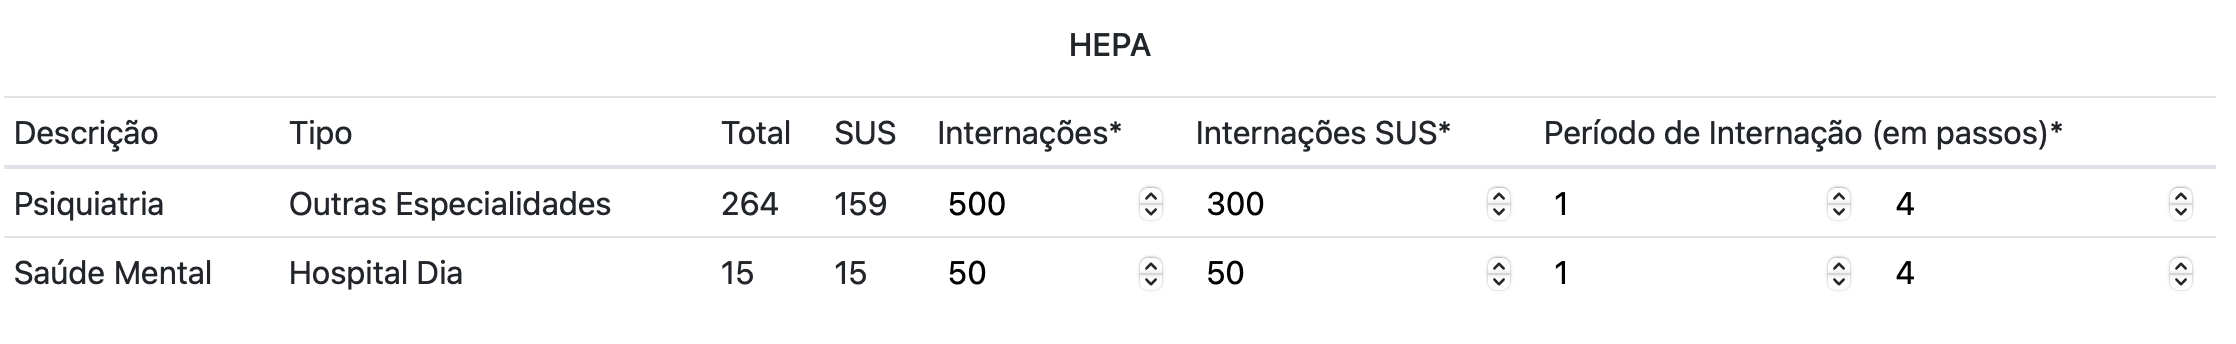
\includegraphics[width=\textwidth]{Capitulos/images/simul-config-1.png}
    \caption{Configuração dos leitos do hospital HEPA na simulação.}
    \label{fig:simul-config-1}
\end{figure}

Após a execução da simulação no contexto apresentado anteriormente, o resultado demonstrou que durante o período informado, e com os parâmetros selecionados, o leito da especialidade ``Psiquiatria'' não chegou a sua lotação máxima. No entanto, o leito da especialidade ``Saúde Mental'' passou da capacidade total de leitos no décimo primeiro passo de simulação, caracterizando uma superlotação no setor, isso se deu devido ao fluxo de entrada e saída dos pacientes nos leitos do hospital. As Figuras~\ref{fig:simulacao1-ocupacao1} e \ref{fig:simulacao1-ocupacao2} mostram o estado dos leitos em cada um dos passos de execução da simulação. As linhas em azuis nos gráficos representam a quantidade de leitos sendo utilizados no passo de simulação e as linhas em amarelo a capacidade de leitos daquela especialidade no hospital.

%GA: a tabela abaixo poderia ser um grafico de linhas, com uma linha para cada hospital (e pontilhada para SUS, por exemplo). (GV: corrigido)
%GA: também poderia ter o plot do limite de leitos como uma linha na horizontal (GV: corrigido)
%GA: acho que ficou melhor como grafico de linhas do que a tabela. Talvez não seja um problema os eixos Y n serem alinhados por não ser a mesma disponibilidade de leitos, mas é uma boa confirmar com a Soraia

\begin{figure}
\centering
\begin{subfigure}{0.49\textwidth}
    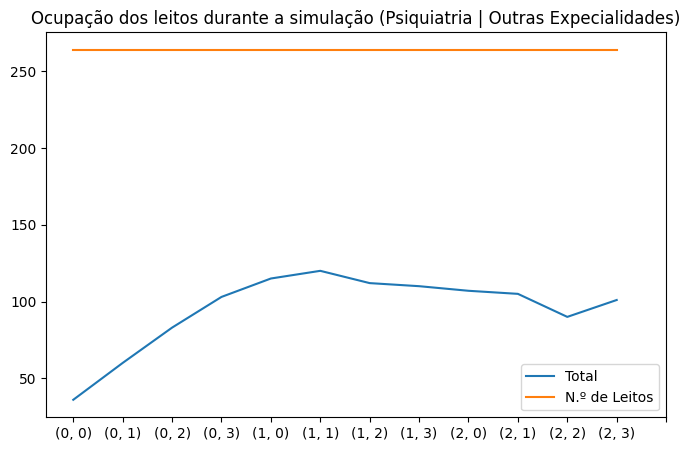
\includegraphics[width=\textwidth]{Capitulos/images/simul-psi-1.png}
    \caption{Ocupação dos leitos.}
\end{subfigure}
\hfill
\begin{subfigure}{0.5\textwidth}
    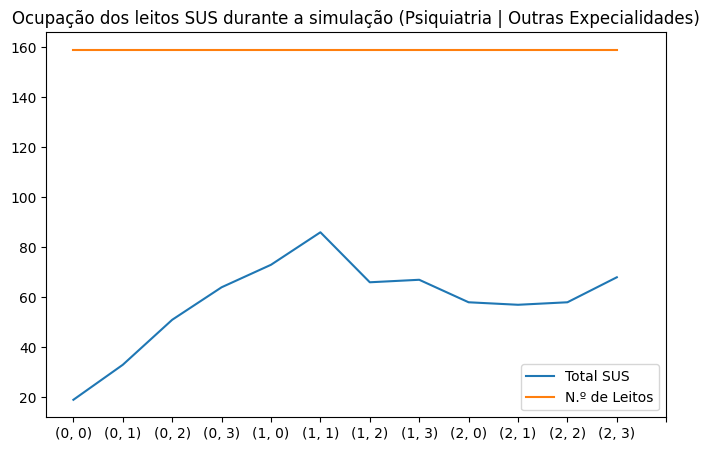
\includegraphics[width=\textwidth]{Capitulos/images/simul-psi-2.png}
    \caption{Ocupação dos leitos SUS.}
\end{subfigure}
        
\caption{Ocupação dos leitos durantes os passos de simulação para a especialidade ``Psquiatria'' do tipo ``Outras Especialidades'' do hospital HEPA.}
\label{fig:simulacao1-ocupacao1}
\end{figure}

\begin{figure}
    \centering
    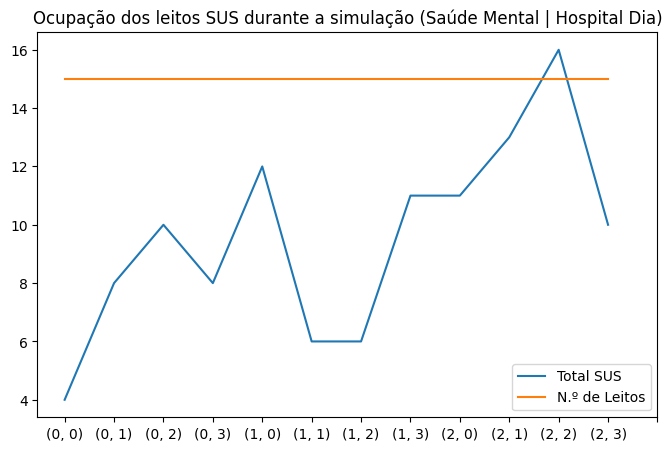
\includegraphics[width=0.5\textwidth]{Capitulos/images/simul-mental.png}
    \caption{Ocupação dos leitos SUS durantes os passos de simulação para a especialidade ``Saúde mental'' do tipo ``Hospital Dia'' do hospital HEPA.}
    \label{fig:simulacao1-ocupacao2}
\end{figure}

% \begin{table}[h!]
% \centering
% \begin{tabular}{ |l|l|l|l| } 
%  \hline
%  Passo & Leito & Total & Total SUS \\ 
%  \hline
%  1 & Psiquiatria - Outras Especialidades & 36 & 19\\  \hline
%  1 & Saúde Mental - Hospital Dia & 4 & 4\\  \hline
%  2 & Psiquiatria - Outras Especialidades & 60 & 33\\  \hline
%  2 & Saúde Mental - Hospital Dia & 8 & 8\\  \hline
%  3 & Psiquiatria - Outras Especialidades & 83 & 51\\  \hline
%  3 & Saúde Mental - Hospital Dia & 10 & 10\\  \hline
%  4 & Psiquiatria - Outras Especialidades & 103 & 64\\  \hline
%  4 & Saúde Mental - Hospital Dia & 8 & 8\\  \hline
%  5 & Psiquiatria - Outras Especialidades & 115 & 73\\  \hline
%  5 & Saúde Mental - Hospital Dia & 12 & 12\\  \hline
%  6 & Psiquiatria - Outras Especialidades & 120 & 86\\  \hline
%  6 & Saúde Mental - Hospital Dia & 6 & 6\\  \hline
%  7 & Psiquiatria - Outras Especialidades & 112 & 66\\  \hline
%  7 & Saúde Mental - Hospital Dia & 6 & 6\\  \hline
%  8 & Psiquiatria - Outras Especialidades & 110 & 67\\  \hline
%  8 & Saúde Mental - Hospital Dia & 11 & 11\\  \hline
%  9 & Psiquiatria - Outras Especialidades &107 & 58\\  \hline
%  9 & Saúde Mental - Hospital Dia & 11 & 11\\  \hline
%  10 & Psiquiatria - Outras Especialidades & 105 & 57\\  \hline
%  10 & Saúde Mental - Hospital Dia & 13 & 13\\  \hline
%  11 & Psiquiatria - Outras Especialidades & 90 & 58\\  \hline
%  11 & Saúde Mental - Hospital Dia & 16 & 16\\  \hline
%  12 & Psiquiatria - Outras Especialidades & 101 & 68\\  \hline
%  12 & Saúde Mental - Hospital Dia & 10 & 10\\  \hline
% \end{tabular}
% \caption{Estados dos leitos hospitalares para cada passo de simulação.}
% \label{table:result1}
% \end{table}

A Figura~\ref{fig:simul-result-1} ilustra alguns dos estados da ocupação dos leitos do hospital HEPA na interface gráfica. A Figura~\ref{fig:simul-result-1}(a) apresenta o estado do hospital após o final da execução do primeiro passo de simulação, com 14.34\% do total de leitos hospitalares ocupados, e a Figura~\ref{fig:simul-result-1}(b) demonstra esses dados após o final da execução do ultimo passo de simulação, com 39.78\% do total dos leitos hospitalares ocupados.

\begin{figure}
\centering
\begin{subfigure}{0.8\textwidth}
    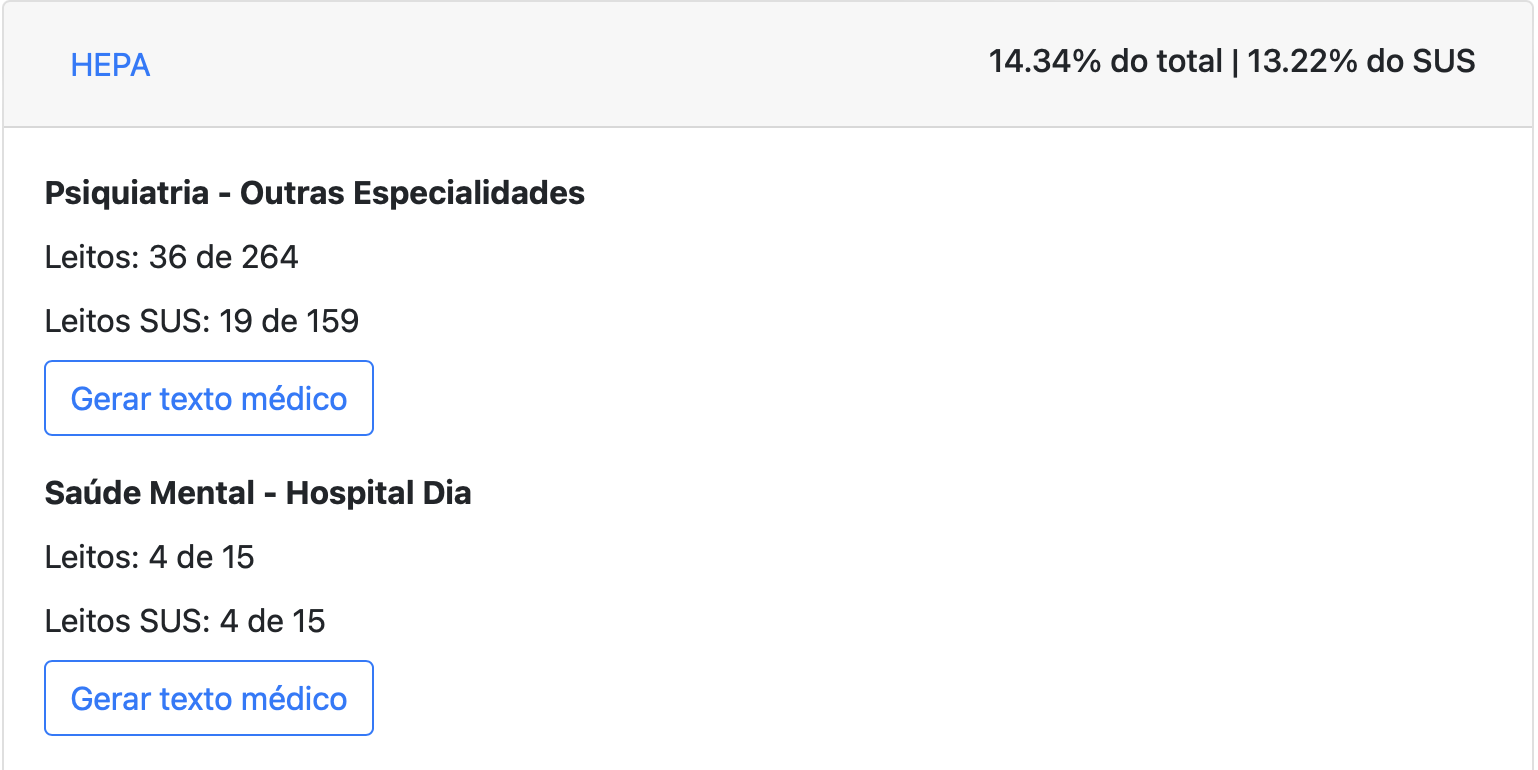
\includegraphics[width=\textwidth]{Capitulos/images/simul-result-1a.png}
    \caption{Estado dos leitos do hospital HEPA ao final do primeiro passo de simulação.}
    \label{fig:first}
\end{subfigure}
\hfill
\begin{subfigure}{0.8\textwidth}
    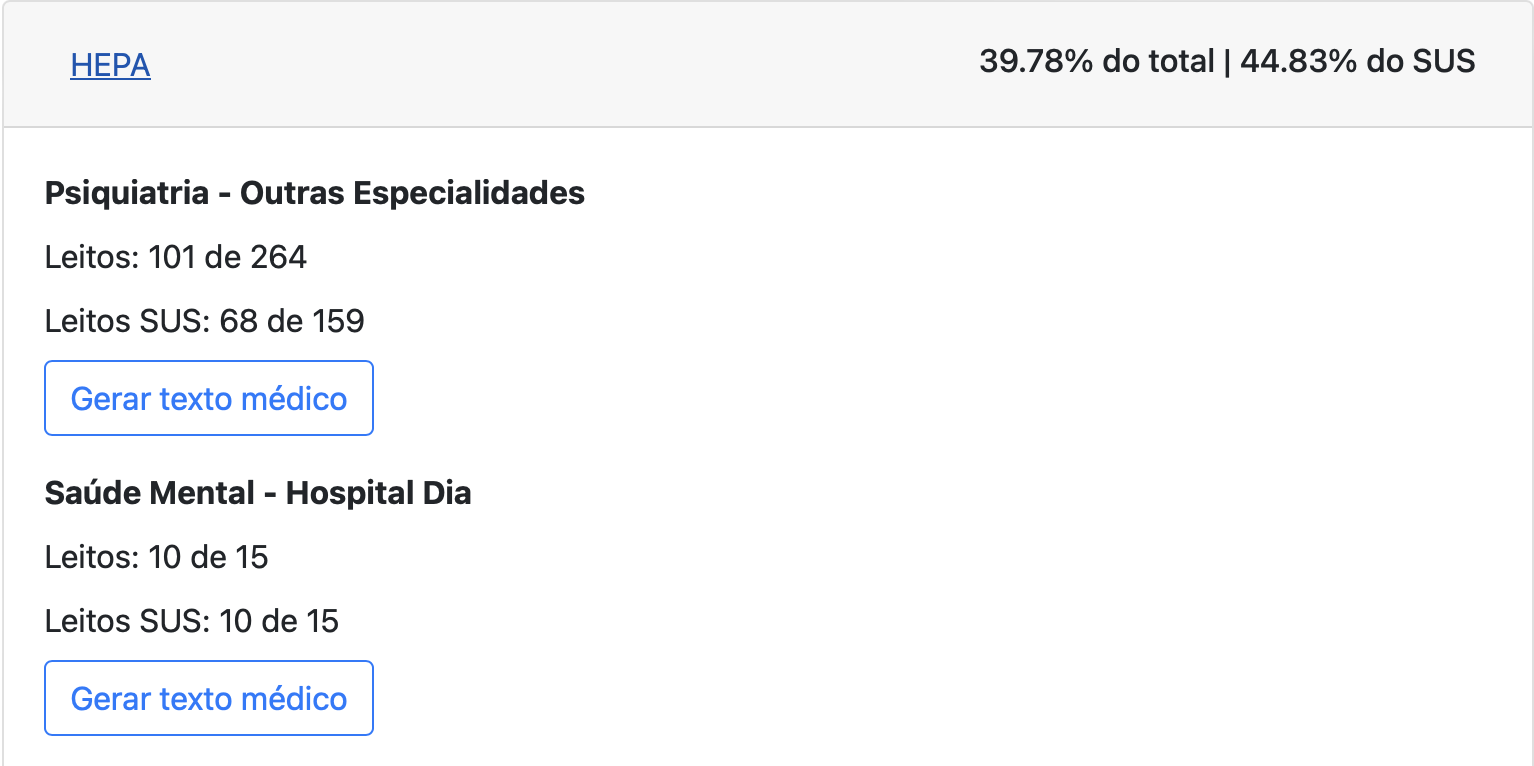
\includegraphics[width=\textwidth]{Capitulos/images/simul-result-1b.png}
    \caption{Estado dos leitos do hospital HEPA ao final do ultimo passo de simulação.}
    \label{fig:second}
\end{subfigure}
        
\caption{Resultados no primeiro e ultimo passo de simulação.}
\label{fig:simul-result-1}
\end{figure}

% \subsection{Geração de texto}
% Conforme apresentado na Seção~\ref{sec:geracao_texto}, para geração do texto médico é selecionado um paciente aleatório dentre os internados em uma especialidade de leito hospitalar especifica. O leito selecionado para geração do texto foi o de especialidade ``Saúde Mental'' do tipo de leito ``Hospital Dia''. A seguir é apresentado o texto gerado pela API da OpenAI e a descrição das características do paciente selecionado na Listagem~\ref{lst:select_paciente}. 

% \begin{spverbatim} 
% Lista de Problemas:

% Saúde Prévia: Não há histórico de doenças crônicas conhecidas.
% Medicações em Uso: Nenhuma medicação de uso contínuo registrada.
% Uso de Drogas: Nega tabagismo, consumo ocasional de álcool.
% HDA (História da Doença Atual):
% Paciente procurou atendimento devido a sintomas de ansiedade e depressão, com piora progressiva nos últimos meses.

% Subjetivo:
% Relatado pela paciente: Início gradual dos sintomas, incluindo tristeza persistente, insônia, falta de interesse em atividades diárias e pensamentos suicidas recentes.

% Objetivo:

% Estado Geral: Paciente apresenta-se abatida, com expressão facial entristecida.
% Avaliação do Sensório: Orientada no tempo, espaço e pessoa, porém com humor deprimido.
% Ausculta Cardíaca: Ritmo regular, sem sopros.
% Ausculta Pulmonar: Murmúrios vesiculares presentes bilateralmente.
% Abdômen: Sem alterações significativas à palpação.
% Extremidades: Sem edema, pulsos palpáveis bilateralmente.
% Resultados de Exames:

% Hemograma completo realizado em 05/04/2024: Dentro dos limites da normalidade.
% Eletrocardiograma (ECG) realizado em 05/04/2024: Sem anormalidades significativas.
% Impressão:
% Quadro sugestivo de transtorno depressivo maior com sintomas ansiosos, de gravidade moderada.

% Conduta:

% Encaminhamento para avaliação psiquiátrica completa.
% Prescrição de sertralina 50mg ao dia para tratamento da depressão, com acompanhamento ambulatorial.
% Encaminhamento para psicoterapia regular.
% Orientação para manutenção do acompanhamento médico e psicoterapêutico.
% Contato com familiar para apoio e monitoramento domiciliar.
% Registro realizado em 05/04/2024.
% \end{spverbatim}

% O texto gerado é coerente com a descrição da atividade solicitada ao modelo de geração de texto. No entanto, a informação sobre o tipo de leito associado ao paciente, seja privado ou SUS, não parece influenciar na geração do texto.

% \begin{listing}
% \begin{minted}[frame=single,
%                framesep=3mm,
%                linenos=true,
%                xleftmargin=21pt,
%                tabsize=4]{js}     
% {
%     'patient_id': 'b4ed248d-aaae-4d10-aad2-1f075a6a3003', 
%     'from_region': 'Teresópolis', 
%     'specialty': 'Saúde Mental', 
%     'type': 'Hospital Dia', 
%     'admission_time': 3, 
%     'return_frame': 3, 
%     'is_sus': True
% }
% \end{minted}
% \caption{Características do paciente na selecionado.} 
% \label{lst:select_paciente}
% \end{listing}

\section{Simulação 2}
A segunda simulação foi parametrizada com o mesmo hospital e especialidades de leitos hospitalares da simulação anterior, diferencia-se pela configuração da quantidade de internações durante o período de simulação. Com o objetivo de analisar um cenário de superlotação dos leitos hospitalares, foi considerado que o total de pacientes que chegam ao hospital durante o período de simulação fosse 10 vezes
%SO: 100 vezes seria 264*100 ou seja 26400...
a quantidade da capacidade dos leitos. Por exemplo, para o leito da especialidade ``Psiquiatria'' do tipo ``Outras Especialidades'' do hospital HEPA, estão disponíveis 264 espaços ao total, logo, na simulação serão encaminhados 2640 pacientes ao total para internação durante os 12 passos de simulação definido. A Figure~\ref{fig:simulacao2-a} ilustra a configuração do número de internações de pacientes na interface gráfica.

\begin{figure}
    \centering
    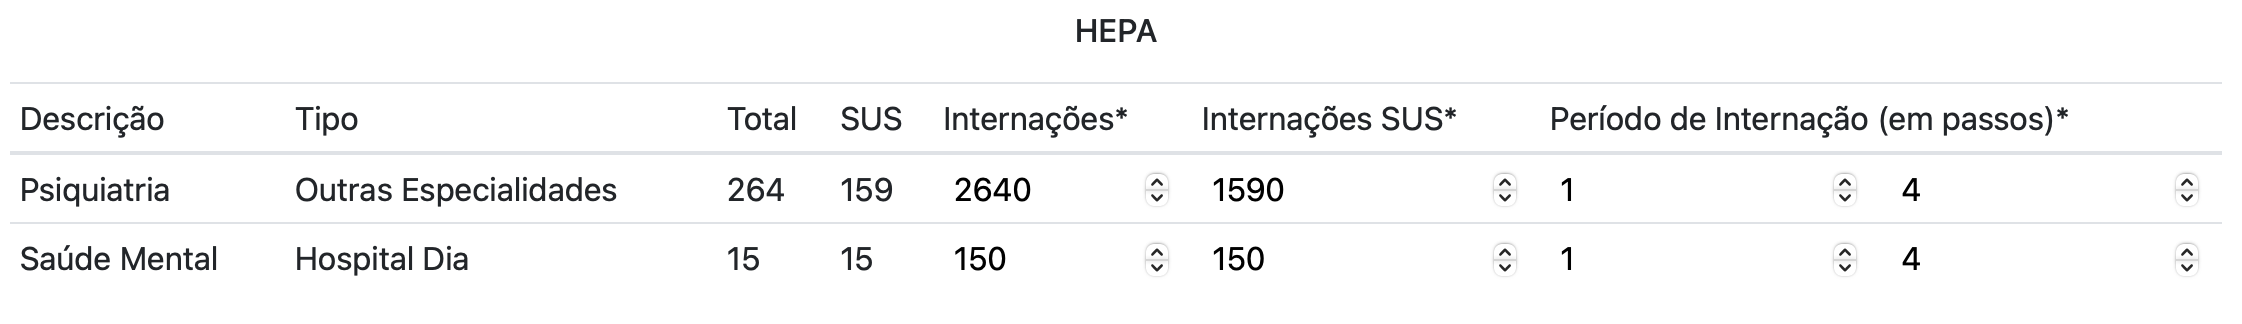
\includegraphics[width=\textwidth]{Capitulos/images/simulacao2-a.png}
    \caption{Configuração dos leitos do hospital HEPA na simulação.}%SO: falta caption na figura
    \label{fig:simulacao2-a}
\end{figure}

Realizada a simulação, pode-se observar que nos gráficos da Figura~\ref{fig:simulacao2} que dada a configuração utilizada, logo nos primeiros passos de simulação os leitos da especialidade ``Psiquiatria'' sofreram uma superlotação em ambos os tipos de leitos, privados e SUS. Já na Figura~\ref{fig:simulacao2b} os leitos da especialidade ``Saúde Mental'' superlotou no primeiro passo da simulação.

\begin{figure}
\centering
\begin{subfigure}{0.49\textwidth}
    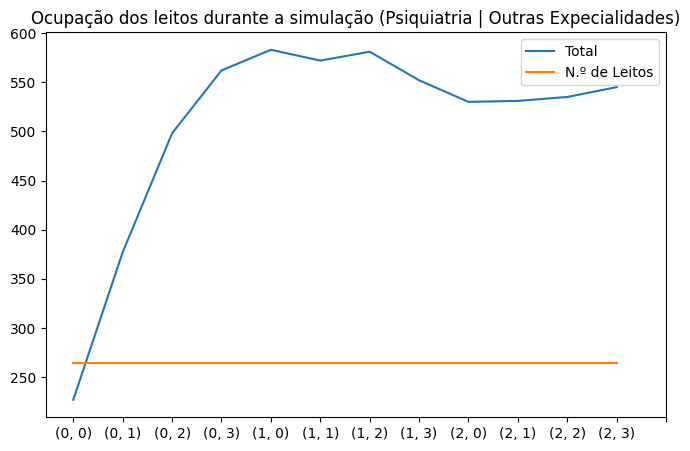
\includegraphics[width=\textwidth]{Capitulos/images/simulacao2-b.png}
    \caption{Ocupação dos leitos.}
    \label{fig:first}
\end{subfigure}
\hfill
\begin{subfigure}{0.49\textwidth}
    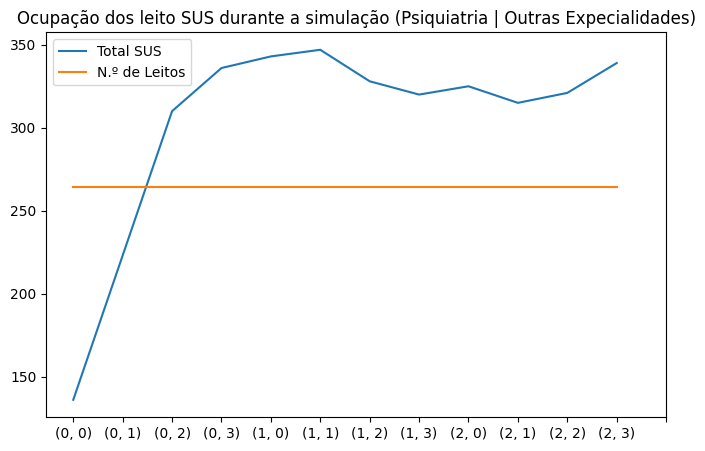
\includegraphics[width=\textwidth]{Capitulos/images/simulacao2-c.png}
    \caption{Ocupação dos leitos SUS.}
    \label{fig:second}
\end{subfigure}
        
\caption{Ocupação dos leitos durantes os passos de simulação para a especialidade ``Psquiatria'' do tipo ``Outras Especialidades'' do hospital HEPA.}
\label{fig:simulacao2}
\end{figure}

\begin{figure}
    \centering
    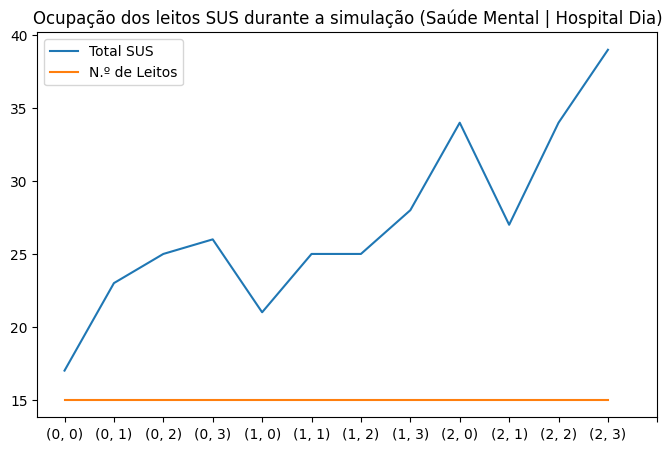
\includegraphics[width=0.5\textwidth]{Capitulos/images/simulacao2-d.png}
    \caption{Ocupação dos leitos SUS durantes os passos de simulação para a especialidade ``Saúde mental'' do tipo ``Hospital Dia'' do hospital HEPA.}
    \label{fig:simulacao2b}
\end{figure}

A Figura~\ref{fig:simulacao2-compare} apresenta uma comparação entre as diferentes simulações, apresentando o estado da ocupação dos leitos da região do hospital HEPA ao fim do primeira passo da simulação.

\begin{figure}
\centering
\begin{subfigure}{0.49\textwidth}
    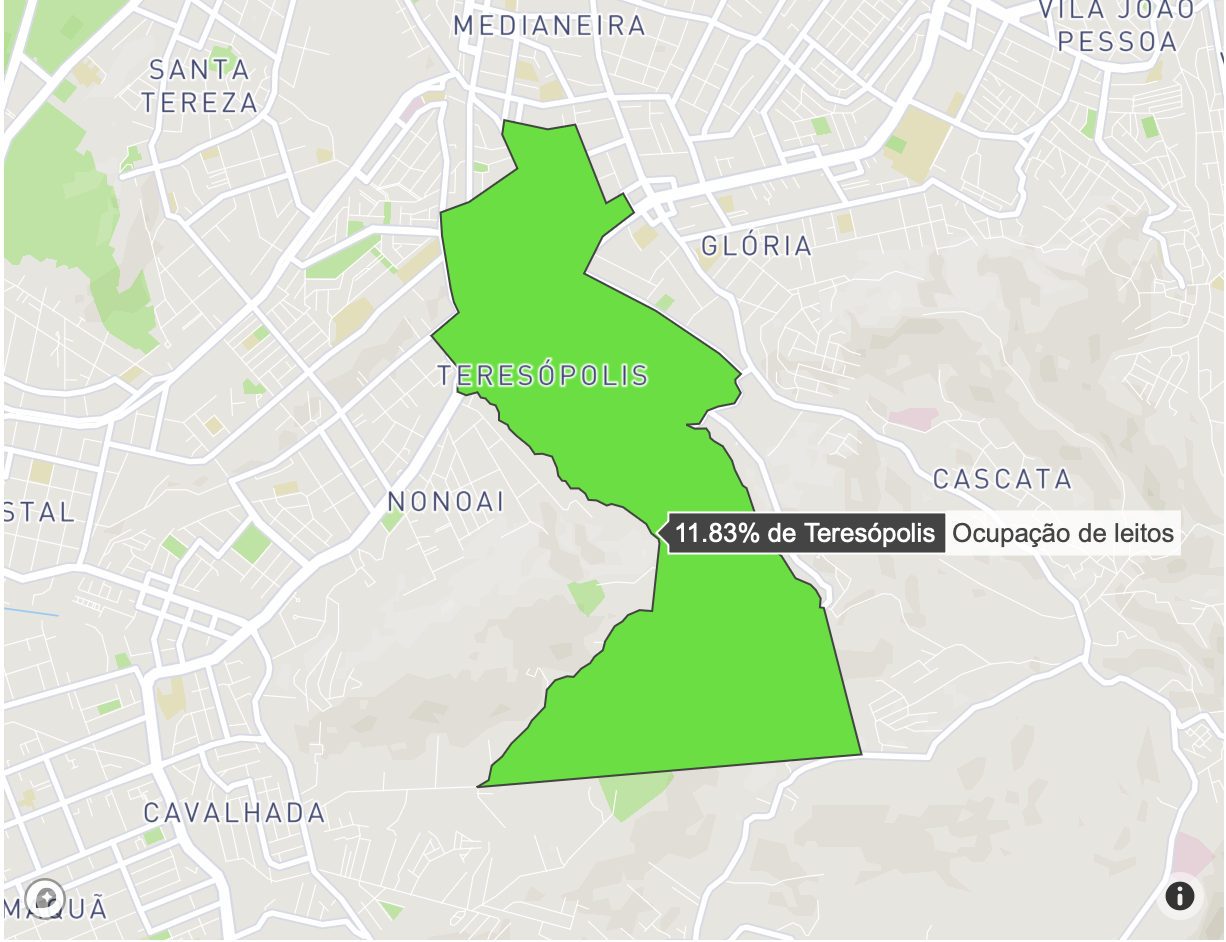
\includegraphics[width=\textwidth]{Capitulos/images/result2-compare-1.png}
    \caption{Ocupação dos leitos na simulação 1.}
    \label{fig:first}
\end{subfigure}
\hfill
\begin{subfigure}{0.49\textwidth}
    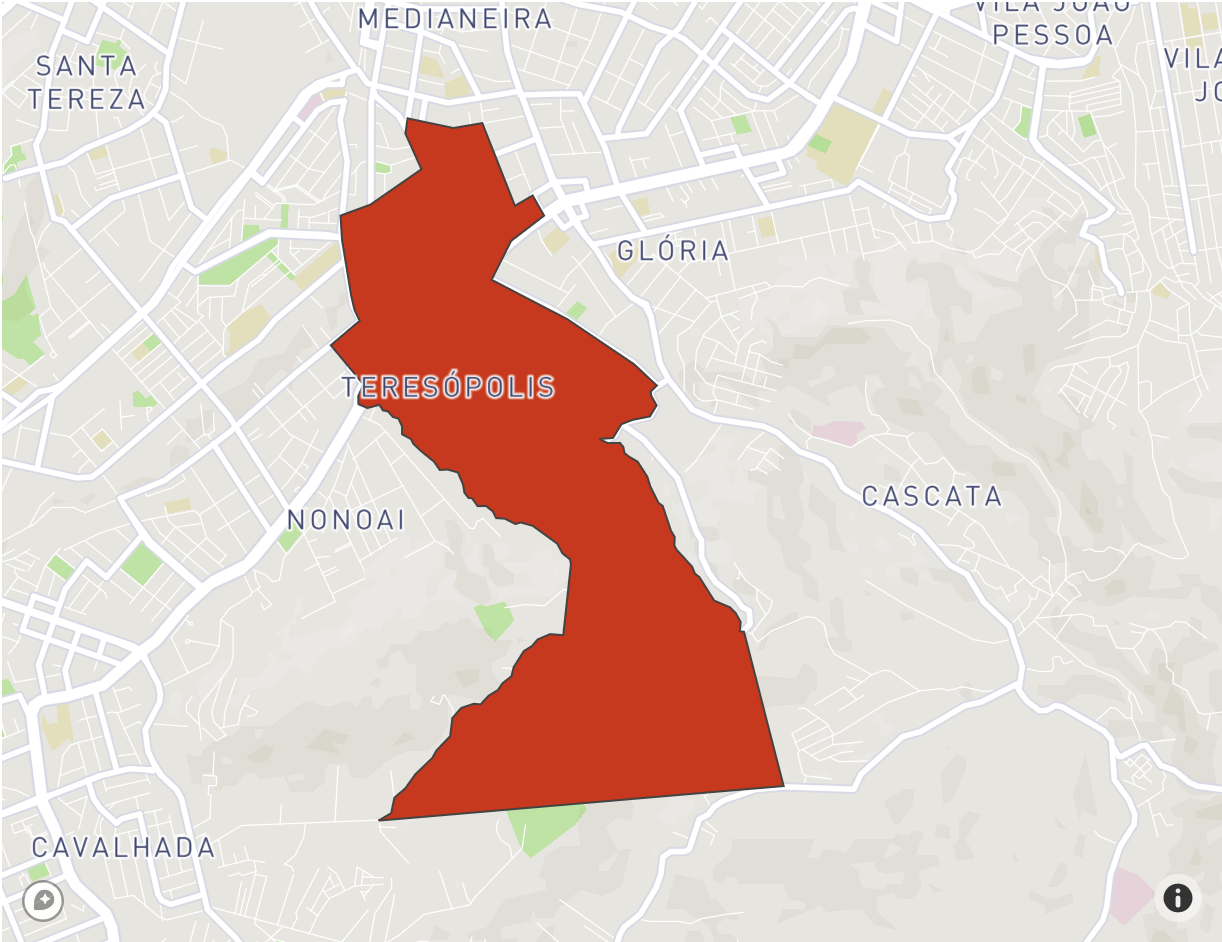
\includegraphics[width=\textwidth]{Capitulos/images/result2-compare-2.png}
    \caption{Ocupação dos leitos na simulação 2.}
    \label{fig:second}
\end{subfigure}
        
\caption{Comparação entre a ocupação dos leitos da região do hospital HEPA ao fim do primeiro passo de simulação nas simulações 1 e 2.}
\label{fig:simulacao2-compare}
\end{figure}

A simulação realizada indica que o modelo de simulação reproduz a superlotação dos conforme esperado, considerando a alta demanda de internações nos leitos hospitalares do HEPA configuradas pelo usuário na interface gráfica.

\section{Simulação 3}
A configuração utilizada na terceira simulação foi executada de forma a considerar dois hospitais no mesmo bairro, para isso, utilizamos os hospitais HEPA e Santa Ana, ambos localizados no bairro Teresópolis. Foi parametrizado que os hospitais teriam apenas uma especialidade de leito cada, a especialidade ``Psiquiatria'' do tipo ``Outras Especialidades''. Essa configuração foi criada com o objetivo de realizar uma comparação com o cenário da simulação anterior e entender o comportamento dos hospitais no caso de divisão dos pacientes entre eles. A Figura~\ref{fig:simulacao3a} ilustra a configuração dos dois hospitais na interface gráfica.

\begin{figure}
    \centering
    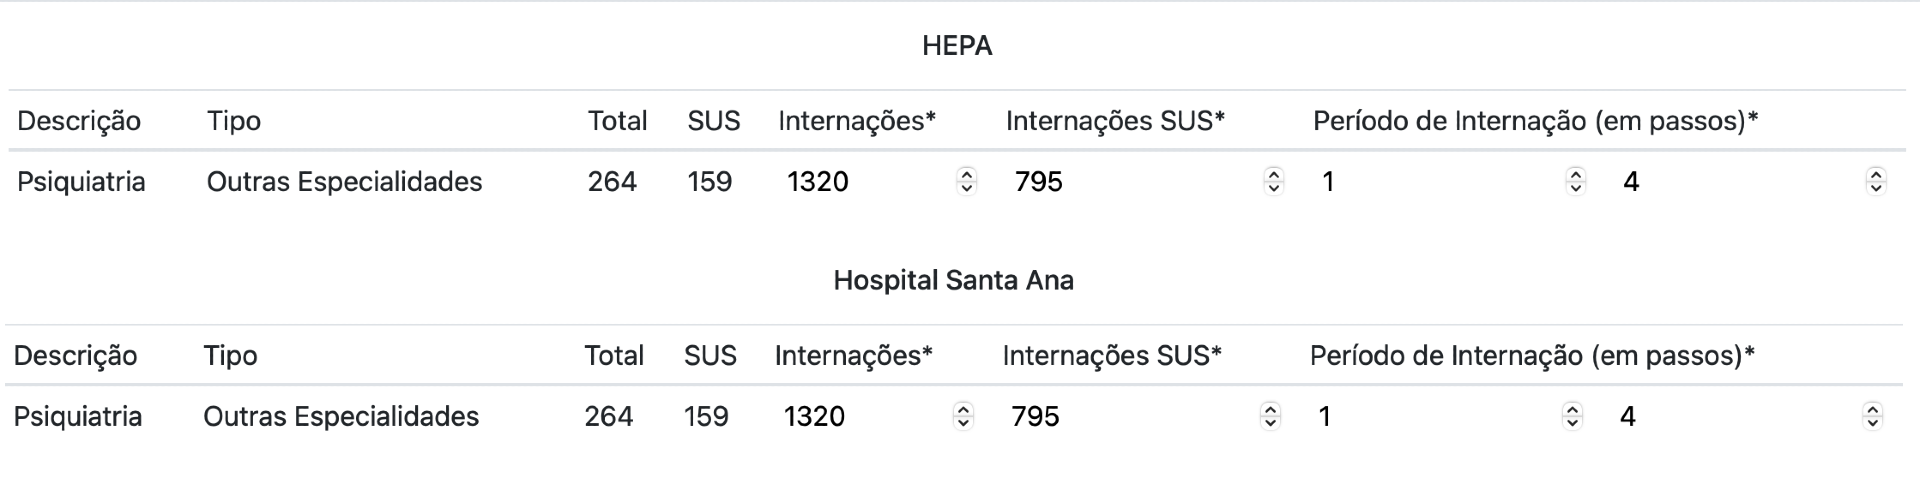
\includegraphics[width=\textwidth]{Capitulos/images/simulacao3-a.png}
    \caption{Configuração dos leitos dos hospitais HEPA e Santa Ana na simulação.}
    \label{fig:simulacao3a}
\end{figure}

A Figura~\ref{fig:simulacao3} apresenta os resultados dos passos de simulação para os dois hospitais considerando os leitos privados e SUS. Pode-se observar que a divisão dos pacientes entre os hospitais na simulação resulta em um tempo maior de execução até a superlotação do leito. Em comparação com a simulação anterior, o hospital HEPA (Figura~\ref{fig:simulacao3}(a)) que teve a superlotação dos leitos já no segundo passo de simulação, com a divisão entre os hospitais essa lotação dos leitos aconteceu apenas no passo 4 e voltou a ter leitos disponíveis no decimo primeiro passo, na simulação anterior os leitos permaneceram superlotados durante todos os passos de simulação seguintes. A Figura~\ref{fig:simulacao3}(b) ilustra o comportamento da ocupação dos leitos no hospital Santa Ana, onde observa-se um fluxo de ocupação semelhante ao do hospital HEPA e isso acontece devido aos dois hospitais possuírem as mesmas características em relação a essa especialidade de leito.

\begin{figure}
\centering
\begin{subfigure}{0.49\textwidth}
    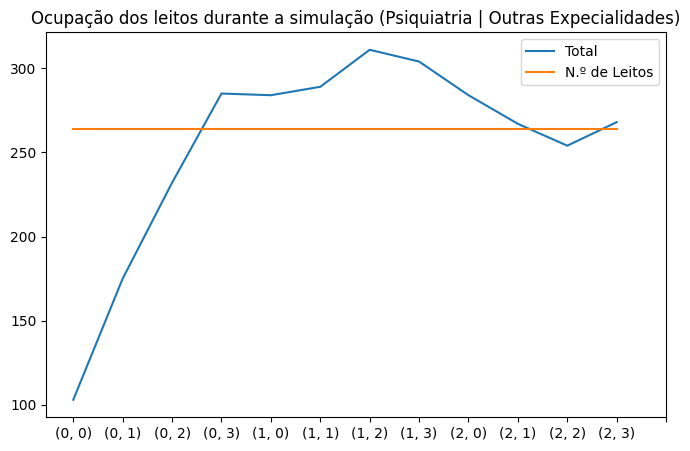
\includegraphics[width=\textwidth]{Capitulos/images/simulacao3-hepa.png}
    \caption{Ocupação dos leitos do hospital HEPA.}
    \label{fig:first}
\end{subfigure}
\hfill
\begin{subfigure}{0.49\textwidth}
    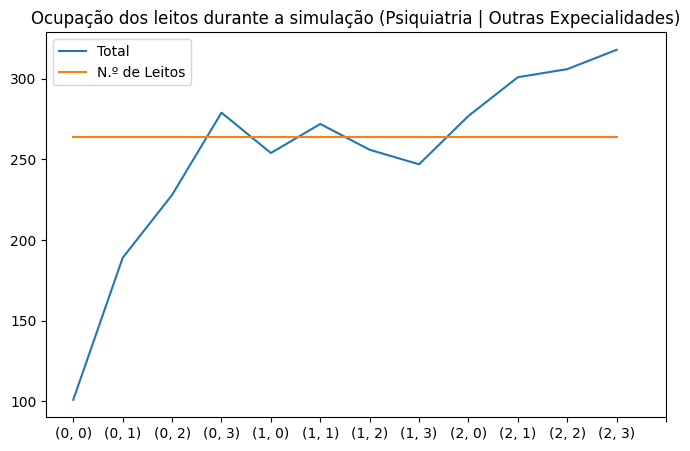
\includegraphics[width=\textwidth]{Capitulos/images/simulacao3-santaana.png}
    \caption{Ocupação dos leitos do hospital Santa Ana.}
    \label{fig:second}
\end{subfigure}
        
\caption{Ocupação dos leitos da especialidade “Psiquiatria” durante cada passo de simulação nos hospital HEPA e Santa Ana.}
\label{fig:simulacao3}
\end{figure}

Assim como no mundo real, inserir um novo hospital em uma região é uma possível abordagem para diminuir a ocupação dos leitos de um outro hospital próximo. Essa simulação demonstrou que o mesmo ocorre no ambiente de simulação ao disponibilizar um maior número de leitos para uma mesma demanda de internações apresentada na simulação anterior.

\section{Geração de Texto de Pacientes na Simulação}
Conforme apresentado na Seção~\ref{sec:geracao_texto}, para geração do texto médico é selecionado um paciente aleatório dentre os internados em uma especialidade de leito hospitalar especifica. Para a validação da geração de textos, foram selecionados pacientes internados nos leitos do hospital HEPA no sétimo passo da simulação da Seção~\ref{sec:simul1}. A Tabela~\ref{table:pacientes} mostra o percurso desses pacientes na simulação, sendo, a identificação do paciente (ID), a região de origem (Origem), a especialidade de leito em que foi internado (Leito), o passo de simulação em que chegou ao hospital (Chegada), em qual passo ele vai retornar para sua casa (Retorno) e se esta internado em um leito SUS ou privado (Setor).
 
\begin{table}[h!]
\centering
\begin{tabular}{ |l|l|l|l|l|l| } 
 \hline
 ID & Origem & Leito & Chegada & Retorno & Setor \\ 
 \hline
 f130ea18... & Teresópolis & Psiquiatria - Outras Especialidades & 4 & 8 & SUS \\ \hline
 3ee1981c... & Teresópolis & Psiquiatria - Outras Especialidades & 4 & 8 & SUS \\ \hline
 faab4cb8... & Teresópolis & Psiquiatria - Outras Especialidades & 4 & 8 & SUS \\ \hline
 b83792aa... & Azenha & Saúde Mental - Hospital Dia & 4 & 8 & SUS \\ \hline 
 f9d01e2f... & Santa Cecília & Saúde Mental - Hospital Dia & 4 & 9 & SUS  \\ \hline 
 85c85302... & Azenha & Saúde Mental - Hospital Dia & 3 & 8 & SUS \\ \hline
 \end{tabular}
\caption{Exemplos de pacientes internados no hospital HEPA no sétimo passo de simulação.}
\label{table:pacientes}
\end{table}

Para comparação da geração de texto médico em diferentes contextos utilizou-se de dois pacientes internados em especialidades de leitos distintos. Foram selecionados um paciente do leito de especialidade ``Psiquiatria'' do tipo ``Outras Especialidades'' e outro de ``Saúde Mental'' do tipo ``Hospital Dia''. A seguir é apresentado os textos médicos de evolução de pacientes gerados pelo modelo através da API da OpenAI. A geração do texto para o paciente internado em um leito de especialidade ``Psiquiatria'' do tipo ``Outras Especialidades'' retornou o seguinte resultado:

\begin{spverbatim}
SETOR DE EMERGÊNCIA PSIQUIÁTRICA

IDENTIFICADOR DO PACIENTE: f130ea18-5651-4eb7-b23b-ca8f2081d8ac

LISTA DE PROBLEMAS:
- Problemas de saúde prévios: Não há informações disponíveis sobre histórico 
médico prévio.
- Medicações em uso: Não há informações sobre uso prévio de medicamentos.
- Uso de drogas: Não há relato de uso de tabaco, álcool ou outras drogas.

HDA:
Paciente de 35 anos, sexo masculino, trazido pela família com queixa de 
agitação psicomotora, insônia e comportamento agressivo há 3 dias. Família 
relata que o paciente tem histórico de episódios similares, sem tratamento 
prévio.

SUBJETIVO:
Início súbito dos sintomas há 3 dias, segundo relato da família. 
Agressividade verbal e física, irritabilidade exacerbada, dificuldade para 
dormir, sem relato de alucinações ou delírios.

OBJETIVO:
- Estado geral: Paciente agitado, desorientado no tempo e no espaço.
- Sensório: Desorientado, reativo a estímulos verbais.
- Ausculta cardíaca: Ritmo cardíaco regular, sem sopros audíveis.
- Ausculta pulmonar: Murmúrio vesicular presente bilateralmente, sem ruídos 
adventícios.
- Abdômen: Sem alterações à palpação.
- Extremidades: Sem edema ou sinais de trauma.

EXAMES:
- Hemograma completo (05/04/2024): dentro dos valores de referência.
- Bioquímica sanguínea (05/04/2024): dentro dos valores de referência.

IMPRESSÃO:
Quadro compatível com episódio agudo de transtorno psicótico agudo, 
necessitando de avaliação psiquiátrica urgente.

CONDUTA:
1. Encaminhamento para avaliação psiquiátrica emergencial.
2. Sedação com benzodiazepínico conforme protocolo.
3. Manter em observação na emergência até avaliação psiquiátrica.
4. Orientações à família sobre a necessidade de acompanhamento psiquiátrico 
regular.
5. Solicitação de internação psiquiátrica compulsória, se necessário, de 
acordo com legislação vigente.
\end{spverbatim}

Após, o mesmo procedimento é aplicado para o paciente internado no leito de especialidade ``Saúde Mental'' do tipo ``Hospital Dia'' e o resultado do texto gerado foi o seguinte:

\begin{spverbatim}
SETOR DE SAÚDE MENTAL - HOSPITAL DIA

IDENTIFICADOR DO PACIENTE: f9d01e2f-de4e-430e-a663-b0454fda937d

LISTA DE PROBLEMAS:
- Problemas de saúde prévios: Transtorno de ansiedade generalizada.
- Medicações em uso: Sertralina 50mg/dia.
- Uso de drogas: Não há relato de tabagismo, consumo de álcool ou outras 
drogas.

HDA:
Paciente de 42 anos, sexo feminino, busca atendimento devido a piora dos 
sintomas de ansiedade e insônia nas últimas semanas, com dificuldade para 
realizar as atividades diárias.

SUBJETIVO:
Sintomas de ansiedade exacerbados nas últimas semanas, relatando preocupações 
excessivas, inquietação, dificuldade de concentração e irritabilidade. Refere 
insônia persistente, com dificuldade para iniciar e manter o sono.

OBJETIVO:
- Estado geral: Paciente aparenta ansiedade, porém coopera com o exame.
- Sensório: Alerta e orientada quanto ao tempo, espaço e pessoa.
- Ausculta cardíaca: Ritmo cardíaco regular, sem sopros audíveis.
- Ausculta pulmonar: Murmúrio vesicular presente bilateralmente, sem ruídos 
adventícios.
- Abdômen: Sem alterações à palpação.
- Extremidades: Sem edema ou sinais de trauma.

EXAMES:
- Hemograma completo (05/04/2024): dentro dos valores de referência.
- Bioquímica sanguínea (05/04/2024): dentro dos valores de referência.

IMPRESSÃO:
Transtorno de ansiedade generalizada, com piora dos sintomas interferindo 
nas atividades diárias.

CONDUTA:
1. Ajuste na dose de sertralina para 75mg/dia.
2. Encaminhamento para acompanhamento psicológico regular.
3. Orientações sobre técnicas de relaxamento e manejo do estresse.
4. Reavaliação em duas semanas para monitoramento da resposta ao tratamento.
\end{spverbatim}

Os textos gerados se demonstram coerentes com a descrição da atividade solicitada ao modelo de geração de texto. No entanto, a informação sobre o setor do leito associado ao paciente, seja privado ou SUS, não parece influenciar na geração do texto, já a especialidade, tipo de leito e o identificador do paciente são relevantes para o resultado do texto gerado. Os textos gerados estão associados a descrição de um único paciente para cada texto, assim, enfatizando a possibilidade de individualização da população do LODUS a partir do \textit{plugin} desenvolvido.
\chapter{Considerações Finais} \label{cpt:discus}
Este capítulo resume nossas contribuições para o desenvolvimento de pesquisa no uso de tecnologias para a área da saúde, as limitações da abordagem proposta e nossos planos futuros para continuidade da pesquisa.

\section{Contribuições}
Neste trabalho desenvolvemos um conjunto de dados com informações reais de quantidade de leitos hospitalares separados por especialidade e tipo nos hospitais de Porto Alegre, em complemento também adicionamos informações geográficas de latitude e longitude de cada hospital. Os dados coletados foram provenientes do Cadastro Nacional de Estabelecimentos de Saúde (CNES) disponibilizado pelo DATASUS e as informações geográficas coletadas no Google Maps. O conjunto de dados gerado pode ser utilizado em outras aplicações voltadas para a área da saúde ou gerenciamento urbano ou hospitalar. 

Além do conjunto de dados, também foi proposta uma ferramenta de simulação de ocupação de leitos hospitalares na cidade de Porto Alegre chamado de LODUS-Health. Foi disponibilizado uma interface gráfica para facilitar a interação dos usuários com o modelo de simulação, permitindo parametrizações customizadas e integração dos dados do conjunto de dados criado inicialmente, além da possibilidade de geração de dados médicos para uma determinada especialidade de leito a partir da seleção do usuário na interface. Analisando os resultados, conclui-se que ferramenta desenvolvida pode ser utilizada por gestores de hospitais do município na destinação de recursos para cada hospital ou ate mesmo simular a inclusão de um novo hospital em um determinado bairro.

Visto que o LODUS-Health é um módulo do LODUS, cada vez que um paciente chega ao hospital, ele saiu de casa, se transportou de alguma maneira e foi ao hospital. Isso dá outra perspectiva à simulação urbana que permite fechar-se, abrir-se novos hospitais, e as pessoas se dirigirem aos estabelecimentos.

\section{Limitações}
O modelo de simulação desenvolvido e apresentado nesse trabalho está limitado a um contexto onde espera-se que o usuário da ferramenta possua conhecimento prévio sobre o fluxo de ocupação de leitos hospitalares para que consiga configurar de forma mais realista os parâmetros da simulação. %Além disso, em casos de superlotação dos leitos hospitalares, não há uma diferenciação entre os pacientes que estão nos leitos e os que estão esperando por vagas, apenas sabe se da quantidade de pacientes requisitados para aquele leito. 
Outra limitação da pesquisa é a necessidade da coleta de dados sobre os leitos dos hospitais precisarem ser feitas de forma recorrente devido a atualização dessas informações no CNESNet. Isso é relevante para manter os dados atualizados com a cidade que se deseja simular. Apesar disso, é importante mencionar que a quantidade de leitos não muda bruscamente de uma atualização para a outra, logo atualizações são necessárias, mas a hipótese é de que não sejam tão frequentes. %, logo a liié necessário essa coleta para que a simulação tenha os dados o mais próximo da realidade atual.

\section{Trabalhos Futuros}
A abordagem utilizada no desenvolvimento gerou uma gama de possíveis trabalhos futuros como complemento dessa pesquisa e desenvolvimento da área. Algumas sugestões para trabalhos futuros incluem: \textit{i)} Prover uma visualização relevante das movimentações dos pacientes na cidade e nos hospitais, \textit{ii)} Permitir que o gestor escolha dentre os pacientes, aquele que se deseja ver o texto médico gerado,  \textit{iii)} Aprimorar o controle da fila do hospital para permitir troca de leitos, pessoas que são transferidas para outro hospital, \textit{iv)} associar um CID especifico a um paciente para geração de texto dessa doença e etc.


% coletar dados reais de internacao

% permitir a troca de pacientes entre hospitais

% permitir interacao entre outros tipos de pontos de interesse

% pacientes individuais
\chapter{Conclusão} \label{cpt:conclus}
Este trabalho apresentou uma proposta de abordagem para contribuir com o desenvolvimento e pesquisa na área da saúde. Inicialmente, desenvolvemos um conjunto de dados contendo informações reais sobre a quantidade de leitos hospitalares, classificados por especialidade e tipo, nos hospitais de Porto Alegre. Além disso, incluímos nesses dados informações geográficas de latitude e longitude de cada hospital, tornando o conjunto útil para uma variedade de aplicações.

Em complemento, propusemos o LODUS-Health, uma ferramenta que permite simular a ocupação de leitos hospitalares na cidade de Porto Alegre oferecendo uma interface gráfica intuitiva, facilitando a interação dos usuários e possibilitando parametrizações customizadas. Além disso, ela integra os dados do conjunto previamente criado e permite a geração de dados médicos específicos para cada especialidade de leito selecionada a partir dos resultados gerados na simulação.

Os resultados obtidos indicam que o LODUS-Health pode ser uma ferramenta valiosa para os gestores hospitalares e urbanos da cidade, no auxilio na alocação eficiente de recursos e na tomada de decisões estratégicas, como a inclusão de novos hospitais em determinadas áreas.

Apesar das contribuições significativas, é importante reconhecer as limitações deste estudo. O modelo de simulação apresentado requer um certo nível de conhecimento prévio sobre o fluxo de ocupação de leitos hospitalares, o que pode limitar sua aplicabilidade em alguns contextos. Além disso, a necessidade de atualização dos dados sobre os leitos hospitalares representa um desafio, apesar de acreditarmos que mudanças significativas na quantidade de leitos não sejam realizadas com frequência.

\bibliographystyle{ppgcc-num}
\bibliography{referencias}

\contracapa

\end{document}
